\clearpage
\subsection{Post-fit Distributions in CRs and VRs}
%%%%%%%% CR %%%%%%%%%%
\paragraph{Control Regions} \mbox{} \\
Figure \ref{fig::BGestimation::CRpostFit::WR2J}-\ref{fig::BGestimation::CRpostFit::TR3B} show the kinematical distruibution in after the MC normalization. Blue arrows indicate the CRs that the MC is normalized. 

%\clearpage
% -------------- CR postFit 2J ---------
\begin{figure}[h]
  \centering
    \subfig{0.32}{figures/BGestimation/CRpostFit/WR2JMEFF1/mt__WR2JMEFF1_no_mt_postFit_2SFconfig_noYields.pdf}{$\mt$ @WR 2J-$\meffIncFirst$}
    \subfig{0.32}{figures/BGestimation/CRpostFit/WR2JMEFF2/mt__WR2JMEFF2_no_mt_postFit_2SFconfig_noYields.pdf}{$\mt$ @WR 2J-$\meffIncSecond$}
    \subfig{0.32}{figures/BGestimation/CRpostFit/WR2JMEFF3/mt__WR2JMEFF3_no_mt_postFit_2SFconfig_noYields.pdf}{$\mt$ @WR 2J-$\meffIncThird$}
    \subfig{0.32}{figures/BGestimation/CRpostFit/WR2JMEFF1/met__WR2JMEFF1_no_met_postFit_2SFconfig_noYields.pdf}{$\met$ @WR 2J-$\meffIncFirst$}
    \subfig{0.32}{figures/BGestimation/CRpostFit/WR2JMEFF2/met__WR2JMEFF2_no_met_postFit_2SFconfig_noYields.pdf}{$\met$ @WR 2J-$\meffIncSecond$}
    \subfig{0.32}{figures/BGestimation/CRpostFit/WR2JMEFF3/met__WR2JMEFF3_no_met_postFit_2SFconfig_noYields.pdf}{$\met$ @WR 2J-$\meffIncThird$}
   \caption{
     Distruibution of $\mt$ and $\met$ in WR \textbf{2J} after the MC normalization in CRs.
     The yellow band in the bottom panel represents only statistical error. The overflow is included in the highest bin.  
   \label{fig::BGestimation::CRpostFit::WR2J}}    
\end{figure}
\clearpage
\begin{figure}[h]
  \centering
    \subfig{0.41}{figures/BGestimation/CRpostFit/TR2JMEFF1/mt__TR2JMEFF1_no_mt_postFit_2SFconfig_noYields.pdf}{$\mt$ @TR 2J-$\meffIncFirst$}
    \subfig{0.41}{figures/BGestimation/CRpostFit/TR2JMEFF1/met__TR2JMEFF1_no_met_postFit_2SFconfig_noYields.pdf}{$\met$ @TR 2J-$\meffIncFirst$}
    \subfig{0.41}{figures/BGestimation/CRpostFit/TR2JMEFF2/mt__TR2JMEFF2_no_mt_postFit_2SFconfig_noYields.pdf}{$\mt$ @TR 2J-$\meffIncSecond$}
    \subfig{0.41}{figures/BGestimation/CRpostFit/TR2JMEFF2/met__TR2JMEFF2_no_met_postFit_2SFconfig_noYields.pdf}{$\met$ @TR 2J-$\meffIncSecond$}
    \subfig{0.41}{figures/BGestimation/CRpostFit/TR2JMEFF3/mt__TR2JMEFF3_no_mt_postFit_2SFconfig_noYields.pdf}{$\mt$ @TR 2J-$\meffIncThird$}
    \subfig{0.41}{figures/BGestimation/CRpostFit/TR2JMEFF3/met__TR2JMEFF3_no_met_postFit_2SFconfig_noYields.pdf}{$\met$ @TR 2J-$\meffIncThird$}
   \caption{
     Distruibution of $\mt$ and $\met$ in TR \textbf{2J} after the MC normalization in CRs.
     The yellow band in the bottom panel represents only statistical error. The overflow is included in the highest bin.  
   \label{fig::BGestimation::CRpostFit::TR2J}}    
\end{figure}
%----------------------------------

\clearpage
% -------------- 6J ---------
\begin{figure}[h]
  \centering
    \subfig{0.41}{figures/BGestimation/CRpostFit/WR6JMEFF1/mt__WR6JMEFF1_no_mt_postFit_2SFconfig_noYields.pdf}{$\mt$ @WR 6J-$\meffIncFirst$}
    \subfig{0.41}{figures/BGestimation/CRpostFit/WR6JMEFF1/LepAplanarity__WR6JMEFF1_no_LepAplanarity_postFit_2SFconfig_noYields.pdf}{$\Apl$ @WR 6J-$\meffIncFirst$}
    \subfig{0.41}{figures/BGestimation/CRpostFit/WR6JMEFF2/mt__WR6JMEFF2_no_mt_postFit_2SFconfig_noYields.pdf}{$\mt$ @WR 6J-$\meffIncSecond$}
    \subfig{0.41}{figures/BGestimation/CRpostFit/WR6JMEFF2/LepAplanarity__WR6JMEFF2_no_LepAplanarity_postFit_2SFconfig_noYields.pdf}{$\Apl$ @WR 6J-$\meffIncSecond$}
    \subfig{0.41}{figures/BGestimation/CRpostFit/WR6JMEFF3/mt__WR6JMEFF3_no_mt_postFit_2SFconfig_noYields.pdf}{$\mt$ @WR 6J-$\meffIncThird$}
    \subfig{0.41}{figures/BGestimation/CRpostFit/WR6JMEFF3/LepAplanarity__WR6JMEFF3_no_LepAplanarity_postFit_2SFconfig_noYields.pdf}{$\Apl$ @WR 6J-$\meffIncThird$}
   \caption{
     Distruibution of $\mt$ and $\apl$ in WR \textbf{6J} after the MC normalization in CRs.
     The yellow band in the bottom panel represents only statistical error. The overflow is included in the highest bin.  
   \label{fig::BGestimation::CRpostFit::WR6J}}    
\end{figure}
\clearpage
\begin{figure}[h]
  \centering
    \subfig{0.41}{figures/BGestimation/CRpostFit/TR6JMEFF1/mt__TR6JMEFF1_no_mt_postFit_2SFconfig_noYields.pdf}{$\mt$ @TR 6J-$\meffIncFirst$}
    \subfig{0.41}{figures/BGestimation/CRpostFit/TR6JMEFF1/LepAplanarity__TR6JMEFF1_no_LepAplanarity_postFit_2SFconfig_noYields.pdf}{$\Apl$ @TR 6J-$\meffIncFirst$}
    \subfig{0.41}{figures/BGestimation/CRpostFit/TR6JMEFF2/mt__TR6JMEFF2_no_mt_postFit_2SFconfig_noYields.pdf}{$\mt$ @TR 6J-$\meffIncSecond$}
    \subfig{0.41}{figures/BGestimation/CRpostFit/TR6JMEFF2/LepAplanarity__TR6JMEFF2_no_LepAplanarity_postFit_2SFconfig_noYields.pdf}{$\Apl$ @TR 6J-$\meffIncSecond$}
    \subfig{0.41}{figures/BGestimation/CRpostFit/TR6JMEFF3/mt__TR6JMEFF3_no_mt_postFit_2SFconfig_noYields.pdf}{$\mt$ @TR 6J-$\meffIncThird$}
    \subfig{0.41}{figures/BGestimation/CRpostFit/TR6JMEFF3/LepAplanarity__TR6JMEFF3_no_LepAplanarity_postFit_2SFconfig_noYields.pdf}{$\Apl$ @TR 6J-$\meffIncThird$}
   \caption{
     Distruibution of $\mt$ and $\apl$ in TR \textbf{6J} after the MC normalization in CRs.
     The yellow band in the bottom panel represents only statistical error. The overflow is included in the highest bin.  
   \label{fig::BGestimation::CRpostFit::TR6J}}    
\end{figure}
%----------------------------------



\clearpage
% -------------- varx ---------
\begin{figure}[h]
  \centering
    \subfig{0.41}{figures/BGestimation/CRpostFit/WRLowx/mt__WRLowx_no_mt_postFit_2SFconfig_noYields.pdf}{$\mt$ @WR Low-x}
    \subfig{0.41}{figures/BGestimation/CRpostFit/WRLowx/LepAplanarity__WRLowx_no_LepAplanarity_postFit_2SFconfig_noYields.pdf}{$\Apl$ @WR Low-x}
    \subfig{0.41}{figures/BGestimation/CRpostFit/WRHighx/mt__WRHighx_no_mt_postFit_2SFconfig_noYields.pdf}{$\mt$ @WR High-x}
    \subfig{0.41}{figures/BGestimation/CRpostFit/WRHighx/LepAplanarity__WRHighx_no_LepAplanarity_postFit_2SFconfig_noYields.pdf}{$\Apl$ @WR High-x}
   \caption{   
     Distruibution in $\mt$, $\apl$ and topness in WR \textbf{Low-x} and WR \textbf{High-x} after the MC normalization in CRs.
     The yellow band in the bottom panel represents only statistical error. The overflow is included in the highest bin.  
\label{fig::BGestimation::CRpostFit::WRVarx}}    
\end{figure}
\clearpage
\begin{figure}[h]
  \centering
    \subfig{0.41}{figures/BGestimation/CRpostFit/TRLowx/mt__TRLowx_no_mt_postFit_2SFconfig_noYields.pdf}{$\mt$ @TR Low-x}
    \subfig{0.41}{figures/BGestimation/CRpostFit/TRLowx/LepAplanarity__TRLowx_no_LepAplanarity_postFit_2SFconfig_noYields.pdf}{$\Apl$ @TR Low-x}
    \subfig{0.41}{figures/BGestimation/CRpostFit/TRHighx/mt__TRHighx_no_mt_postFit_2SFconfig_noYields.pdf}{$\mt$ @TR High-x}
    \subfig{0.41}{figures/BGestimation/CRpostFit/TRHighx/LepAplanarity__TRHighx_no_LepAplanarity_postFit_2SFconfig_noYields.pdf}{$\Apl$ @TR High-x}
   \caption{   
     Distruibution in $\mt$, $\apl$ and topness in TR \textbf{Low-x} and TR \textbf{High-x} after the MC normalization in CRs.
     The yellow band in the bottom panel represents only statistical error. The overflow is included in the highest bin.  
\label{fig::BGestimation::CRpostFit::TRVarx}}    
\end{figure}
%----------------------------------


\clearpage
% -------------- 3B ---------
\begin{figure}[h]
  \centering
    \subfig{0.41}{figures/BGestimation/CRpostFit/WR3BMEFF1/mt__WR3BMEFF1_no_mt_postFit_2SFconfig_noYields.pdf}{$\mt$ @WR 3B $\meffIncFirst$}
    \subfig{0.41}{figures/BGestimation/CRpostFit/WR3BMEFF1/topNess__WR3BMEFF1_postFit_2SFconfig_noYields.pdf}{Topness @WR 3B $\meffIncFirst$}
    \subfig{0.41}{figures/BGestimation/CRpostFit/WR3BMEFF2/mt__WR3BMEFF2_no_mt_postFit_2SFconfig_noYields.pdf}{$\mt$ @WR 3B $\meffIncSecond$}
    \subfig{0.41}{figures/BGestimation/CRpostFit/WR3BMEFF2/topNess__WR3BMEFF2_postFit_2SFconfig_noYields.pdf}{Topness @WR 3B $\meffIncSecond$}
   \caption{   
     Distruibution in $\mt$, $\apl$ and topness in WR \textbf{3B} after the MC normalization in CRs.
     The yellow band in the bottom panel represents only statistical error. The overflow is included in the highest bin.  
\label{fig::BGestimation::CRpostFit::WR3B}}    
\end{figure}
\clearpage
\begin{figure}[h]
  \centering
    \subfig{0.41}{figures/BGestimation/CRpostFit/TR3BMEFF1/mt__TR3BMEFF1_no_mt_postFit_2SFconfig_noYields.pdf}{$\mt$ @TR 3B $\meffIncFirst$}
    \subfig{0.41}{figures/BGestimation/CRpostFit/TR3BMEFF1/topNess__TR3BMEFF1_postFit_2SFconfig_noYields.pdf}{Topness @TR 3B $\meffIncFirst$}
    \subfig{0.41}{figures/BGestimation/CRpostFit/TR3BMEFF2/mt__TR3BMEFF2_no_mt_postFit_2SFconfig_noYields.pdf}{$\mt$ @TR 3B $\meffIncSecond$}
    \subfig{0.41}{figures/BGestimation/CRpostFit/TR3BMEFF2/topNess__TR3BMEFF2_postFit_2SFconfig_noYields.pdf}{Topness @TR 3B $\meffIncSecond$}
   \caption{   
     Distruibution in $\mt$, $\apl$ and topness in TR \textbf{3B} after the MC normalization in CRs.
     The yellow band in the bottom panel represents only statistical error. The overflow is included in the highest bin.  
\label{fig::BGestimation::CRpostFit::TR3B}}    
\end{figure}
%----------------------------------




%%%%%%%% VR %%%%%%%%%%
\clearpage
\paragraph{Validation Regions} \mbox{} \\
Figure \ref{fig::BGestimation::SRVRpostFit::VR2J}-\ref{fig::BGestimation::SRVRpostFit::VR3B} display the distruibution of data and the estimated background in VRs,
in terms of the kinematical variables which VRs are designed to test i.e. $\mt$ for VRa and $\apl$/topness etc. for VRb. The white component is the background estimated by the object replacement while the colored ones are by the kinematical extrapolation.
Blue arrows indicate the cut position with which the VRs are defined.
%
%\clearpage
% -------------- VR postFit 2J ---------
\begin{figure}[h]
  \centering
    \subfig{0.32}{figures/BGestimation/SRVRpostFit/mt__VRa2JMEFF1_no_mt_postFit_2SFconfig_noYields_objRep.pdf}{$\mt$ @VRa 2J-$\meffIncFirst$}
    \subfig{0.32}{figures/BGestimation/SRVRpostFit/mt__VRa2JMEFF2_no_mt_postFit_2SFconfig_noYields_objRep.pdf}{$\mt$ @VRa 2J-$\meffIncSecond$}
    \subfig{0.32}{figures/BGestimation/SRVRpostFit/mt__VRa2JMEFF3_no_mt_postFit_2SFconfig_noYields_objRep.pdf}{$\mt$ @VRa 2J-$\meffIncThird$}
    \subfig{0.32}{figures/BGestimation/SRVRpostFit/met__VRb2JMEFF1_no_met_postFit_2SFconfig_noYields_objRep.pdf}{$\met$ @VRb 2J-$\meffIncFirst$}
    \subfig{0.32}{figures/BGestimation/SRVRpostFit/met__VRb2JMEFF2_no_met_postFit_2SFconfig_noYields_objRep.pdf}{$\met$ @VRb 2J-$\meffIncSecond$}
    \subfig{0.32}{figures/BGestimation/SRVRpostFit/met__VRb2JMEFF3_no_met_postFit_2SFconfig_noYields_objRep.pdf}{$\met$ @VRb 2J-$\meffIncThird$}
   \caption{
     Distruibution of data and the estimated background in VR \textbf{2J}.
     The yellow band in the bottom panel represents statistical error. The overflow is included in the highest bin.  
     \label{fig::BGestimation::SRVRpostFit::VR2J}
   }
\end{figure}

\clearpage
% -------------- 6J ---------
\begin{figure}[h]
  \centering
    \subfig{0.41}{figures/BGestimation/SRVRpostFit/mt__VRa6JMEFF1_no_mt_postFit_2SFconfig_noYields_objRep.pdf}{$\mt$ @VRa 6J-$\meffIncFirst$}
    \subfig{0.41}{figures/BGestimation/SRVRpostFit/LepAplanarity__VRb6JMEFF1_no_LepAplanarity_postFit_2SFconfig_noYields_objRep.pdf}{$\Apl$ @VRb 6J-$\meffIncFirst$}
    \subfig{0.41}{figures/BGestimation/SRVRpostFit/mt__VRa6JMEFF2_no_mt_postFit_2SFconfig_noYields_objRep.pdf}{$\mt$ @VRa 6J-$\meffIncSecond$}
    \subfig{0.41}{figures/BGestimation/SRVRpostFit/LepAplanarity__VRb6JMEFF2_no_LepAplanarity_postFit_2SFconfig_noYields_objRep.pdf}{$\Apl$ @VRb 6J-$\meffIncSecond$}
    \subfig{0.41}{figures/BGestimation/SRVRpostFit/mt__VRa6JMEFF3_no_mt_postFit_2SFconfig_noYields_objRep.pdf}{$\mt$ @VRa 6J-$\meffIncThird$}
    \subfig{0.41}{figures/BGestimation/SRVRpostFit/LepAplanarity__VRb6JMEFF3_no_LepAplanarity_postFit_2SFconfig_noYields_objRep.pdf}{$\Apl$ @VRb 6J-$\meffIncThird$}
   \caption{
     Distruibution of data and the estimated background in VR \textbf{6J}.
     The yellow band in the bottom panel represents statistical error. The overflow is included in the highest bin.  
     \label{fig::BGestimation::SRVRpostFit::VR6J}
   }
\end{figure}
%----------------------------------


\clearpage
% -------------- varx ---------
\begin{figure}[h]
  \centering
    \subfig{0.41}{figures/BGestimation/SRVRpostFit/mt__VRaLowx_no_mt_postFit_2SFconfig_noYields_objRep.pdf}{$\mt$ @VRa Low-x}
    \subfig{0.41}{figures/BGestimation/SRVRpostFit/LepAplanarity__VRbLowx_no_LepAplanarity_postFit_2SFconfig_noYields_objRep.pdf}{$\Apl$ @VRb Low-x}
    \subfig{0.41}{figures/BGestimation/SRVRpostFit/mt__VRaHighx_no_mt_postFit_2SFconfig_noYields_objRep.pdf}{$\mt$ @VRa High-x}
    \subfig{0.41}{figures/BGestimation/SRVRpostFit/LepAplanarity__VRbHighx_no_LepAplanarity_postFit_2SFconfig_noYields_objRep.pdf}{$\Apl$ @VRb High-x}
   \caption{   
     Distruibution of data and the estimated background in VR \textbf{Low-x} and VR \textbf{High-x}.
     The yellow band in the bottom panel represents only statistical error. The overflow is included in the highest bin.  
     \label{fig::BGestimation::SRVRpostFit::VRVarx}
   }
\end{figure}
% ----------------------------------------------

\clearpage
% -------------- 3B ---------
\begin{figure}[h]
  \centering
    \subfig{0.41}{figures/BGestimation/SRVRpostFit/mt__VRa3BMEFF1_no_mt_postFit_2SFconfig_noYields_objRep.pdf}{$\mt$ @VRa 3B-$\meffIncFirst$}
    \subfig{0.41}{figures/BGestimation/SRVRpostFit/topNess__VRb3BMEFF1_no_topNess_postFit_2SFconfig_noYields_objRep.pdf}{Topness @VRa 3B-$\meffIncFirst$}
    \subfig{0.41}{figures/BGestimation/SRVRpostFit/mt__VRa3BMEFF2_no_mt_postFit_2SFconfig_noYields_objRep.pdf}{$\mt$ @VRa 3B-$\meffIncSecond$}
    \subfig{0.41}{figures/BGestimation/SRVRpostFit/topNess__VRb3BMEFF2_no_topNess_postFit_2SFconfig_noYields_objRep.pdf}{Topness @VRb 3B-$\meffIncSecond$}
    \caption{   
     Distruibution of data and the estimated background in VR \textbf{3B}.
      The yellow band in the bottom panel represents only statistical error. The overflow is included in the highest bin.  
      \label{fig::BGestimation::SRVRpostFit::VR3B}
    }
\end{figure}


%%%%%%%% SR %%%%%%%%%%
%\clearpage
%% -------------- SR postFit 2J ---------
\begin{figure}[h]
  \centering
    \subfigure[]{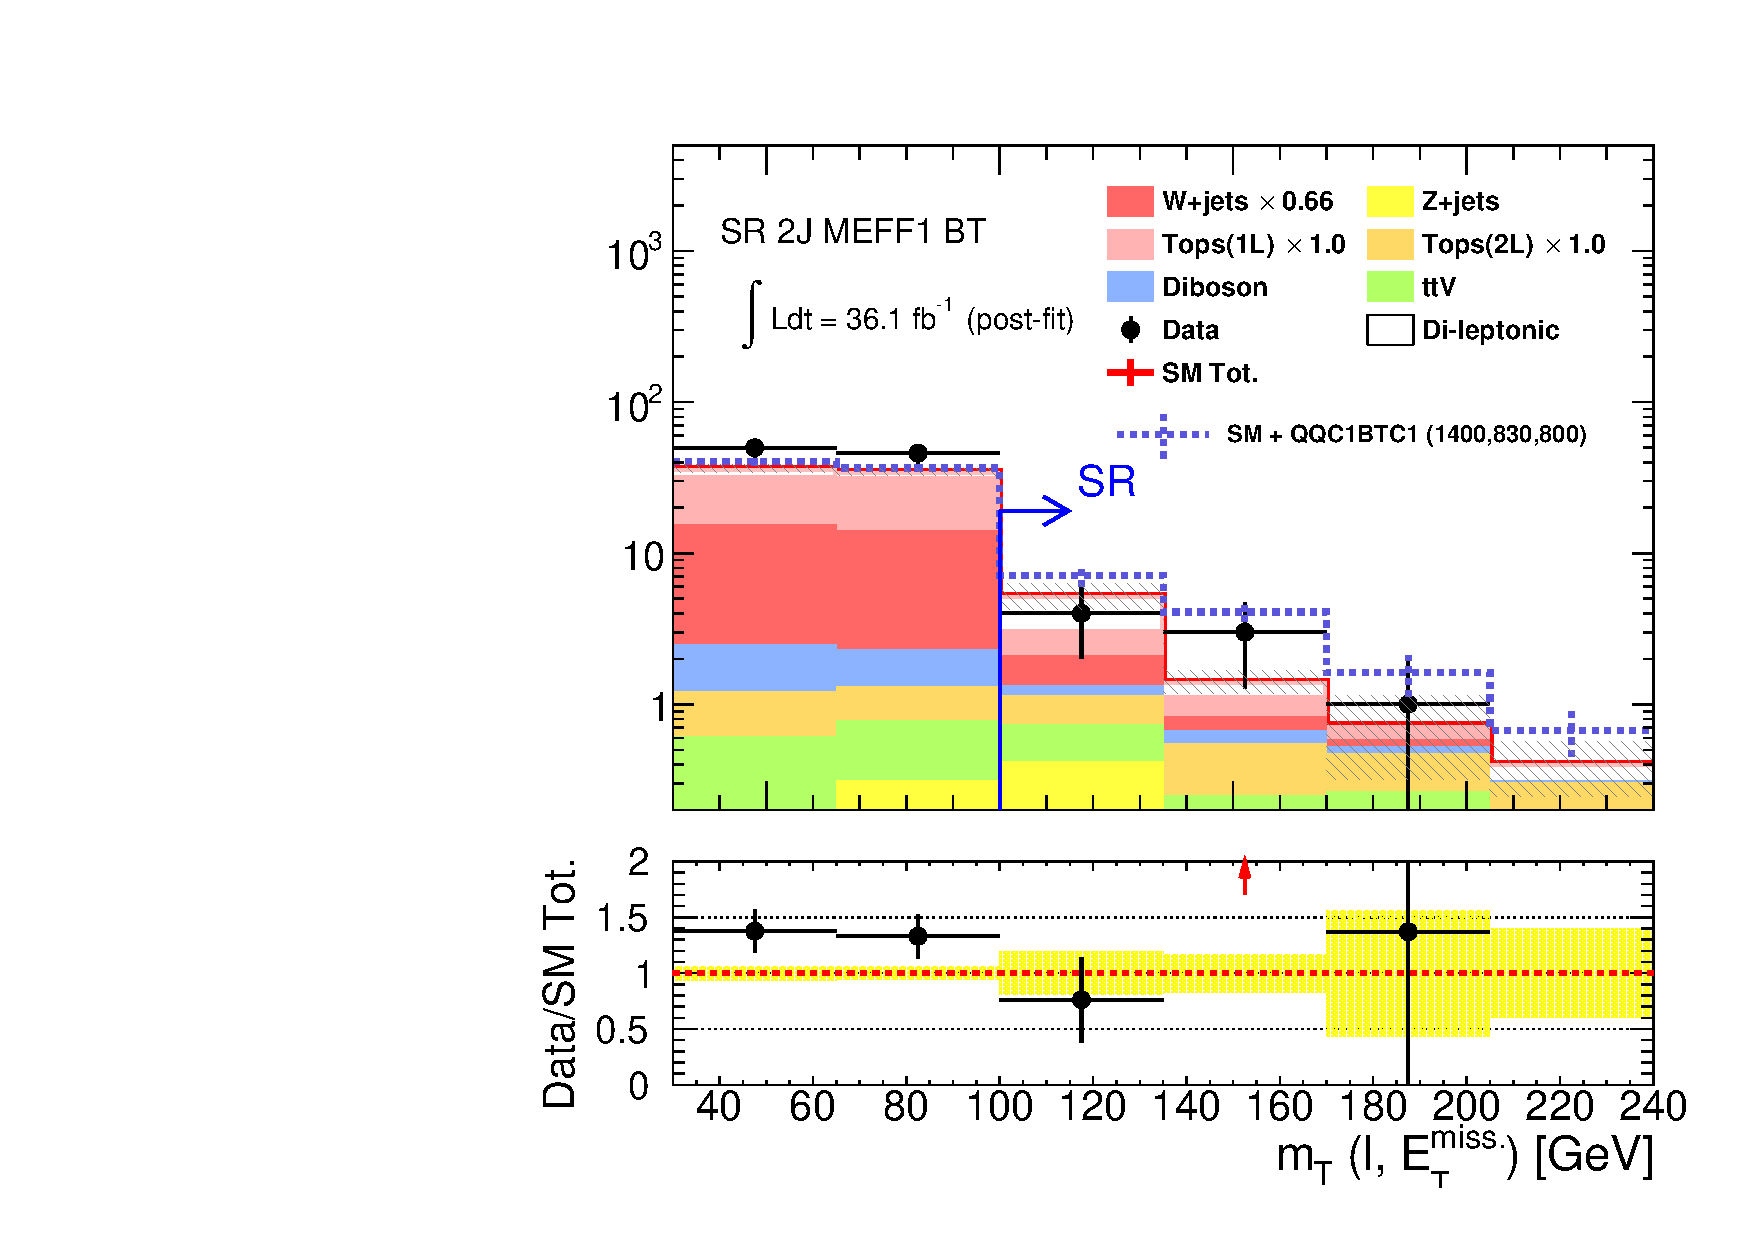
\includegraphics[width=0.41\textwidth]{figures/BGestimation/SRVRpostFit/mt__SR2JMEFF1BT_no_mt_postFit_2SFconfig_noYields_objRep.pdf}}
    \subfigure[]{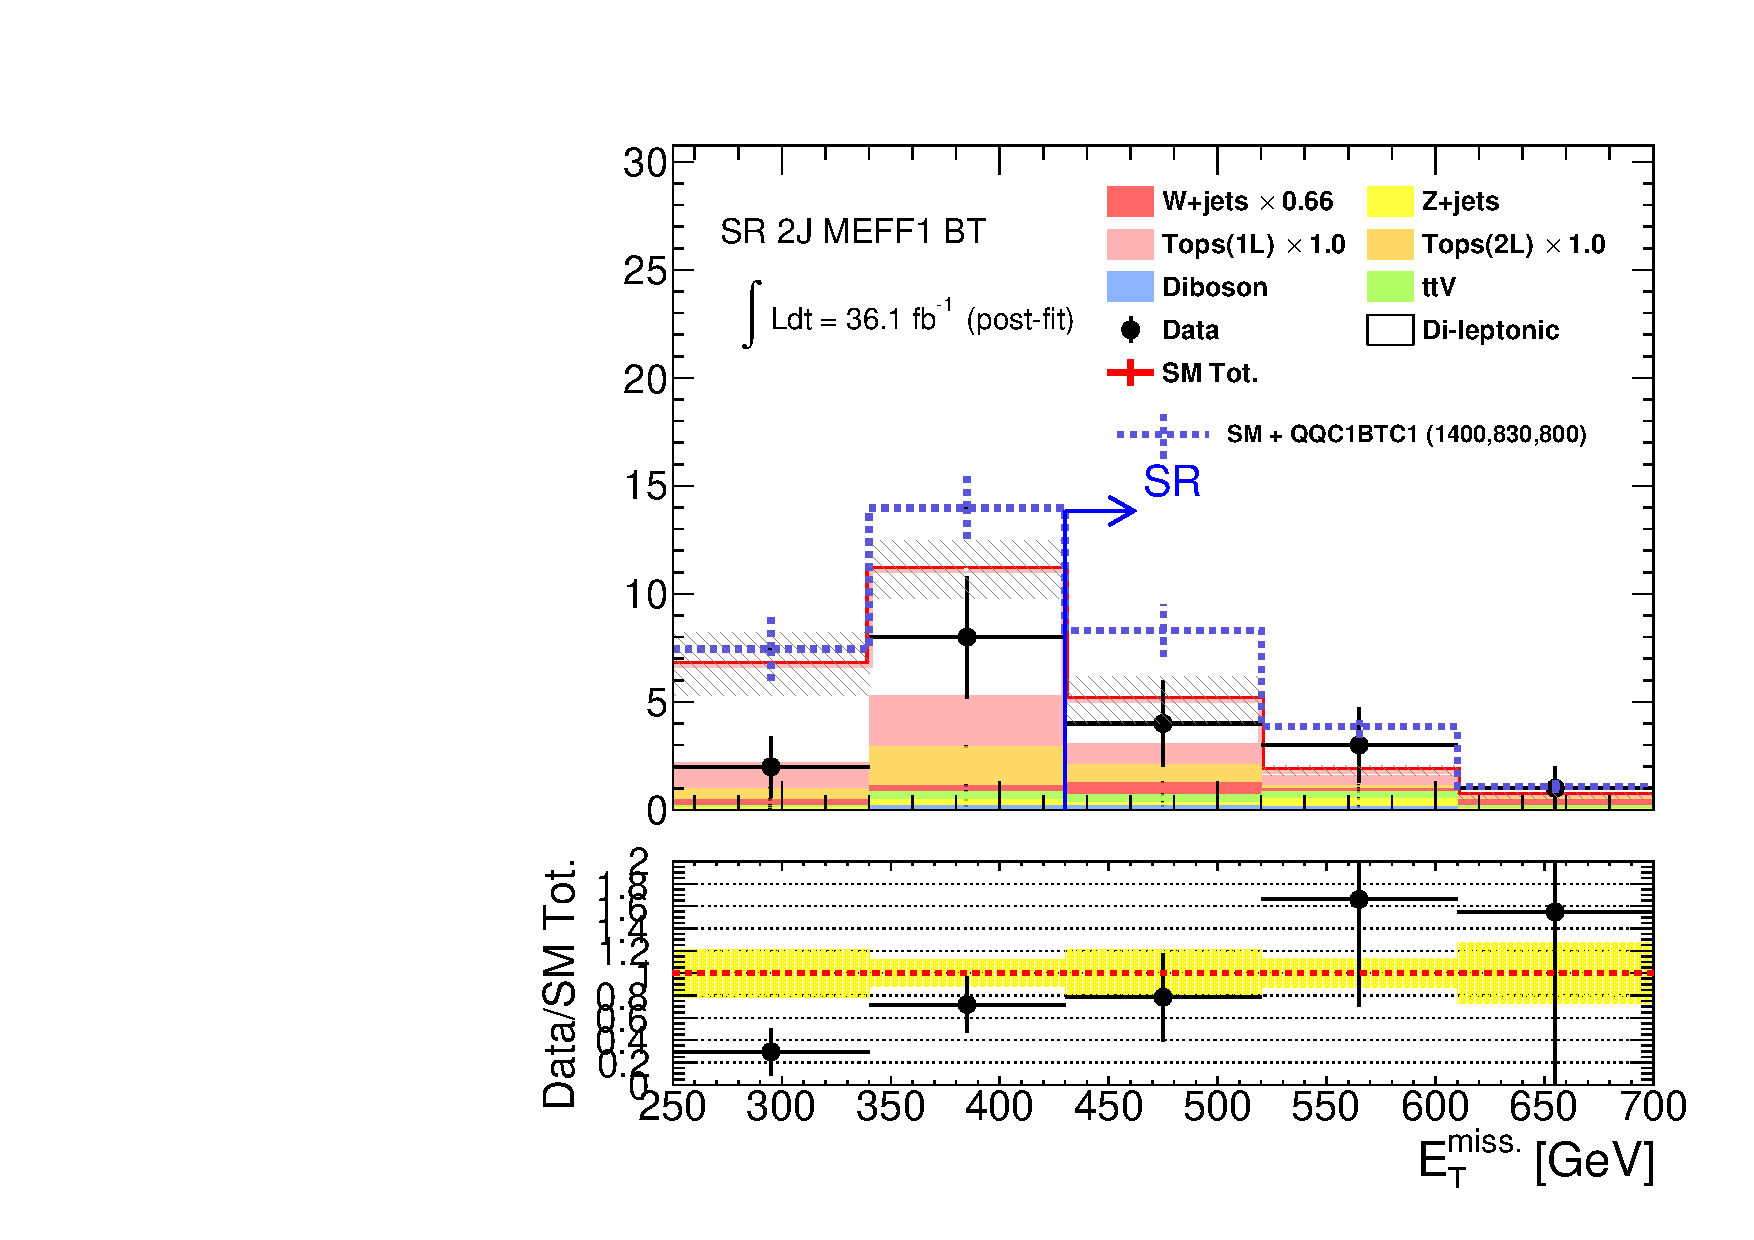
\includegraphics[width=0.41\textwidth]{figures/BGestimation/SRVRpostFit/met__SR2JMEFF1BT_no_met_postFit_2SFconfig_noYields_objRep.pdf}}
    \subfigure[]{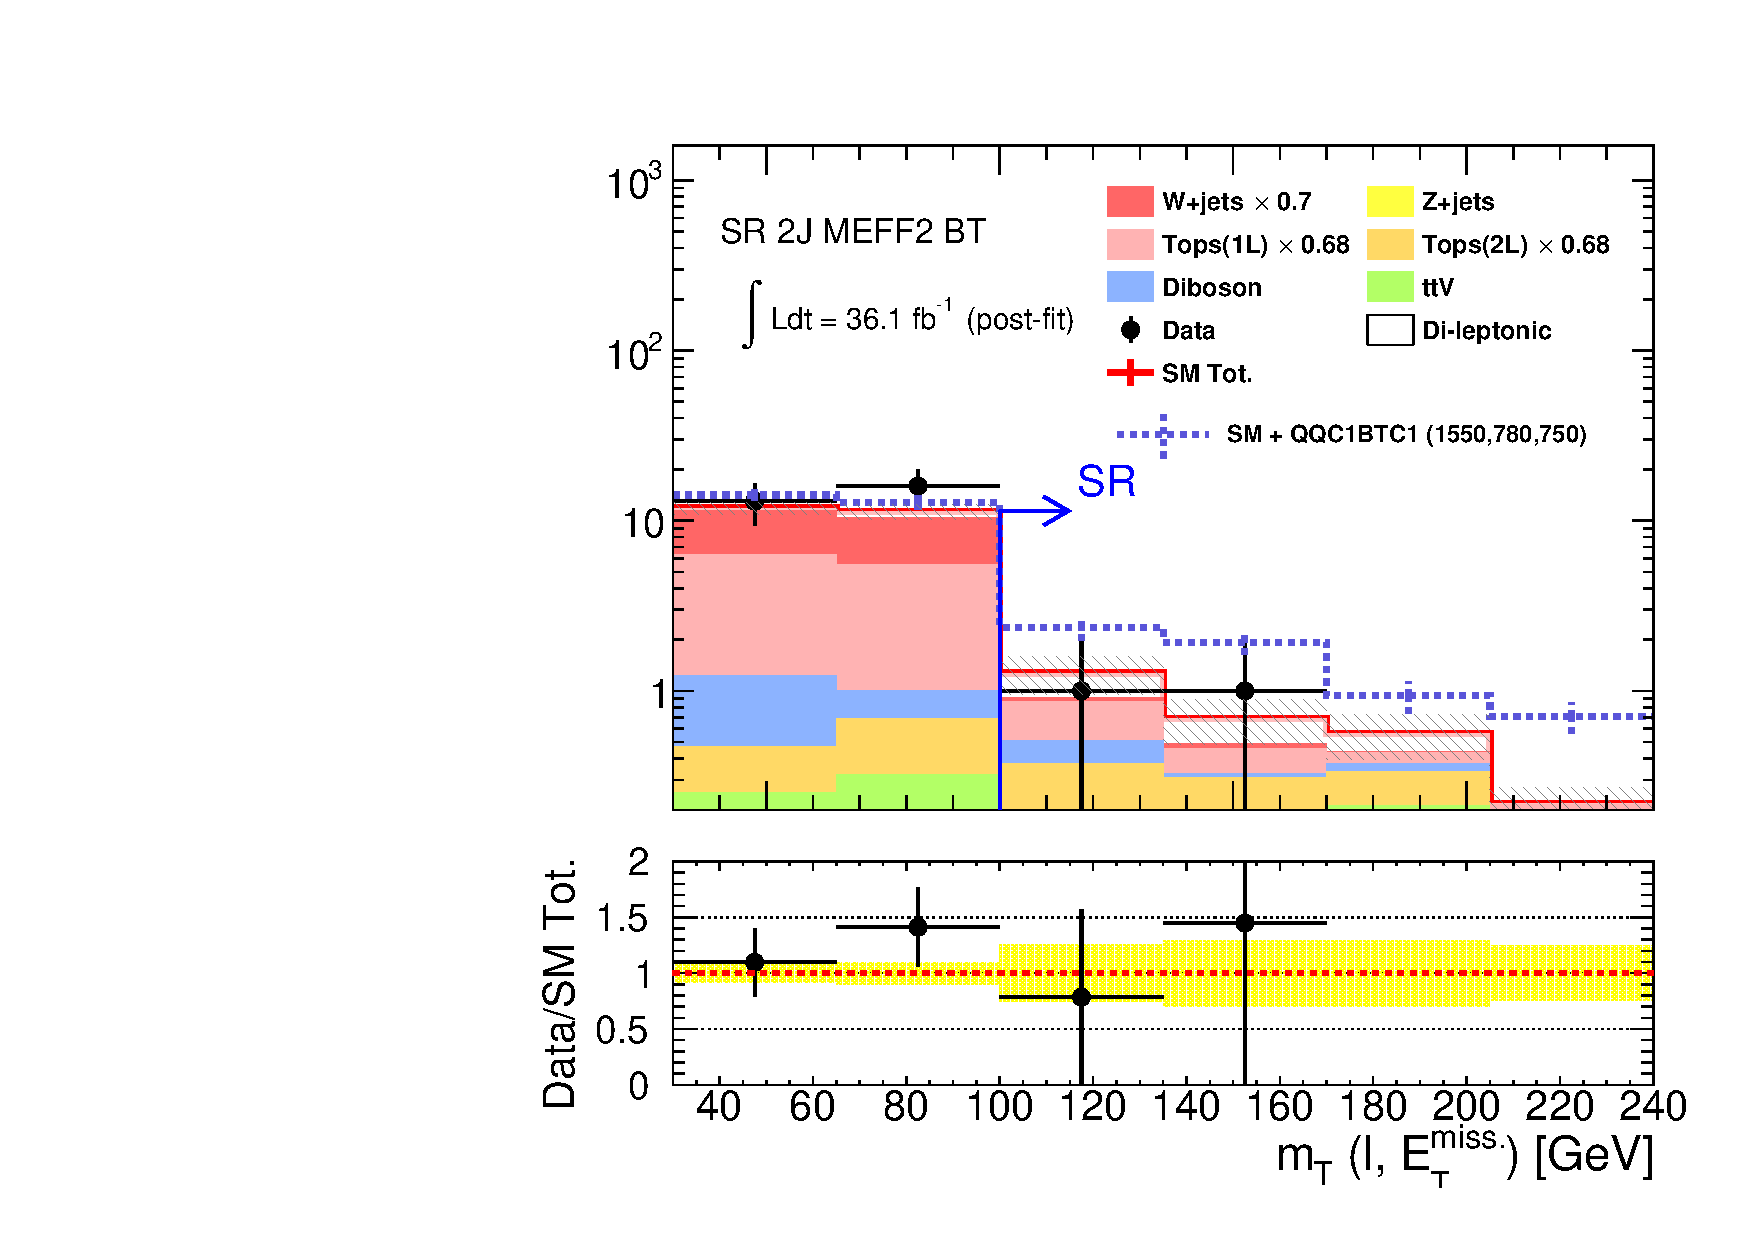
\includegraphics[width=0.41\textwidth]{figures/BGestimation/SRVRpostFit/mt__SR2JMEFF2BT_no_mt_postFit_2SFconfig_noYields_objRep.pdf}}
    \subfigure[]{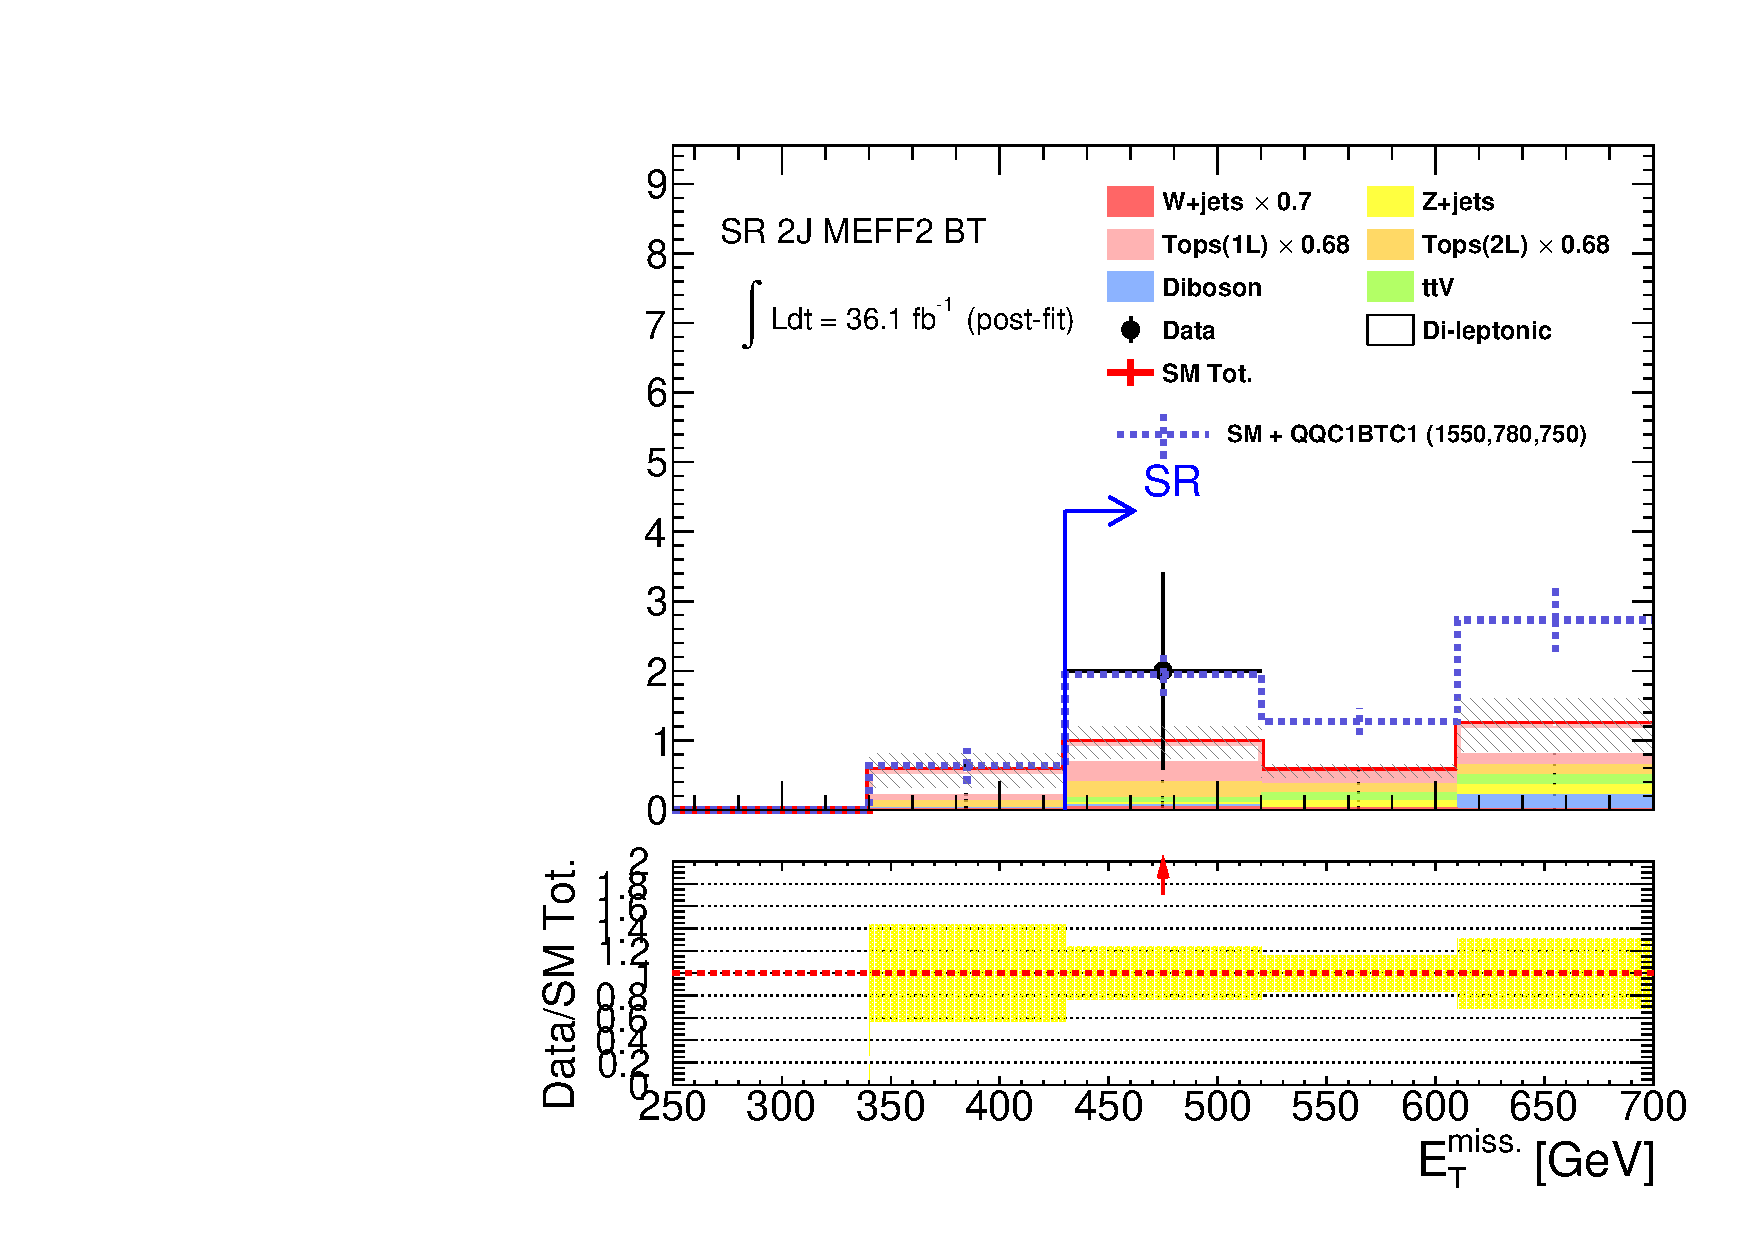
\includegraphics[width=0.41\textwidth]{figures/BGestimation/SRVRpostFit/met__SR2JMEFF2BT_no_met_postFit_2SFconfig_noYields_objRep.pdf}}
    \subfigure[]{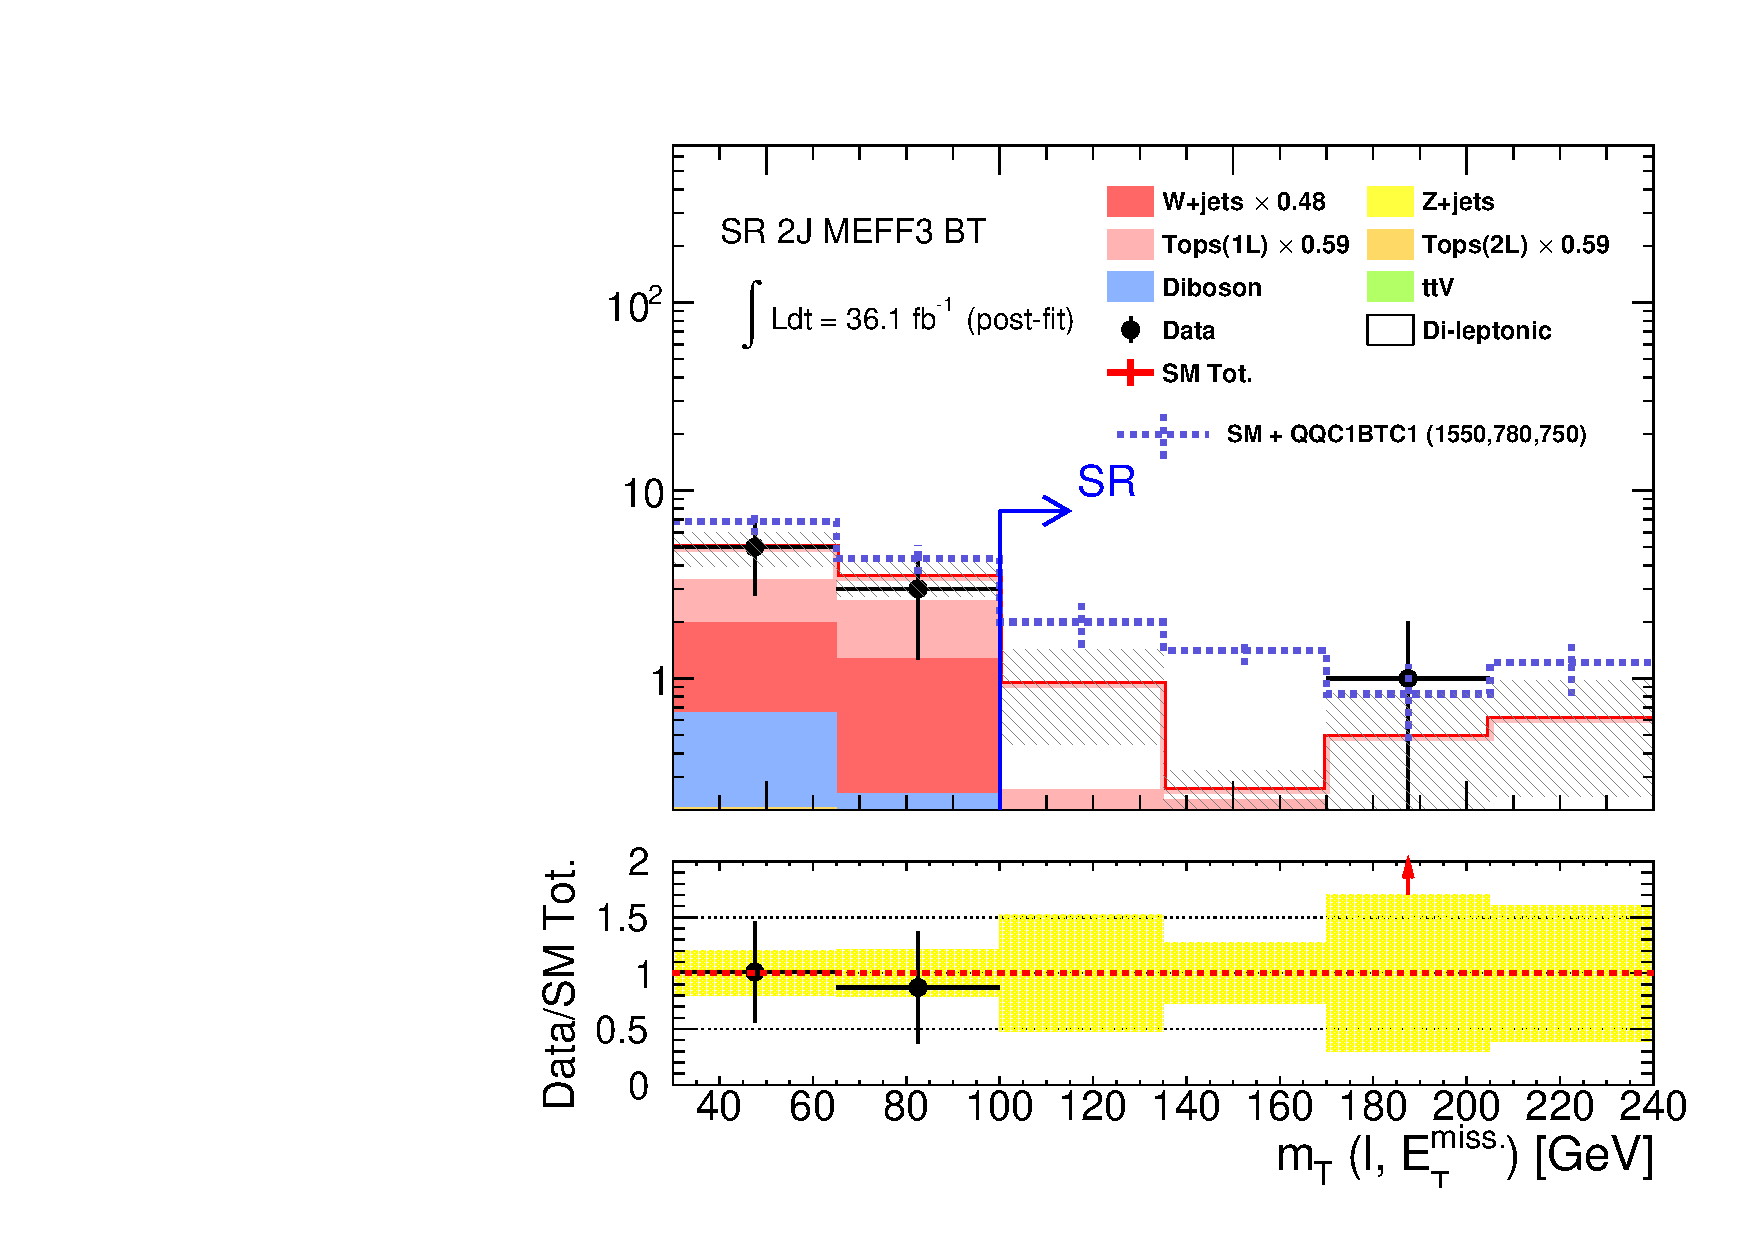
\includegraphics[width=0.41\textwidth]{figures/BGestimation/SRVRpostFit/mt__SR2JMEFF3BT_no_mt_postFit_2SFconfig_noYields_objRep.pdf}}
    \subfigure[]{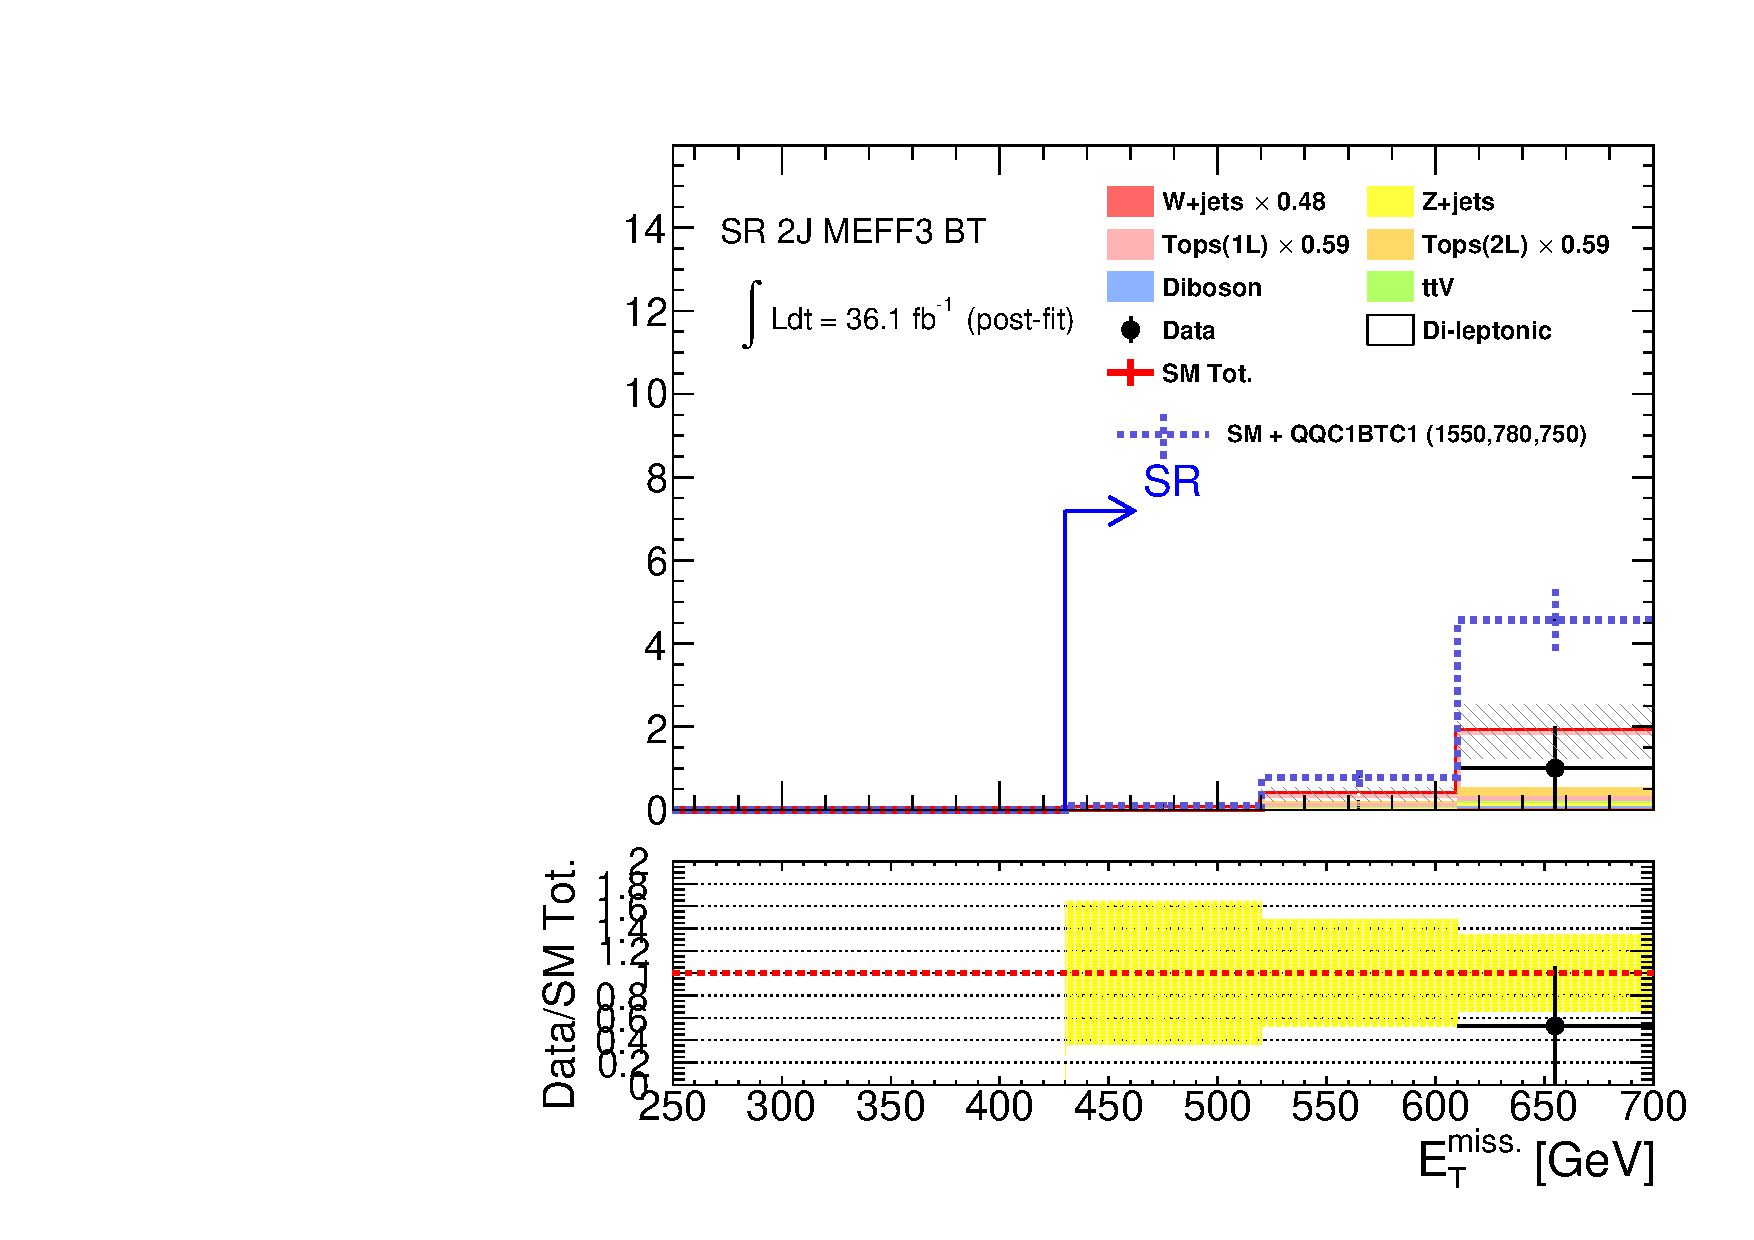
\includegraphics[width=0.41\textwidth]{figures/BGestimation/SRVRpostFit/met__SR2JMEFF3BT_no_met_postFit_2SFconfig_noYields_objRep.pdf}}
   \caption{
     Post-fit distruibution of (left) $\mt$, and (right) $\met$.
     (a,b) SR 2J-$\meffIncFirst$ BT.
     (c,d) SR 2J-$\meffIncSecond$ BT.
     (e,f) SR 2J-$\meffIncThird$ BT. 
     The yellow band in the bottom panel represents statistical error. The overflow is included in the highest bin.  
     \label{fig::BGestimation::SRVRpostFit::SR2JBT}
   }
\end{figure}


\clearpage
\begin{figure}[h]
  \centering
    \subfigure[]{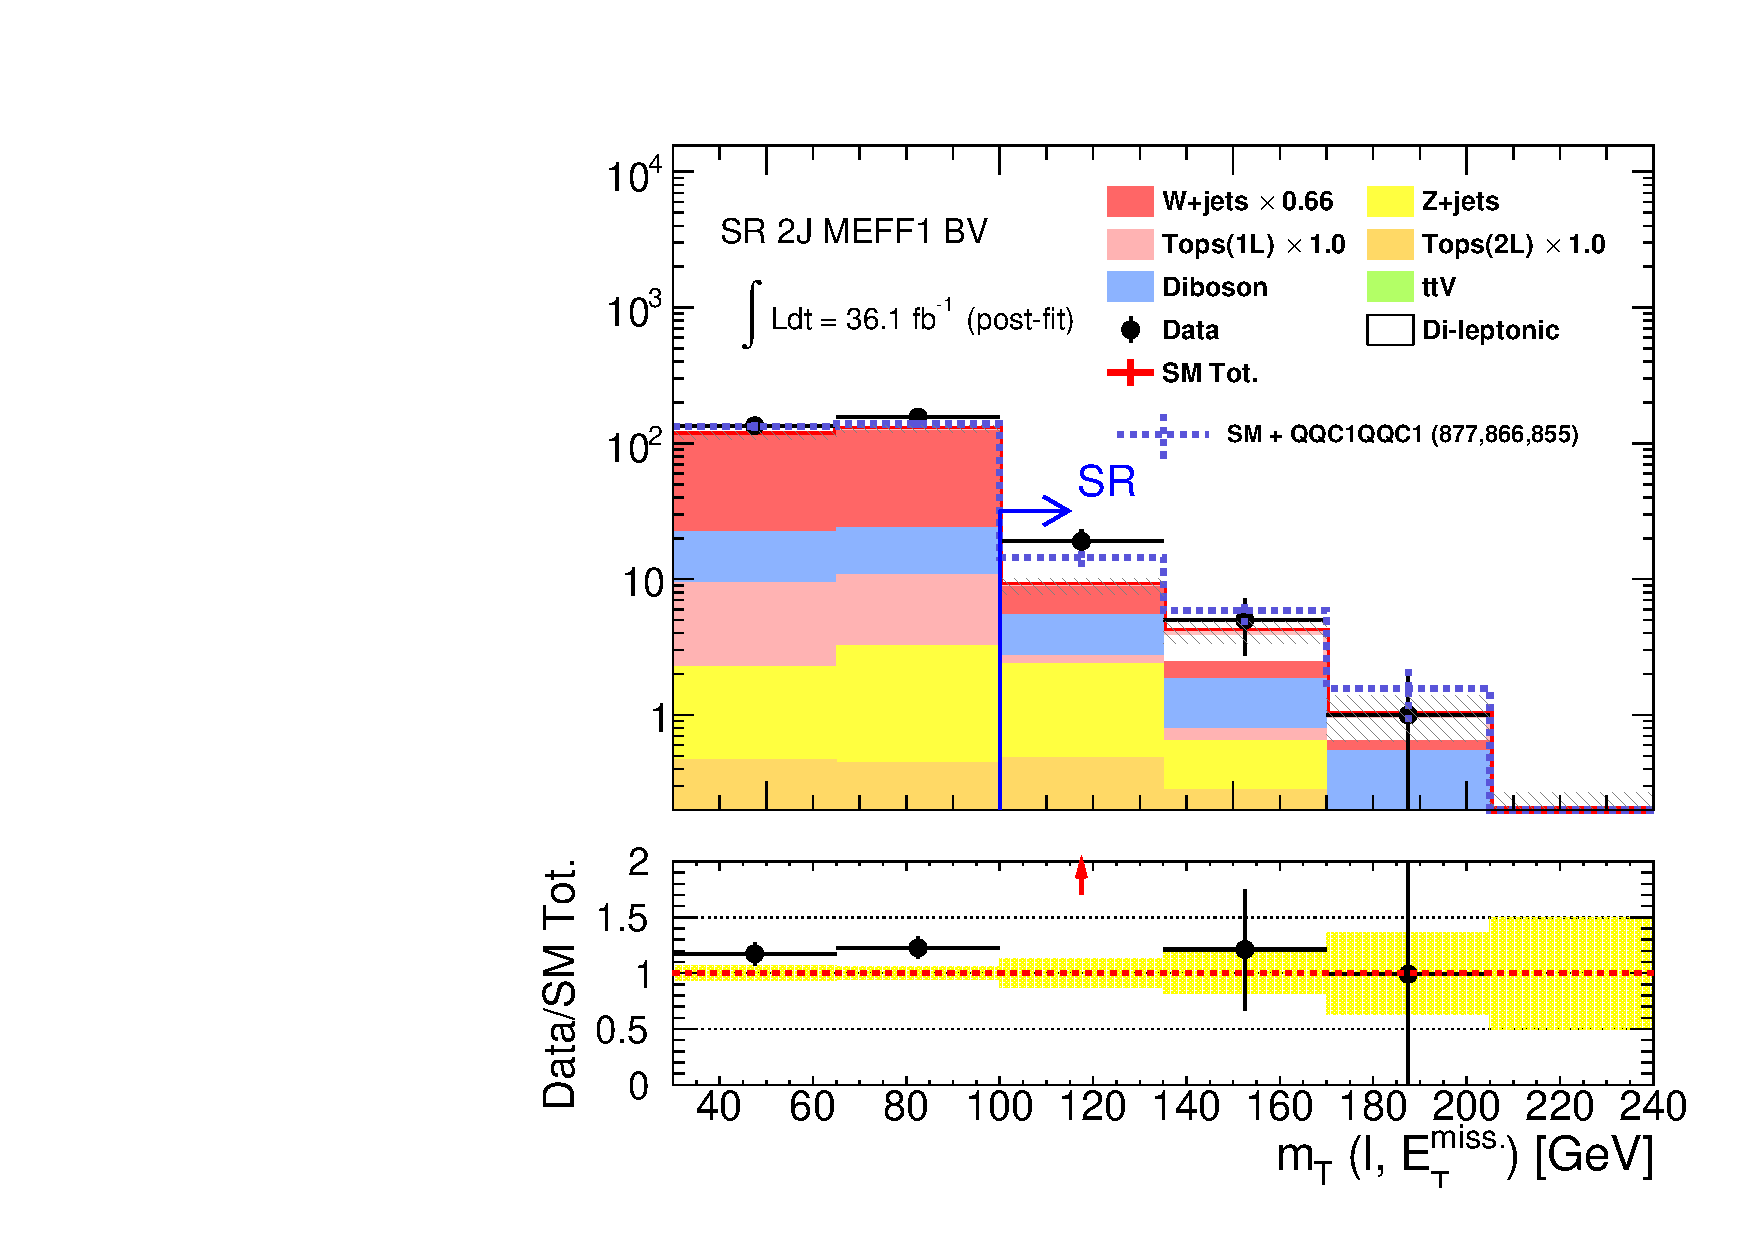
\includegraphics[width=0.41\textwidth]{figures/BGestimation/SRVRpostFit/mt__SR2JMEFF1BV_no_mt_postFit_2SFconfig_noYields_objRep.pdf}}
    \subfigure[]{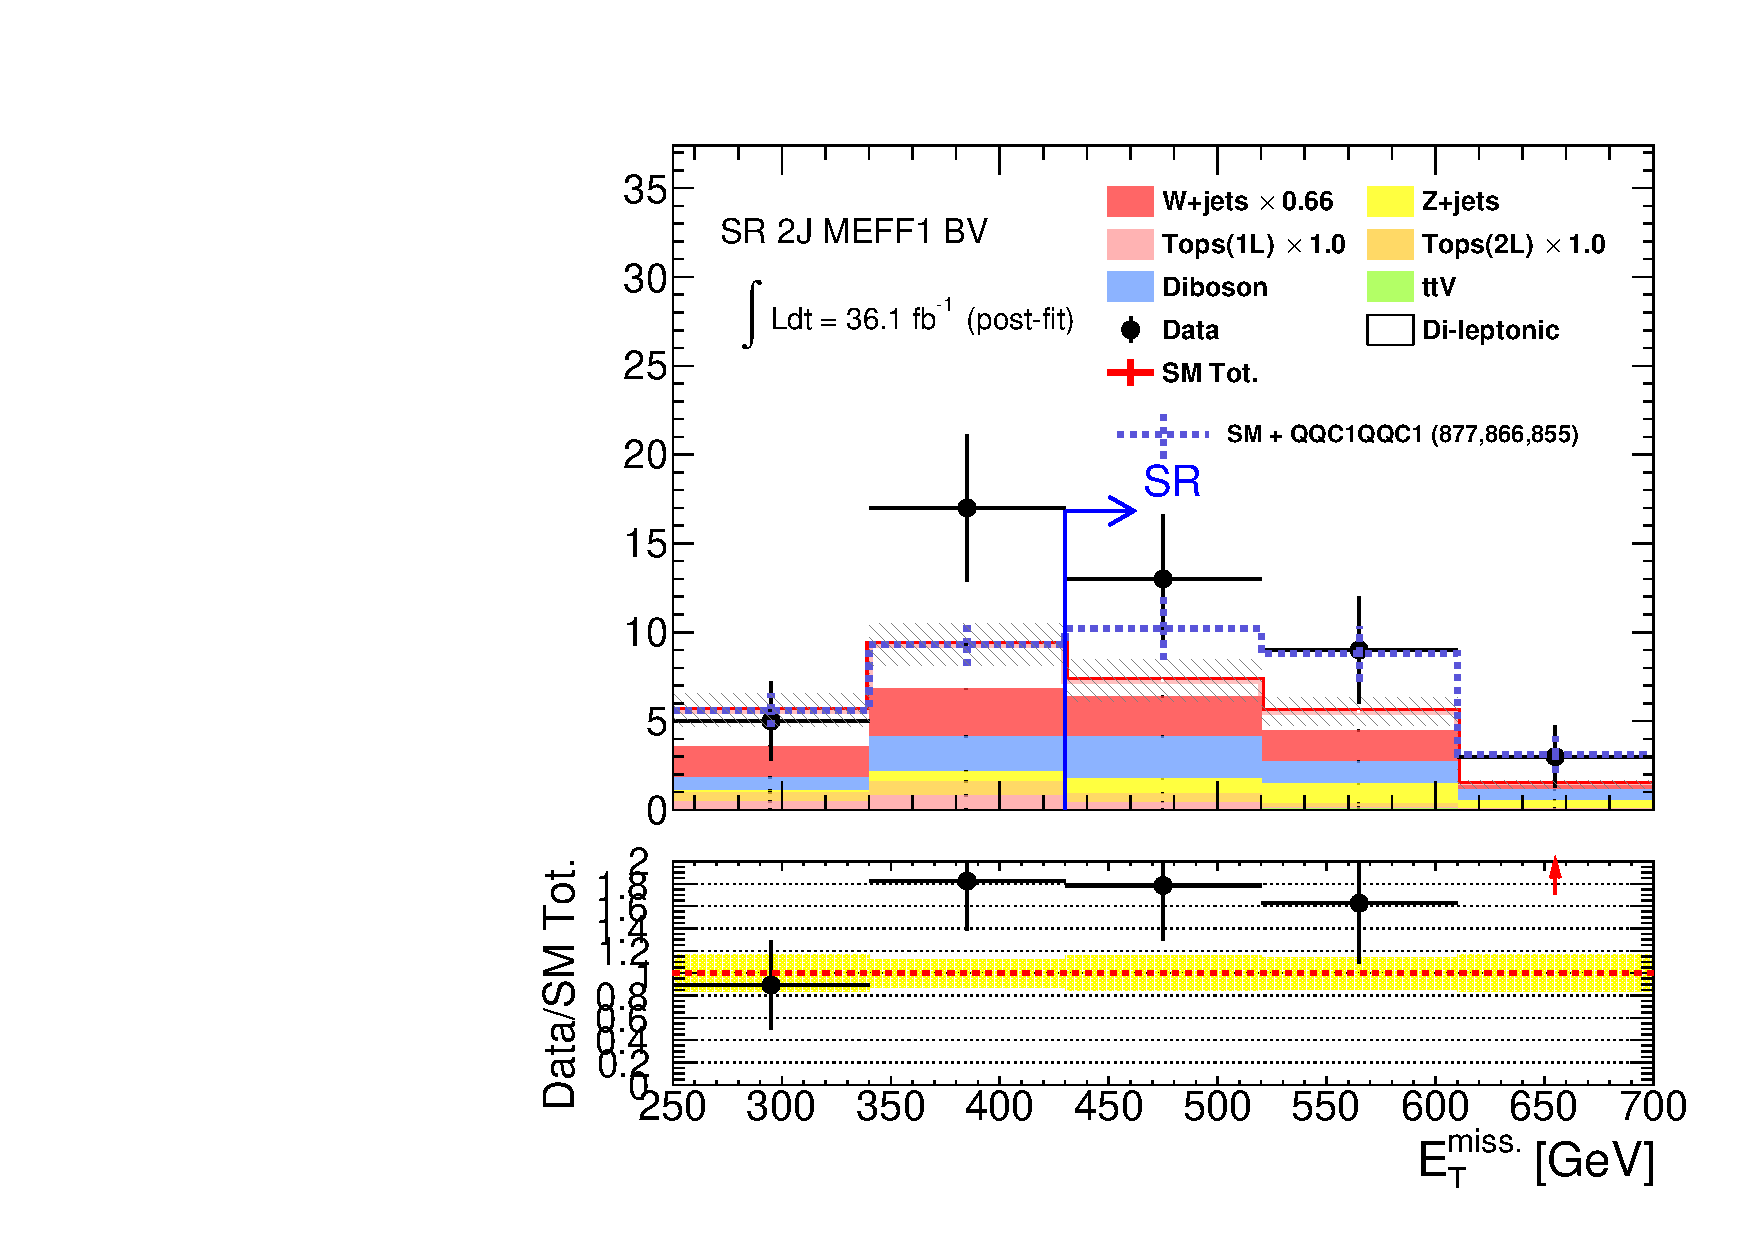
\includegraphics[width=0.41\textwidth]{figures/BGestimation/SRVRpostFit/met__SR2JMEFF1BV_no_met_postFit_2SFconfig_noYields_objRep.pdf}}
    \subfigure[]{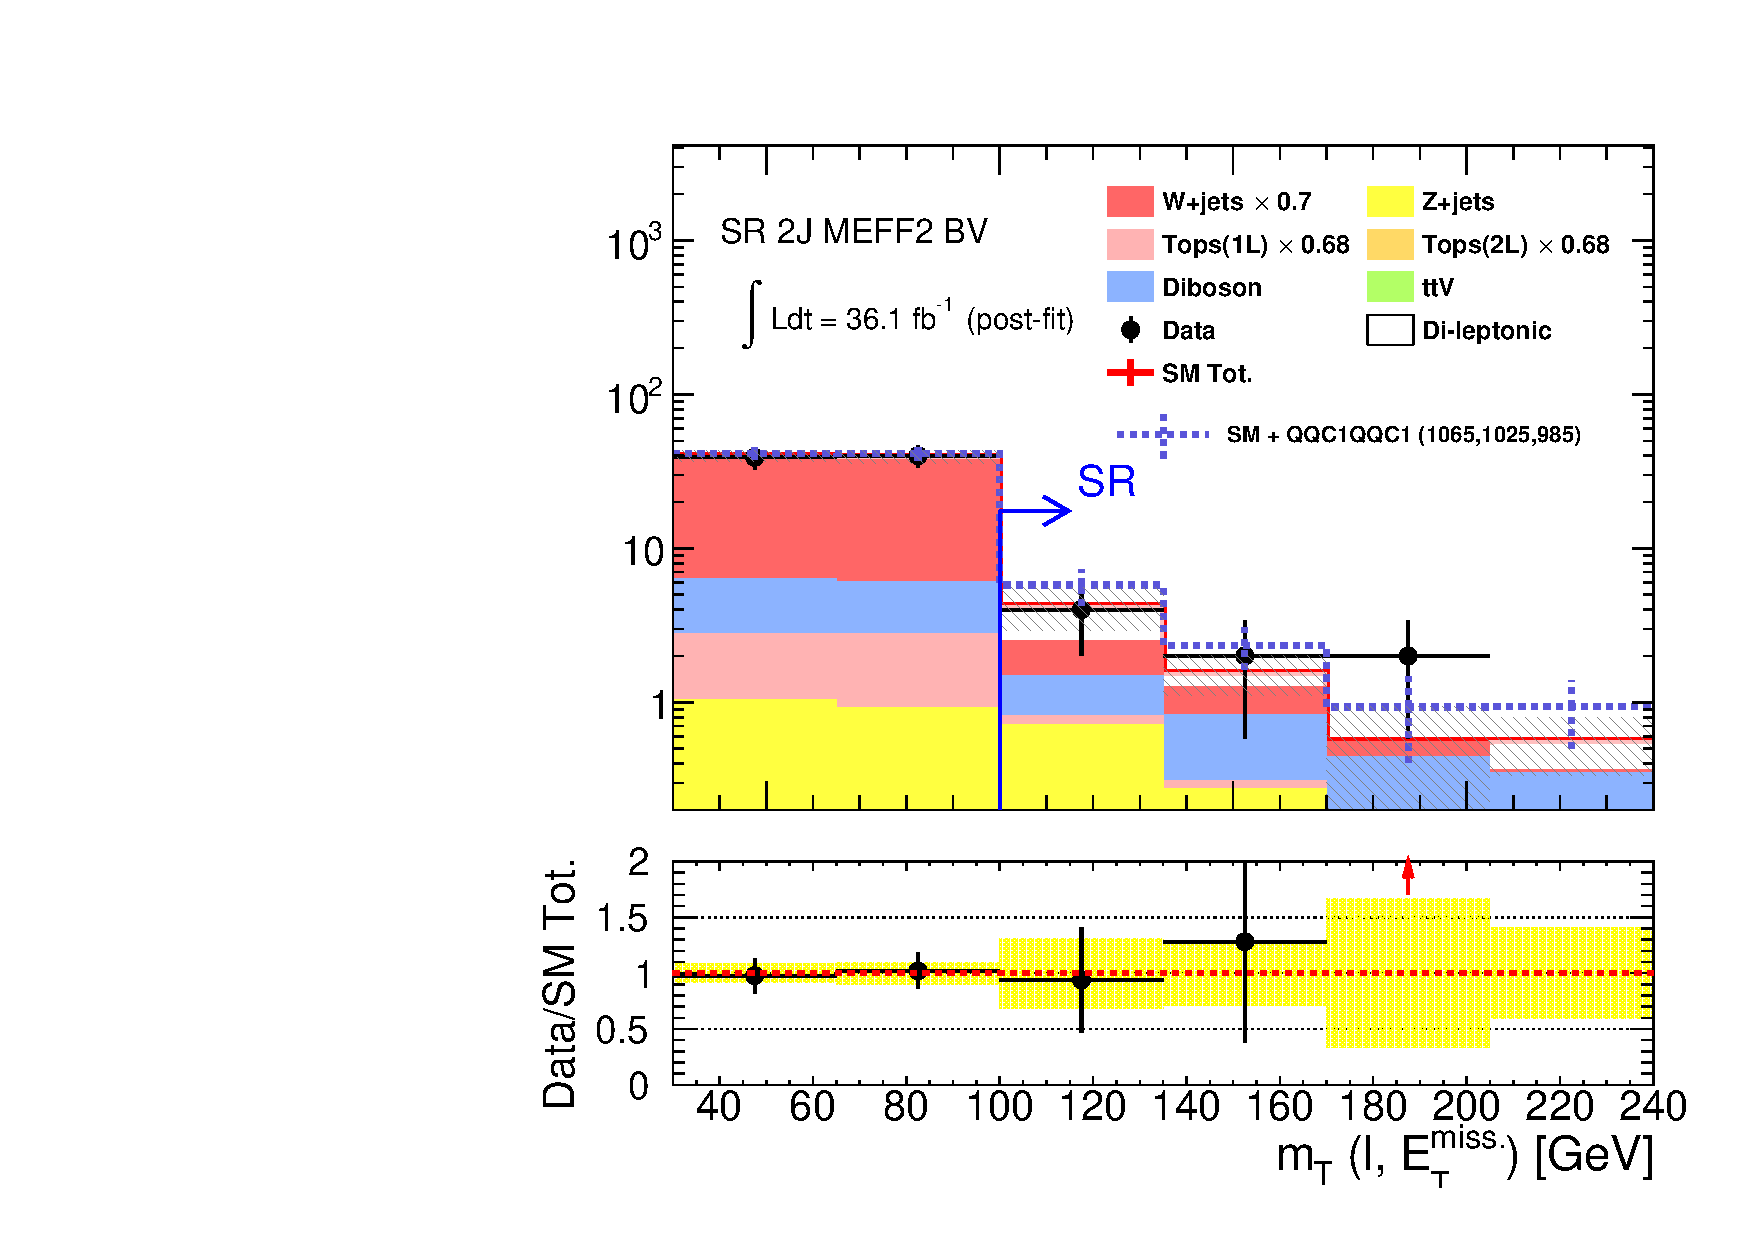
\includegraphics[width=0.41\textwidth]{figures/BGestimation/SRVRpostFit/mt__SR2JMEFF2BV_no_mt_postFit_2SFconfig_noYields_objRep.pdf}}
    \subfigure[]{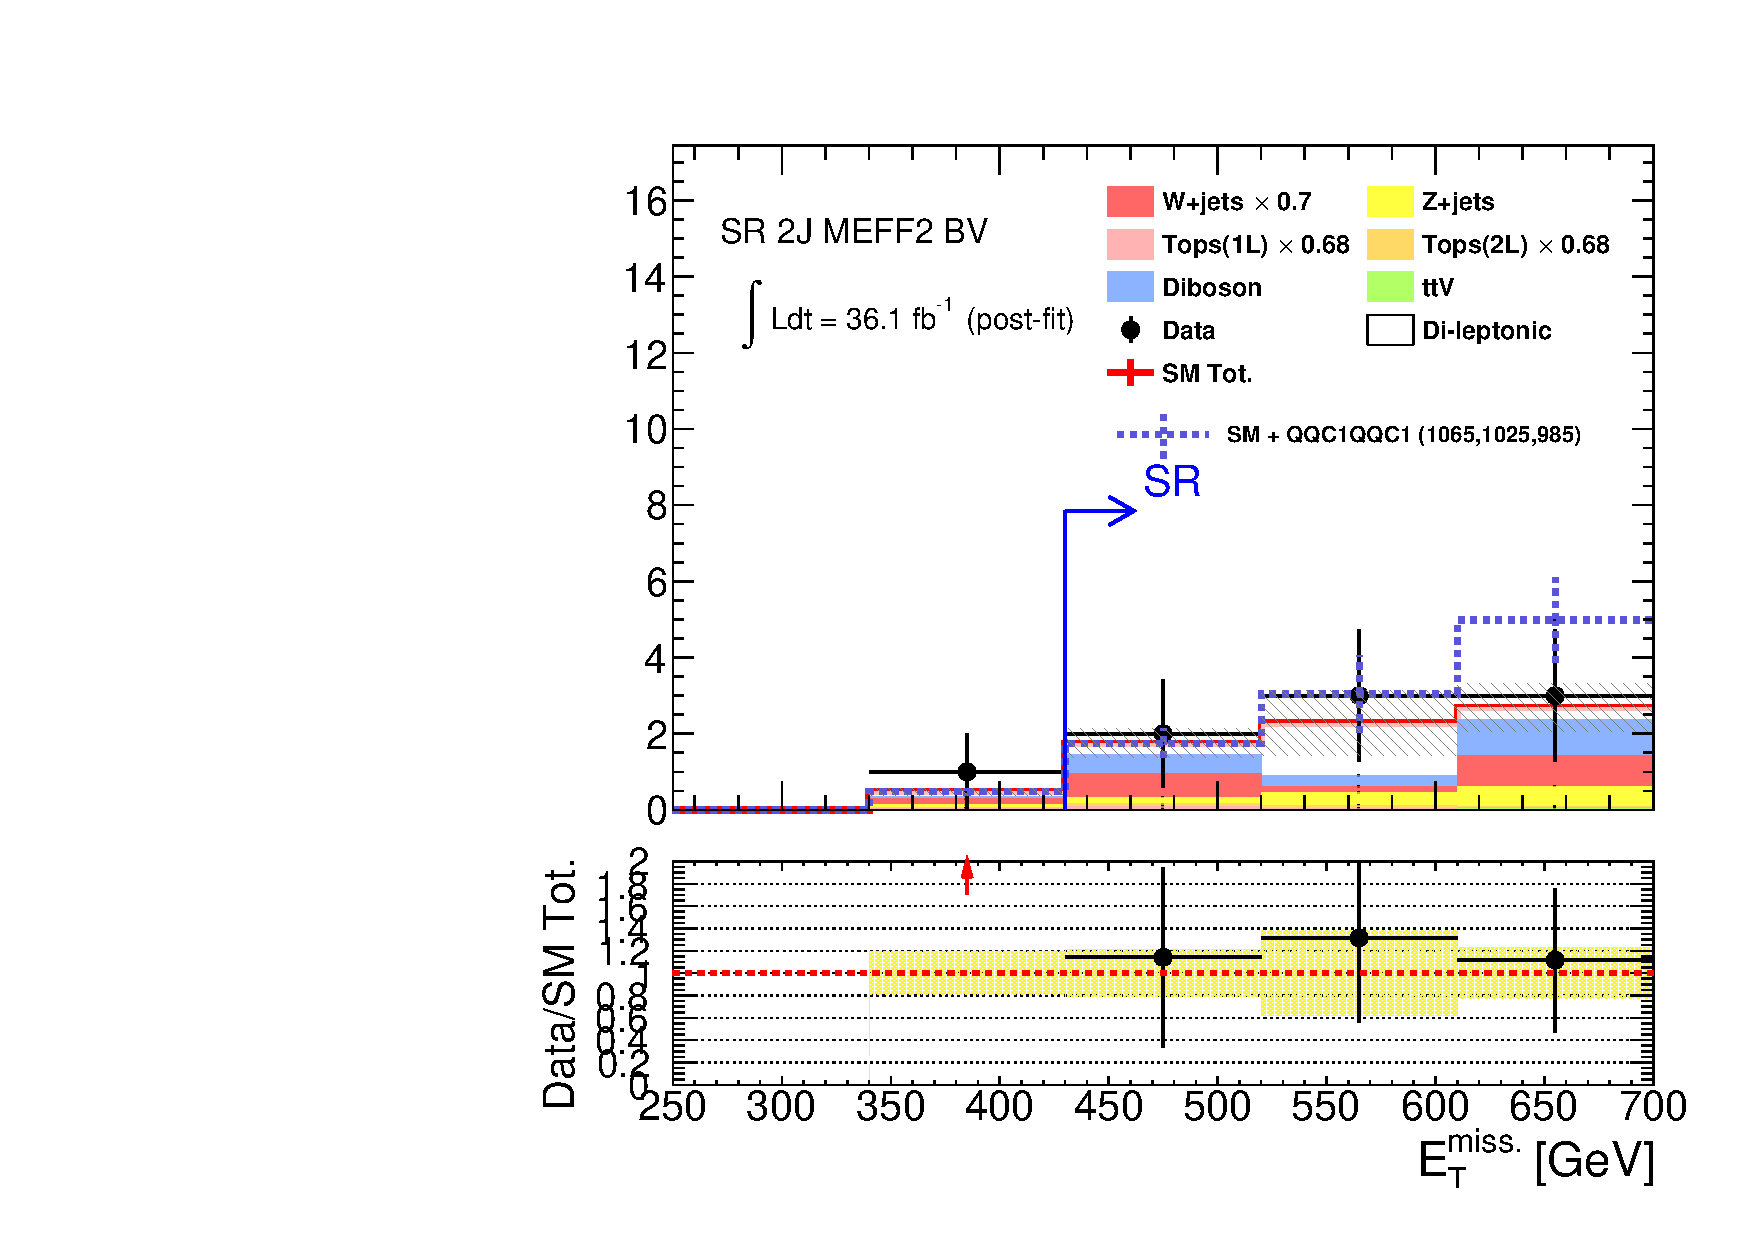
\includegraphics[width=0.41\textwidth]{figures/BGestimation/SRVRpostFit/met__SR2JMEFF2BV_no_met_postFit_2SFconfig_noYields_objRep.pdf}}
    \subfigure[]{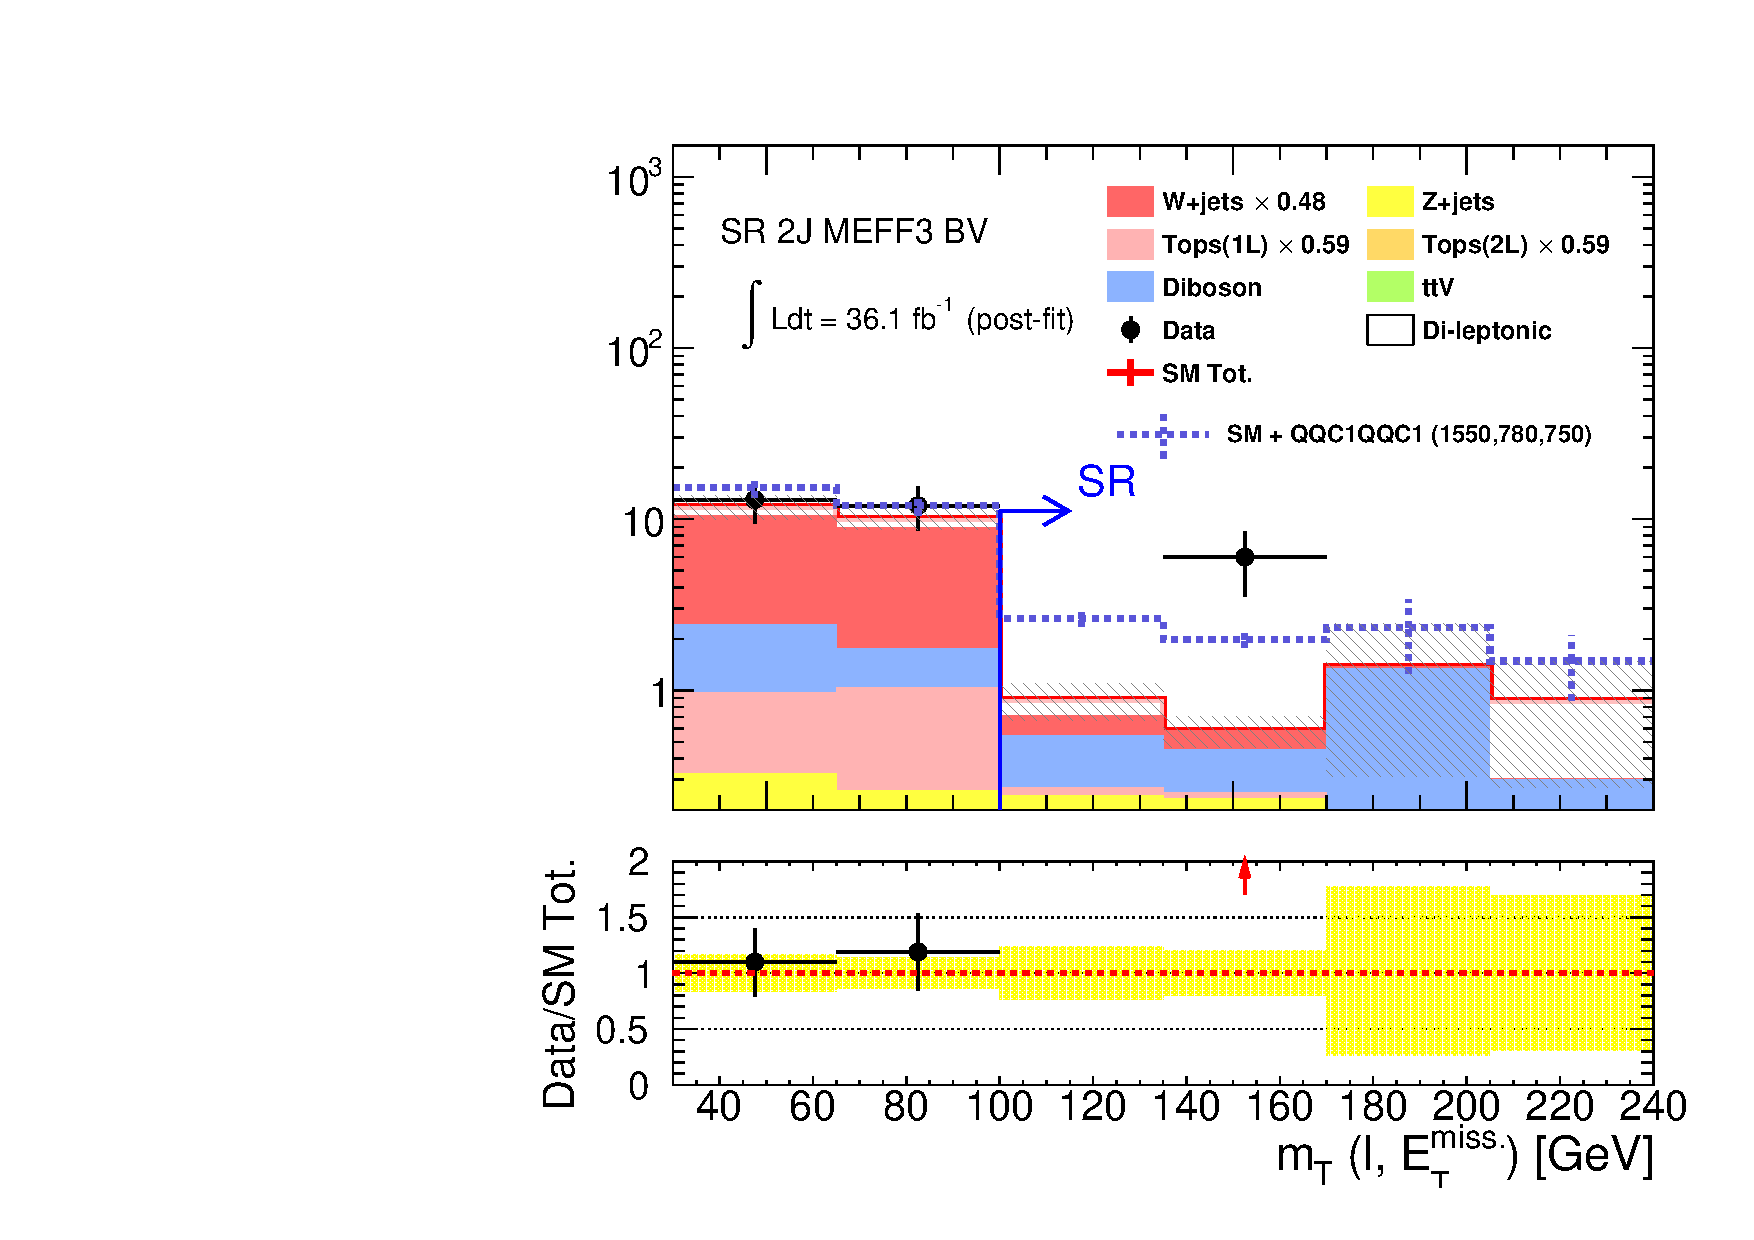
\includegraphics[width=0.41\textwidth]{figures/BGestimation/SRVRpostFit/mt__SR2JMEFF3BV_no_mt_postFit_2SFconfig_noYields_objRep.pdf}}
    \subfigure[]{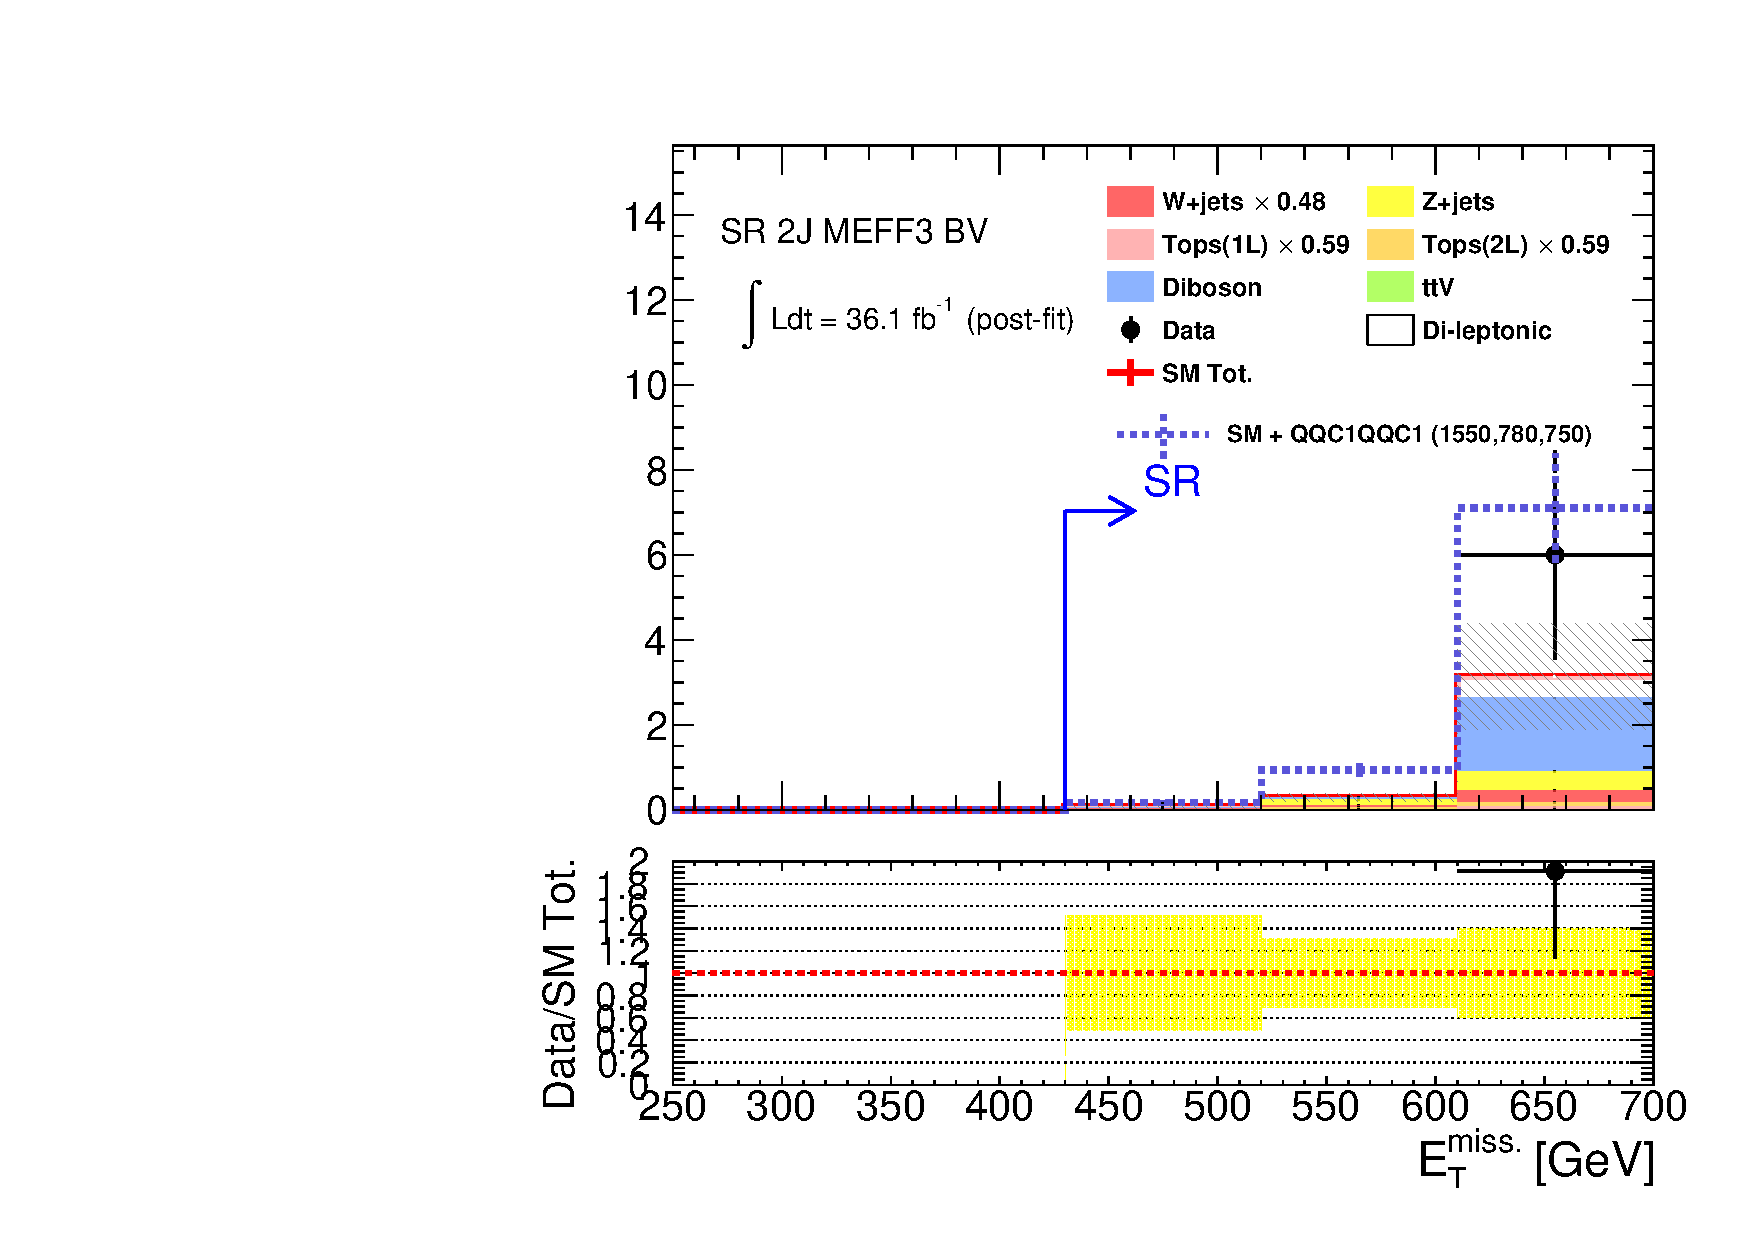
\includegraphics[width=0.41\textwidth]{figures/BGestimation/SRVRpostFit/met__SR2JMEFF3BV_no_met_postFit_2SFconfig_noYields_objRep.pdf}}
   \caption{
     Post-fit distruibution of (left) $\mt$, and (right) $\met$.
     (a,b) SR 2J-$\meffIncFirst$ BV.
     (c,d) SR 2J-$\meffIncSecond$ BV.
     (e,f) SR 2J-$\meffIncThird$ BV. 
     The yellow band in the bottom panel represents statistical error. The overflow is included in the highest bin.  
     \label{fig::BGestimation::SRVRpostFit::SR2JBV}
   }
\end{figure}
% -------------------------------------



\clearpage
% -------------- 6J ---------
\begin{figure}[h]
  \centering
    \subfigure[]{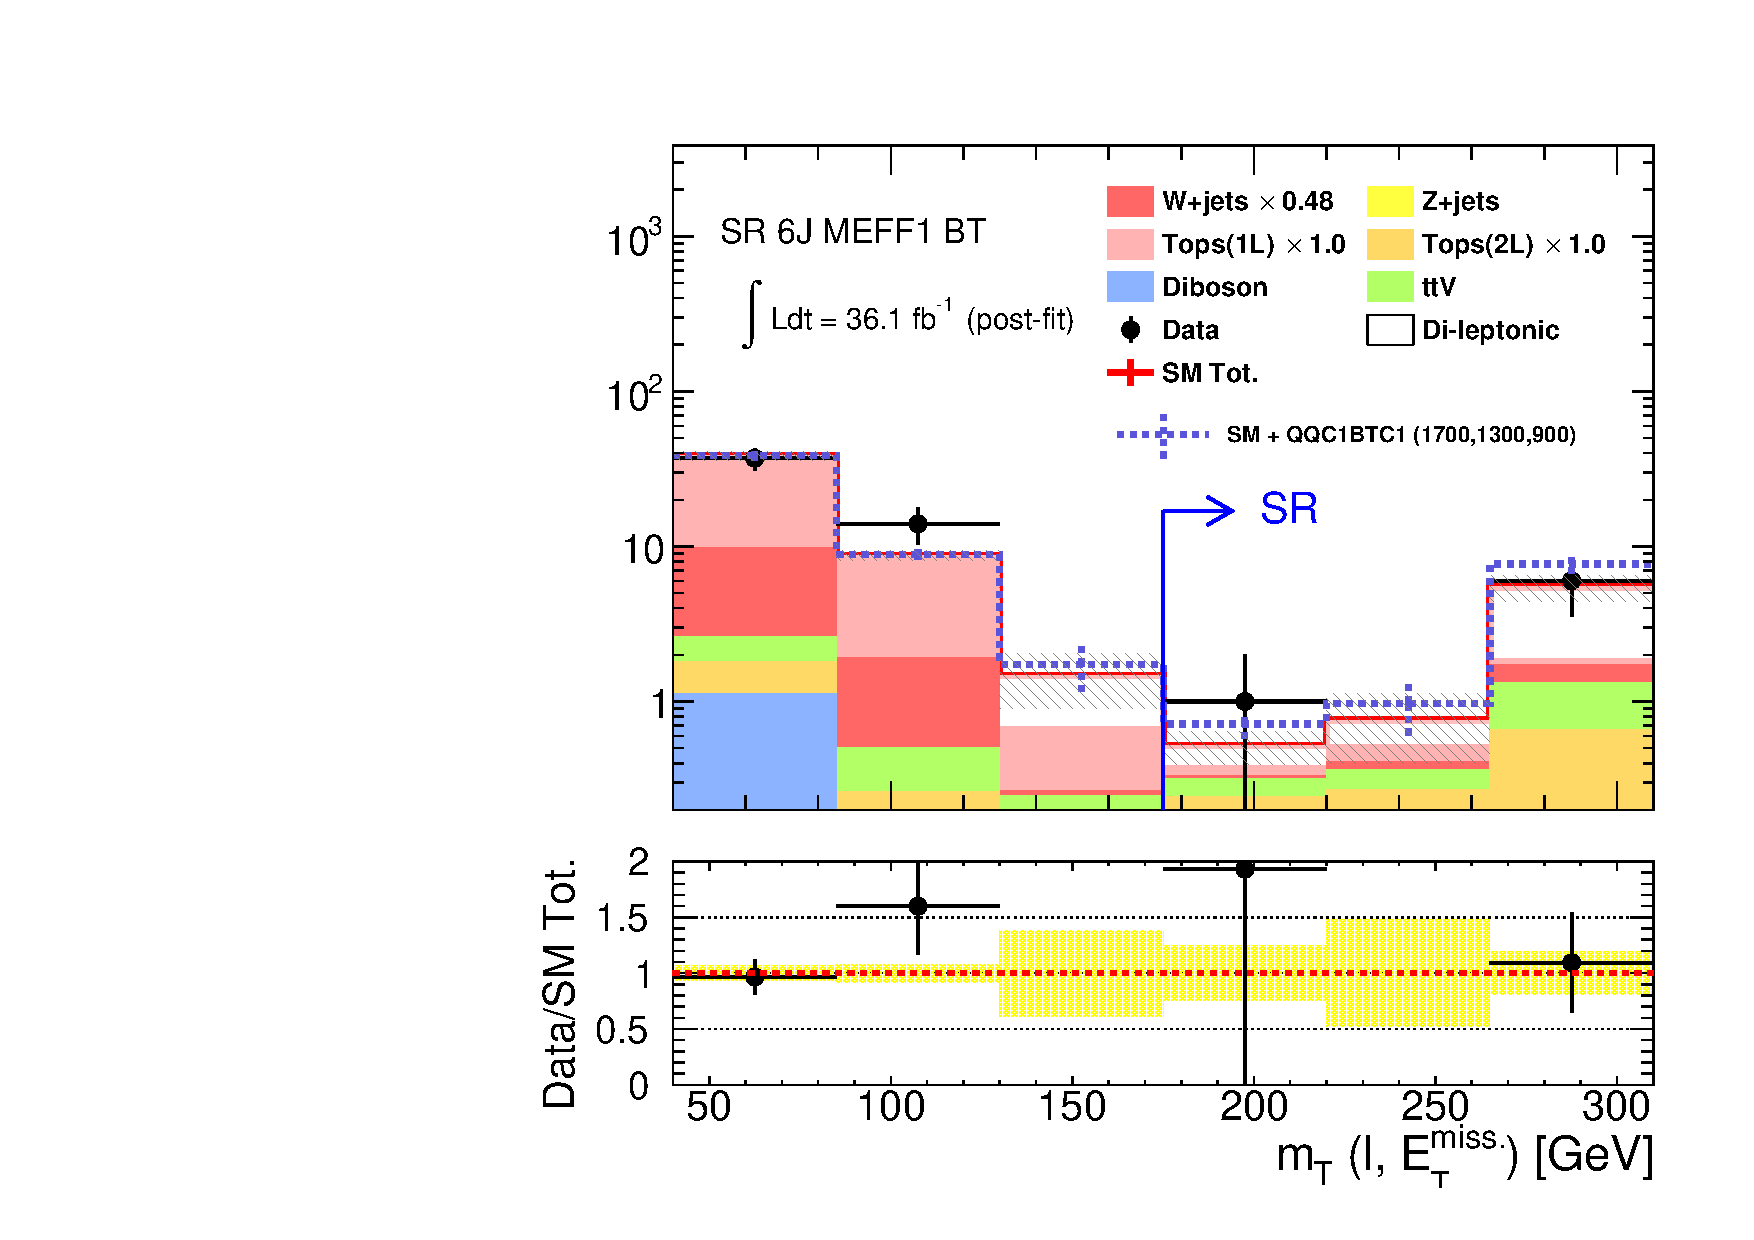
\includegraphics[width=0.41\textwidth]{figures/BGestimation/SRVRpostFit/mt__SR6JMEFF1BT_no_mt_postFit_2SFconfig_noYields_objRep.pdf}}
    \subfigure[]{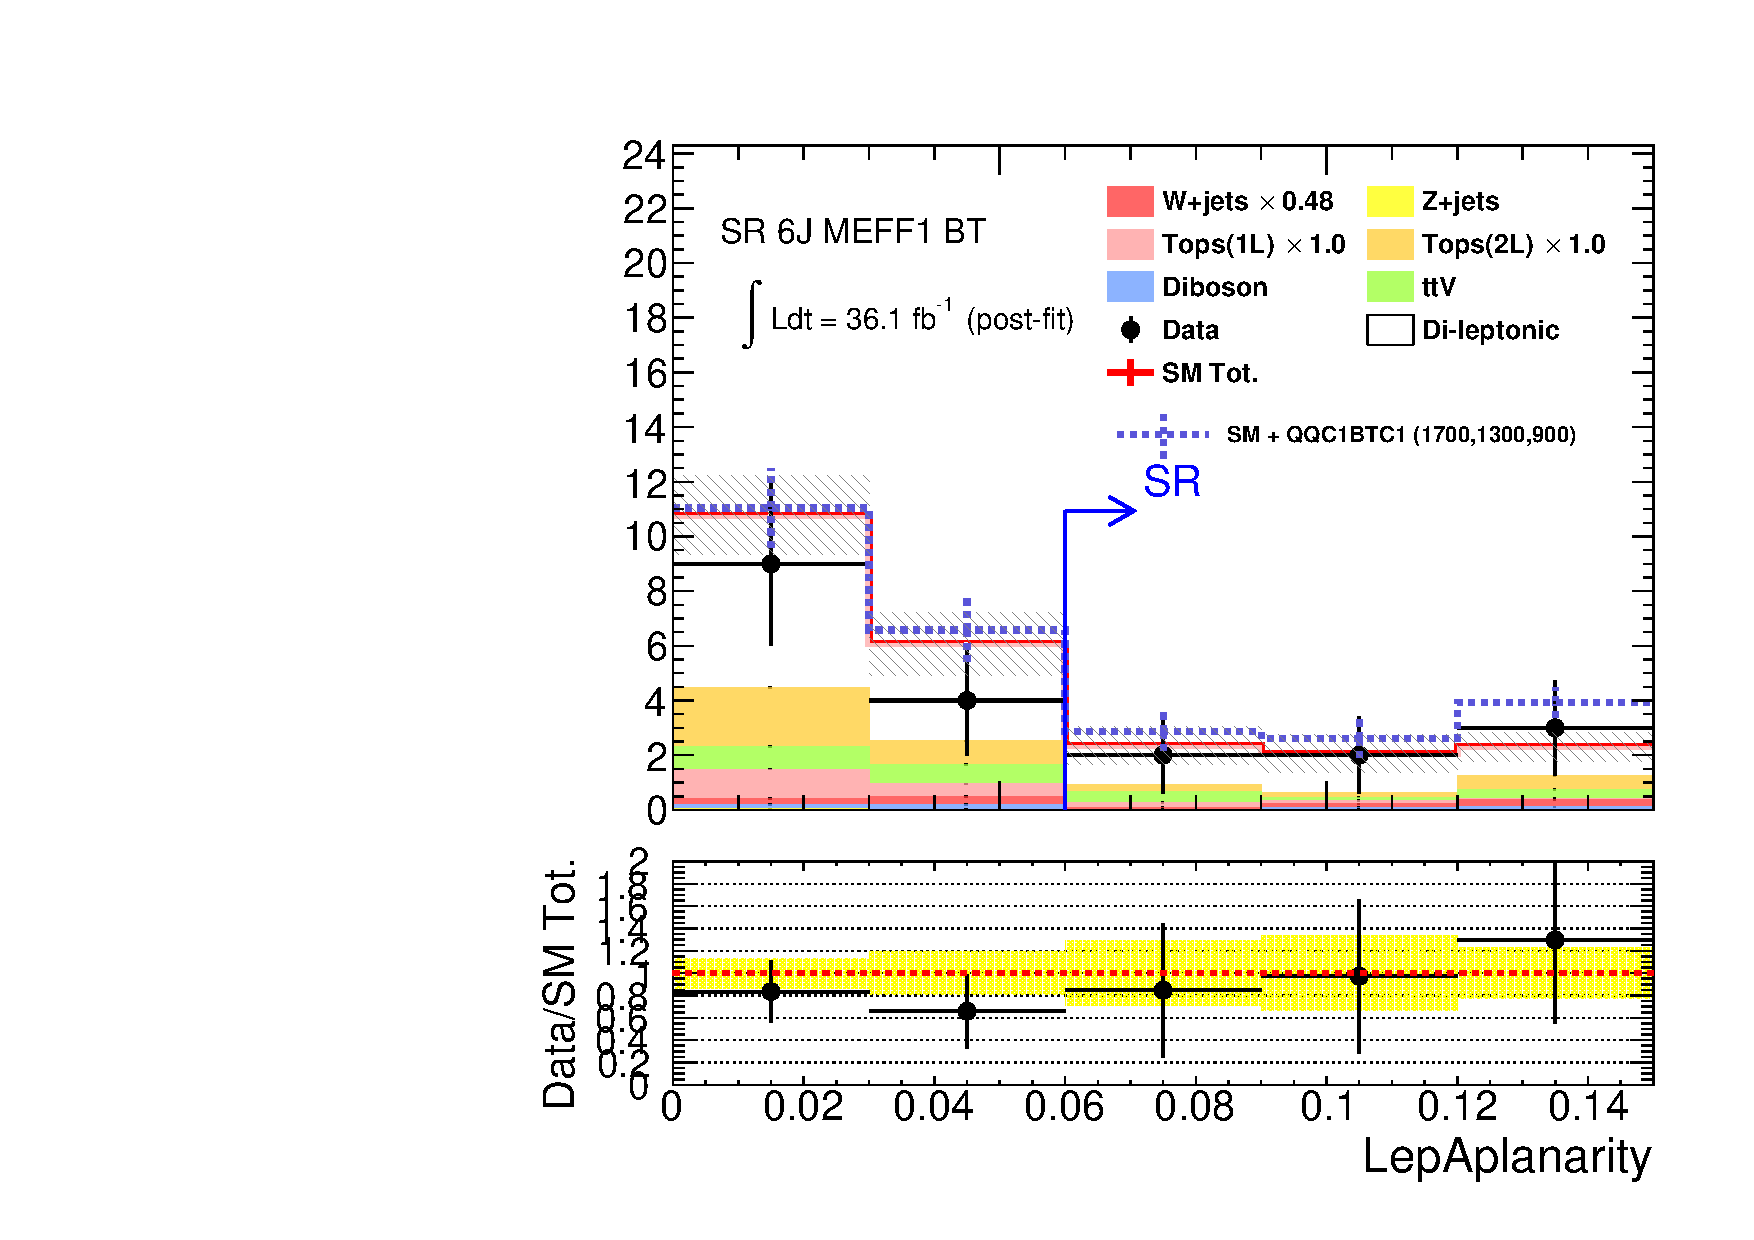
\includegraphics[width=0.41\textwidth]{figures/BGestimation/SRVRpostFit/LepAplanarity__SR6JMEFF1BT_no_LepAplanarity_postFit_2SFconfig_noYields_objRep.pdf}}
    \subfigure[]{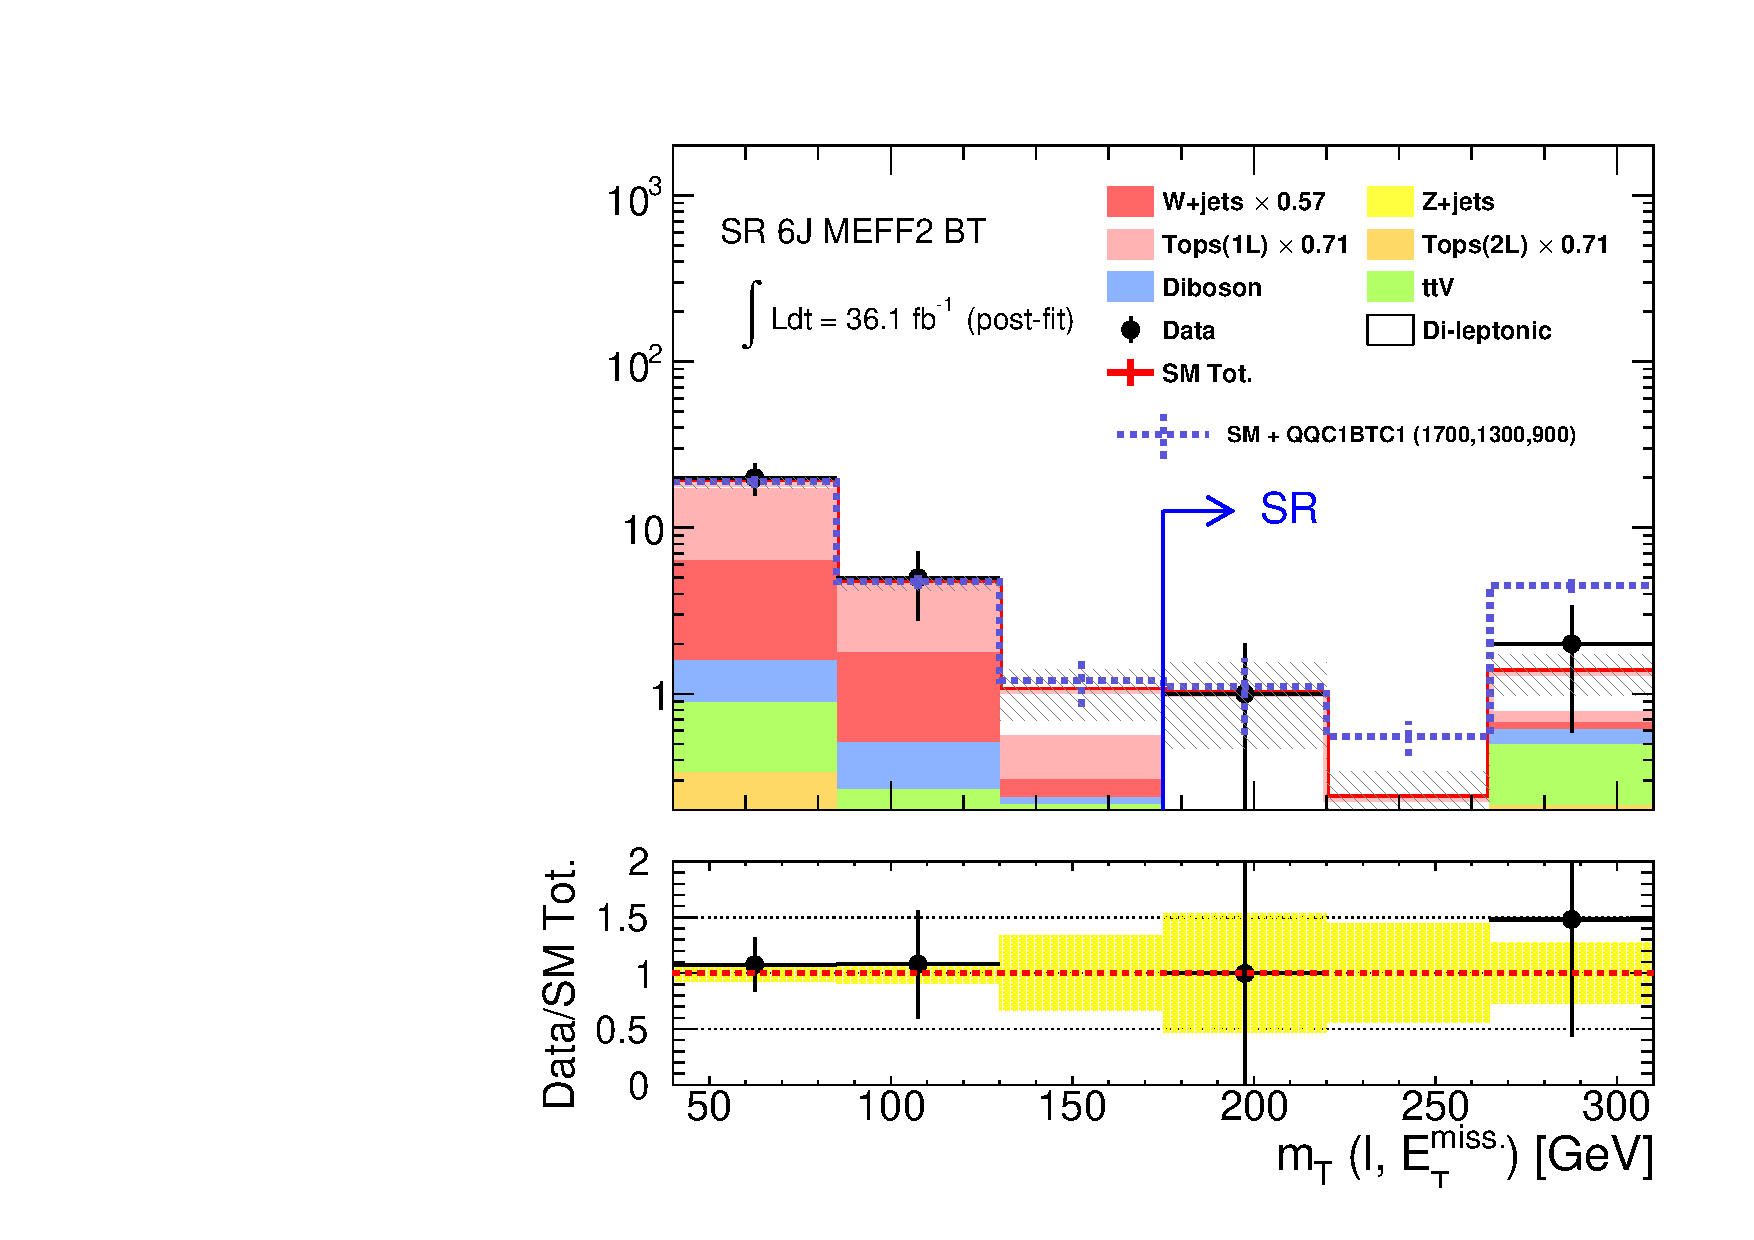
\includegraphics[width=0.41\textwidth]{figures/BGestimation/SRVRpostFit/mt__SR6JMEFF2BT_no_mt_postFit_2SFconfig_noYields_objRep.pdf}}
    \subfigure[]{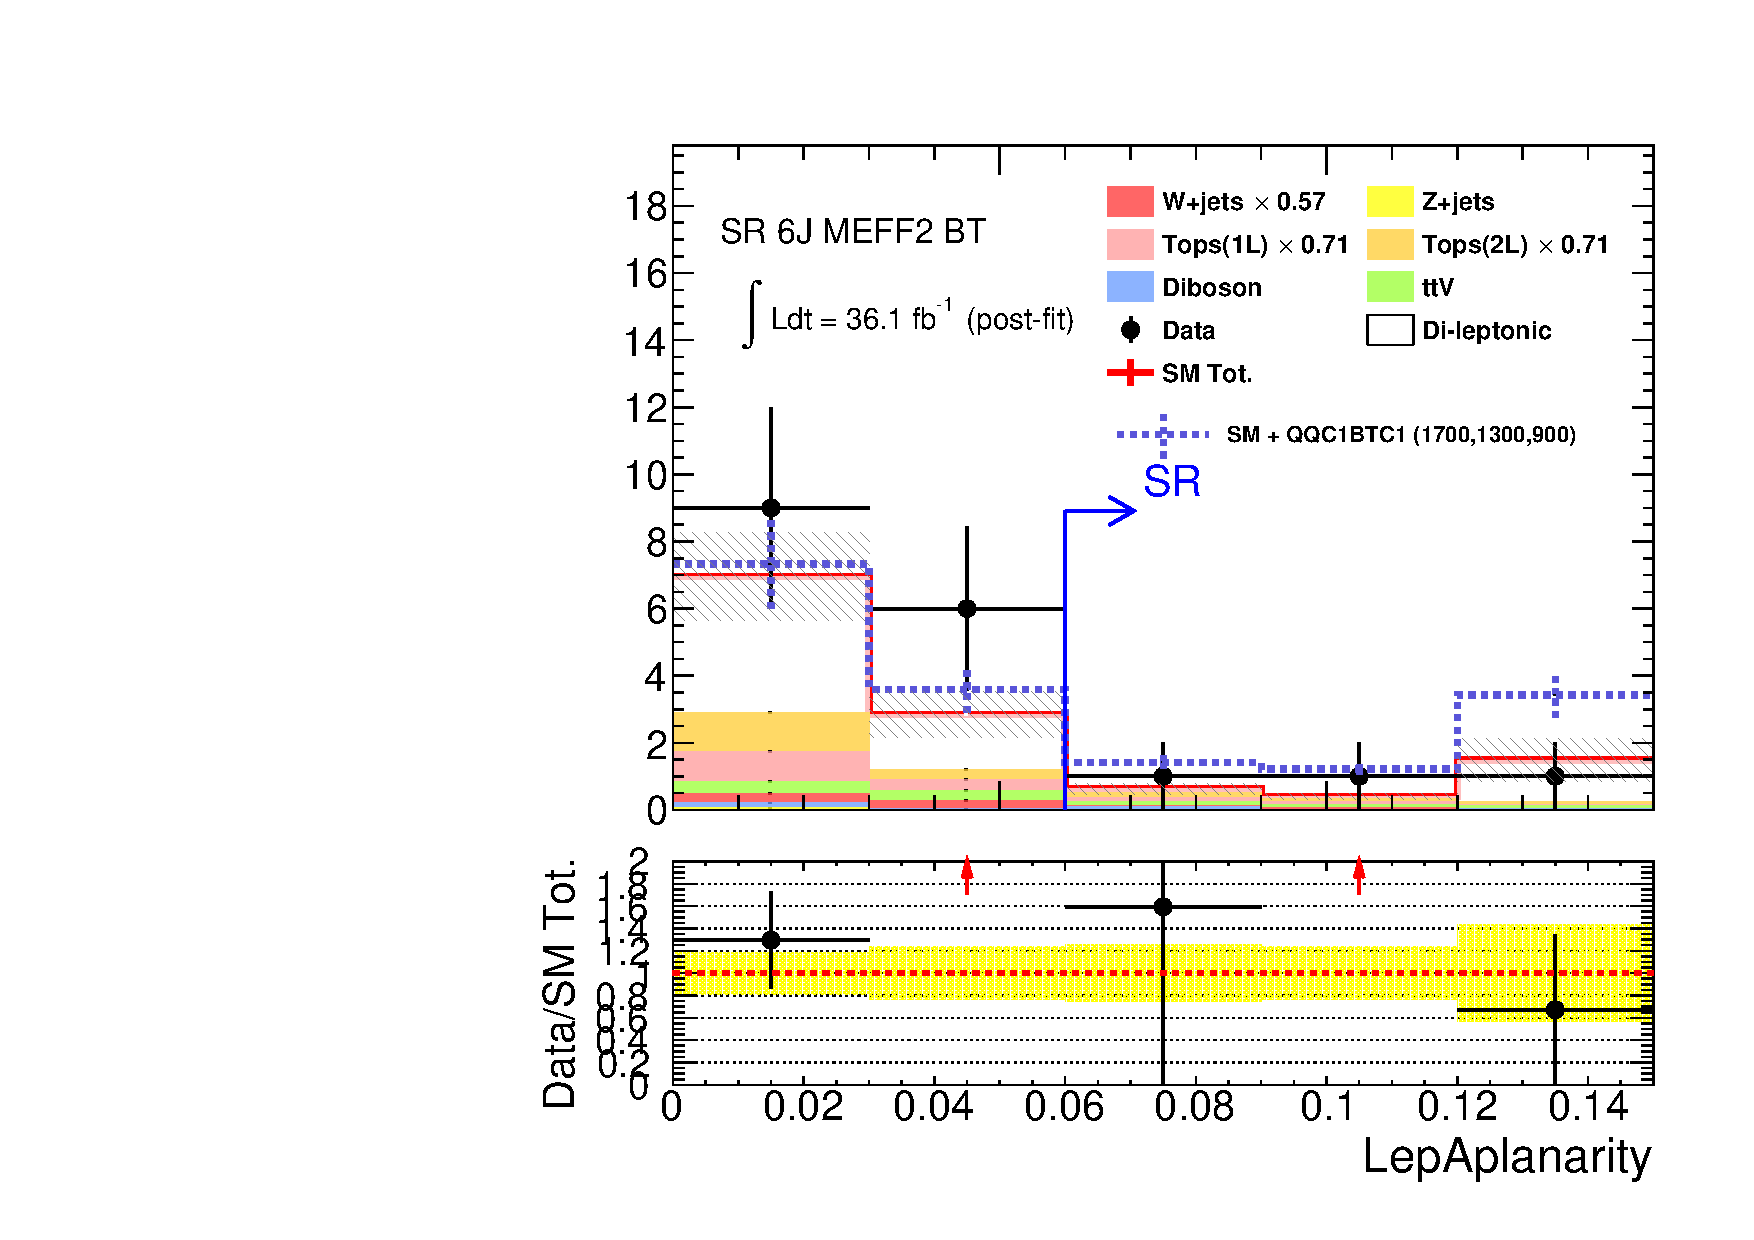
\includegraphics[width=0.41\textwidth]{figures/BGestimation/SRVRpostFit/LepAplanarity__SR6JMEFF2BT_no_LepAplanarity_postFit_2SFconfig_noYields_objRep.pdf}}
    \subfigure[]{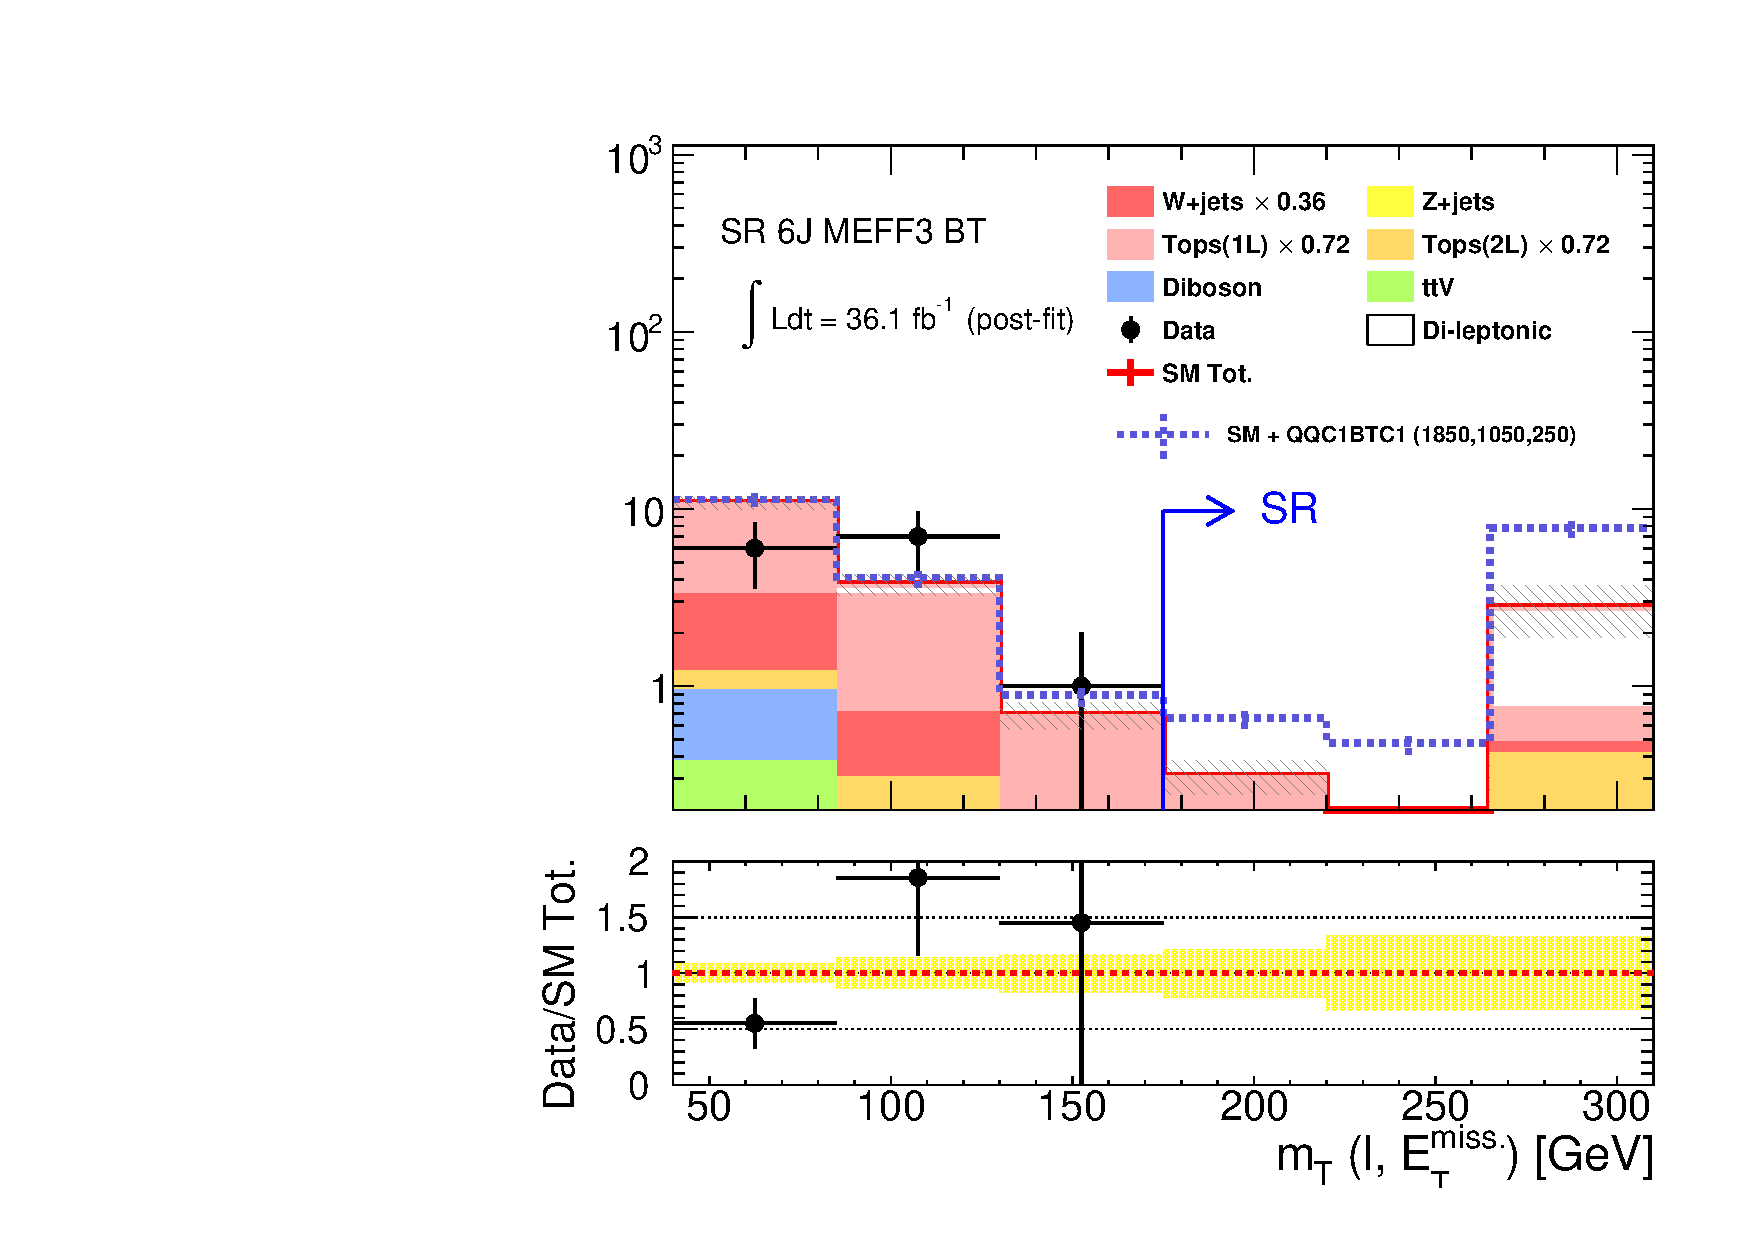
\includegraphics[width=0.41\textwidth]{figures/BGestimation/SRVRpostFit/mt__SR6JMEFF3BT_no_mt_postFit_2SFconfig_noYields_objRep.pdf}}
    \subfigure[]{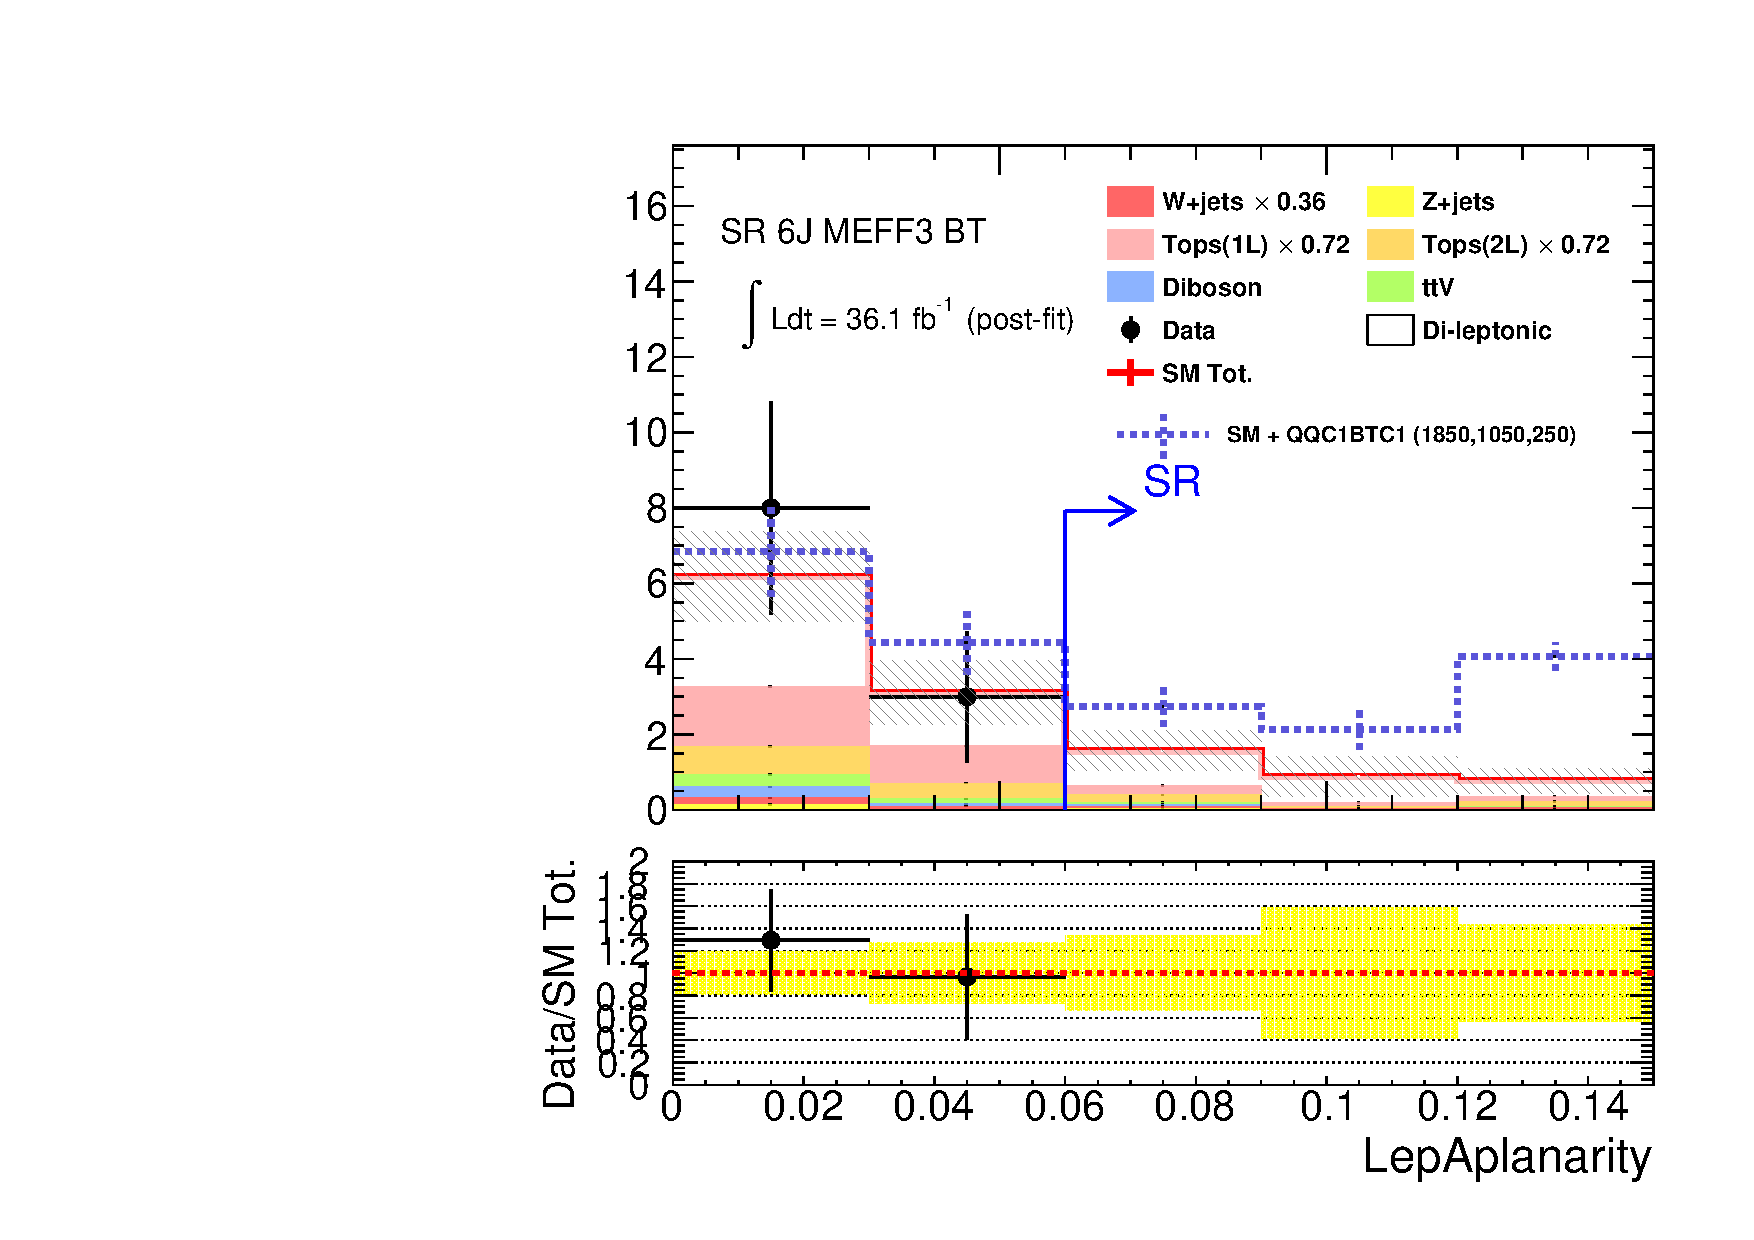
\includegraphics[width=0.41\textwidth]{figures/BGestimation/SRVRpostFit/LepAplanarity__SR6JMEFF3BT_no_LepAplanarity_postFit_2SFconfig_noYields_objRep.pdf}}
    \caption{
      Post-fit distruibution of (left) $\mt$, and (right) $\apl$.
      (a,b) SR 6J-$\meffIncFirst$ BT.
      (c,d) SR 6J-$\meffIncSecond$ BT.
      (e,f) SR 6J-$\meffIncThird$ BT.
      The yellow band in the bottom panel represents only statistical error. The overflow is included in the highest bin.  
      \label{fig::BGestimation::SRVRpostFit::SR6JBT}
    }
\end{figure}

\clearpage
\begin{figure}[h]
  \centering
    \subfigure[]{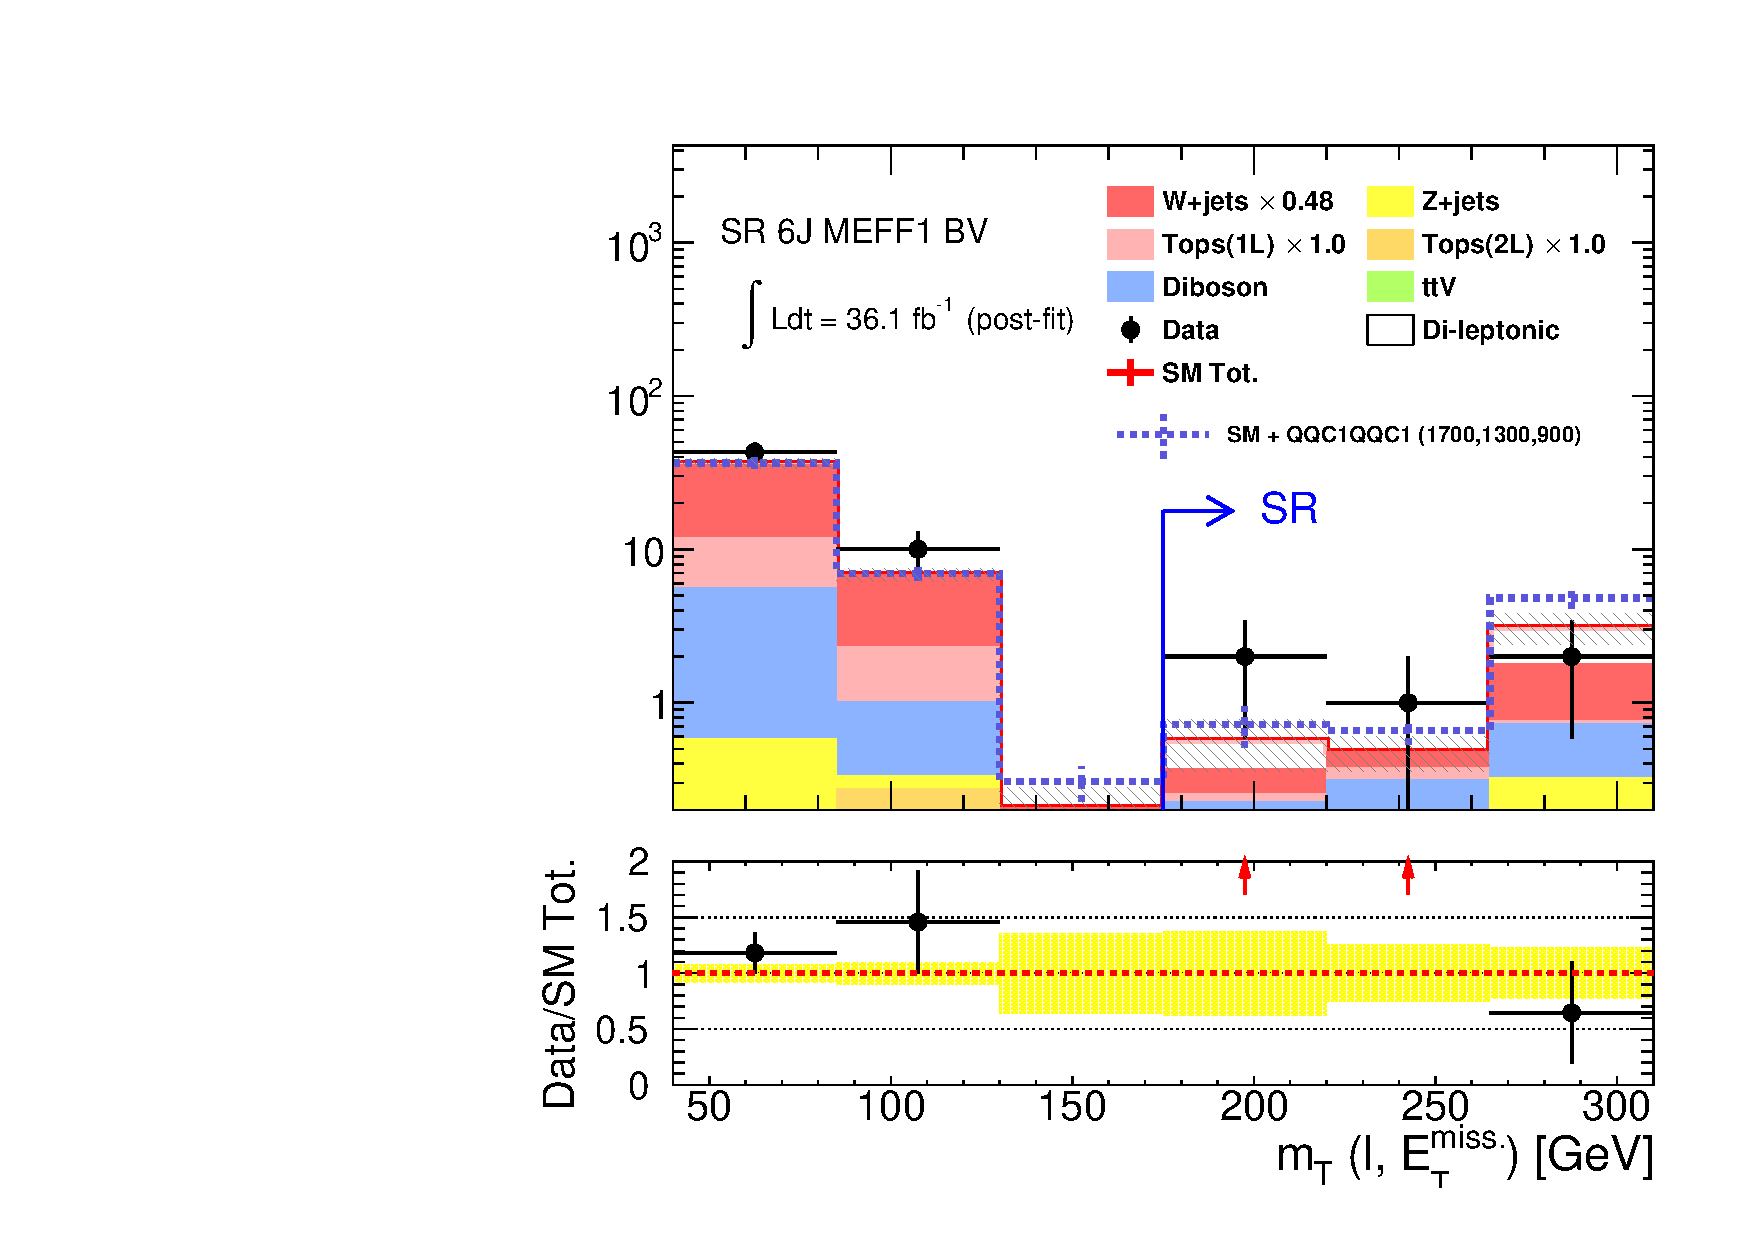
\includegraphics[width=0.41\textwidth]{figures/BGestimation/SRVRpostFit/mt__SR6JMEFF1BV_no_mt_postFit_2SFconfig_noYields_objRep.pdf}}
    \subfigure[]{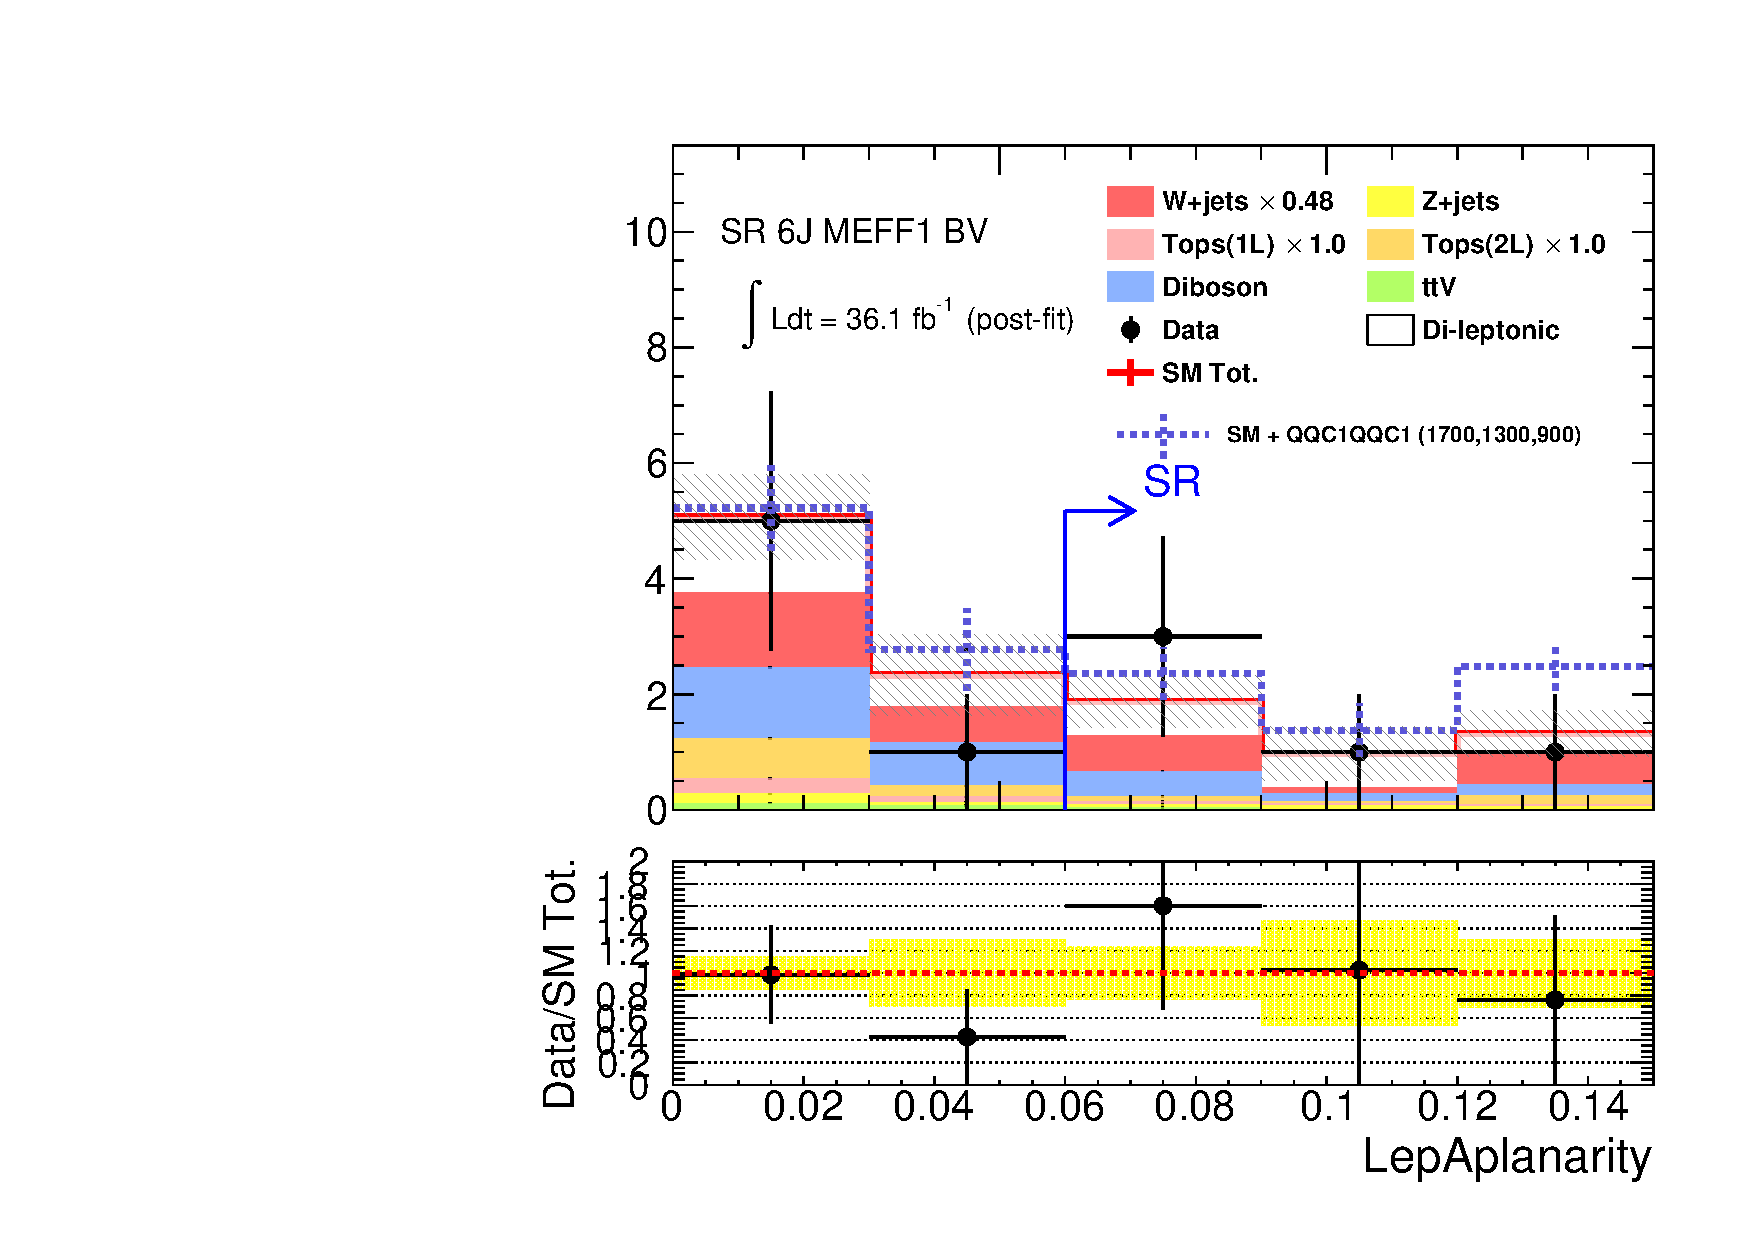
\includegraphics[width=0.41\textwidth]{figures/BGestimation/SRVRpostFit/LepAplanarity__SR6JMEFF1BV_no_LepAplanarity_postFit_2SFconfig_noYields_objRep.pdf}}
    \subfigure[]{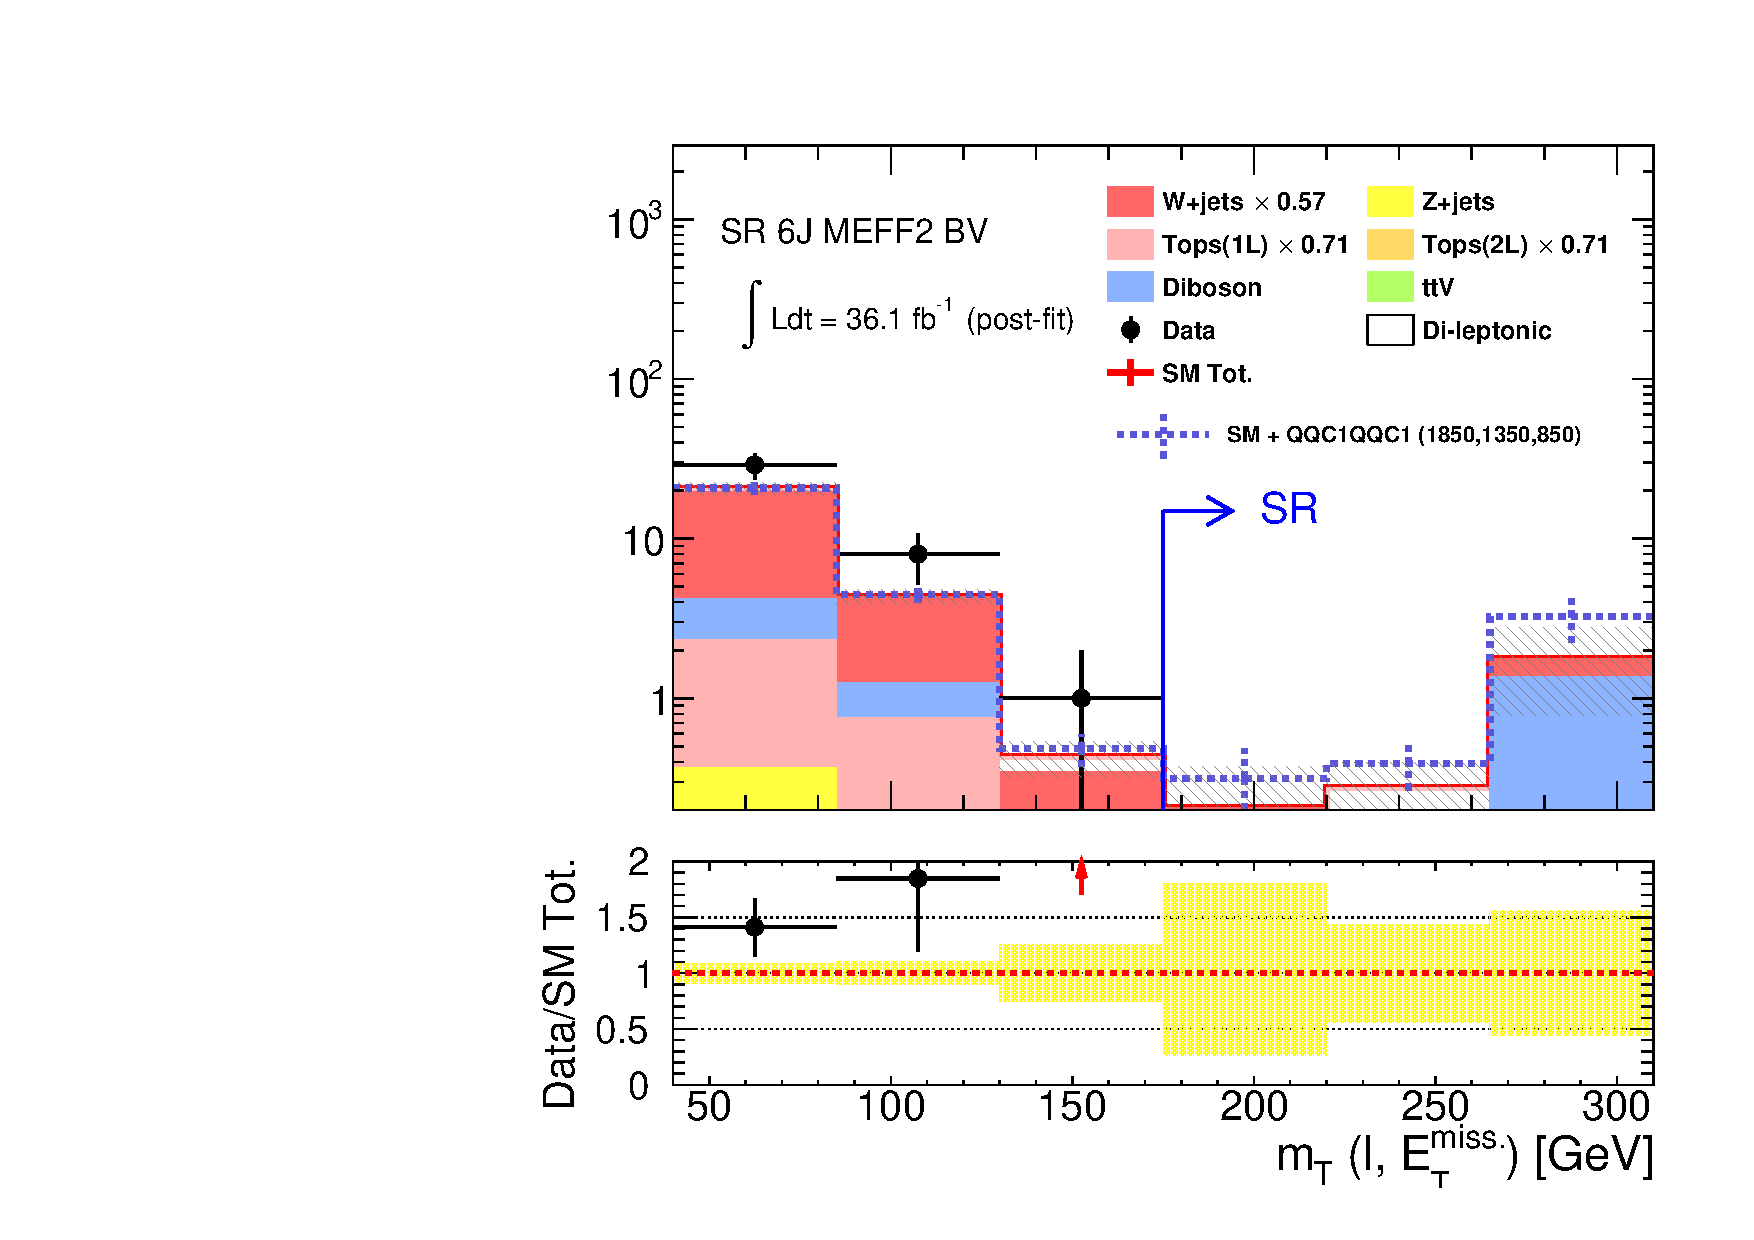
\includegraphics[width=0.41\textwidth]{figures/BGestimation/SRVRpostFit/mt__SR6JMEFF2BV_no_mt_postFit_2SFconfig_noYields_objRep.pdf}}
    \subfigure[]{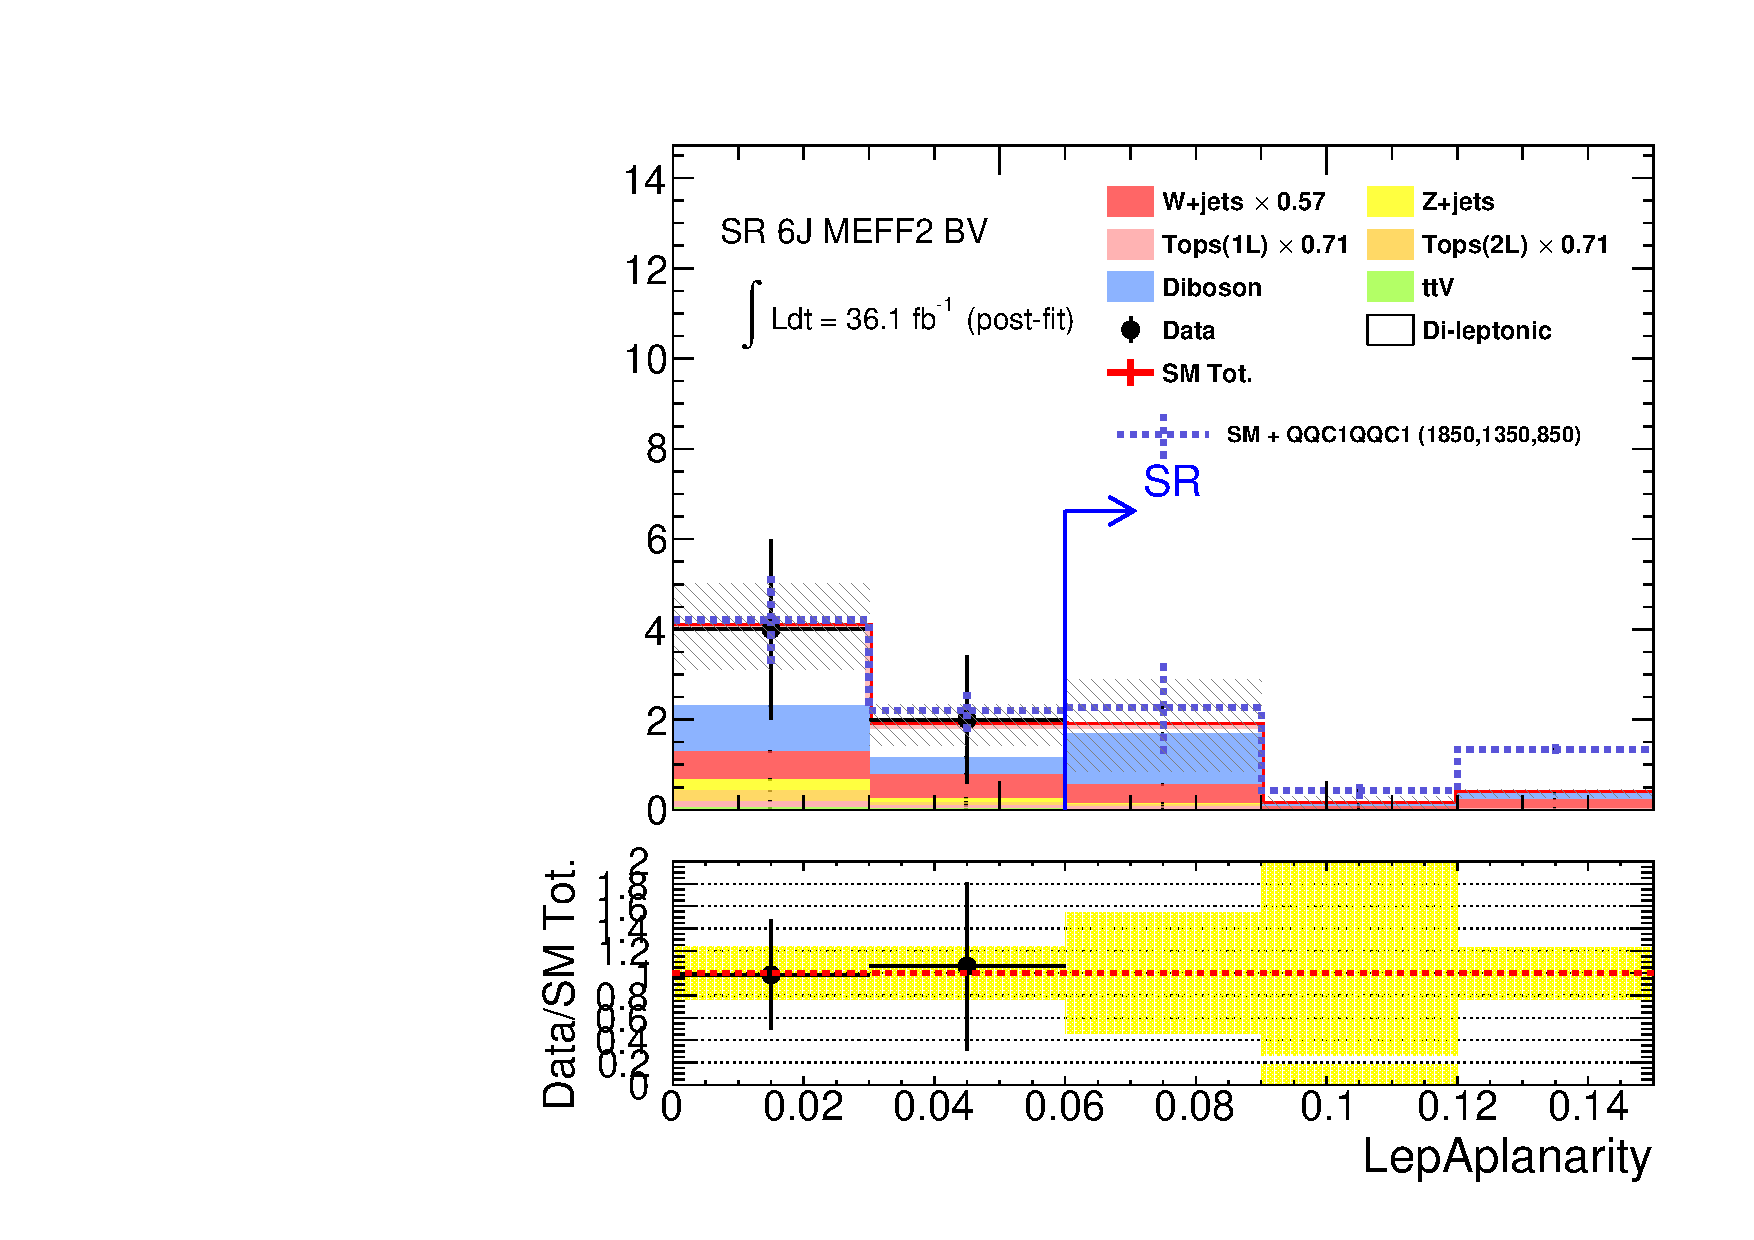
\includegraphics[width=0.41\textwidth]{figures/BGestimation/SRVRpostFit/LepAplanarity__SR6JMEFF2BV_no_LepAplanarity_postFit_2SFconfig_noYields_objRep.pdf}}
    \subfigure[]{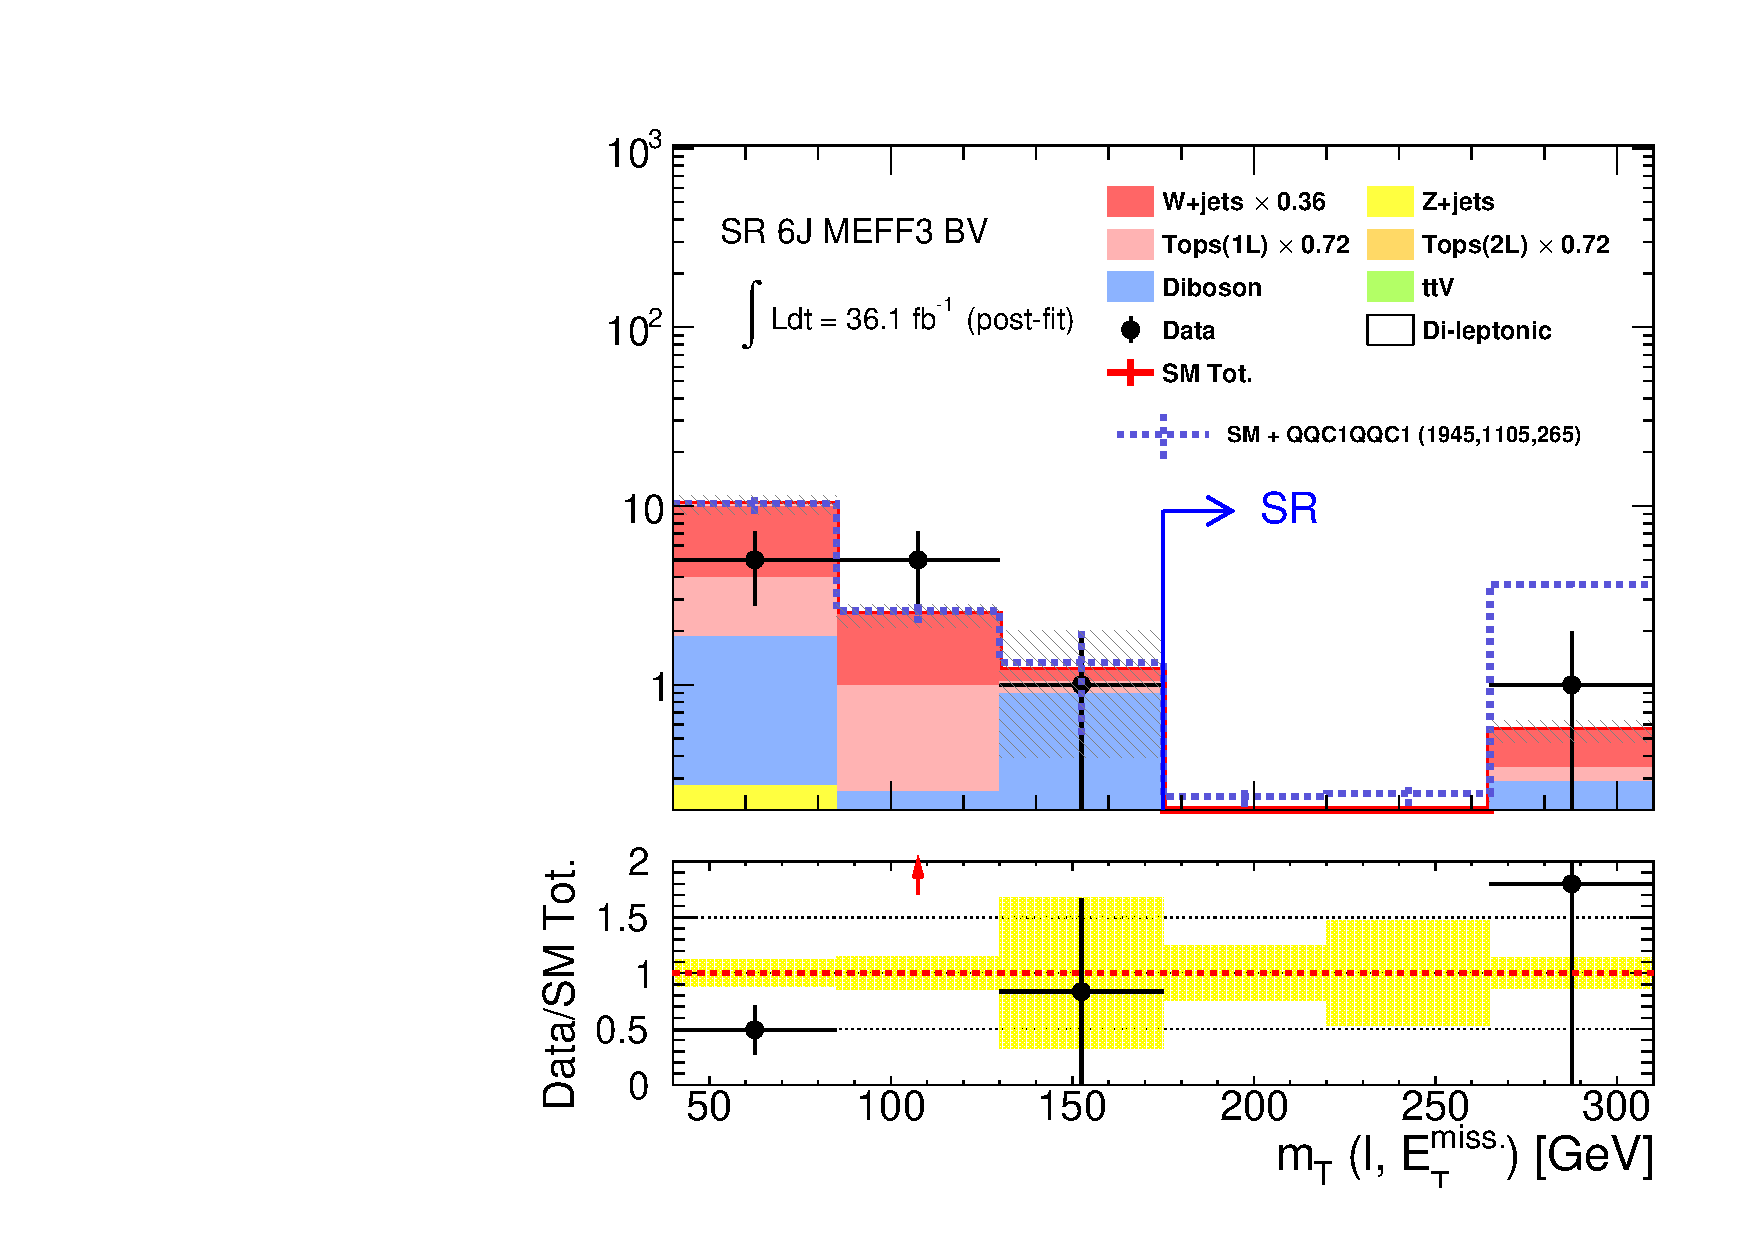
\includegraphics[width=0.41\textwidth]{figures/BGestimation/SRVRpostFit/mt__SR6JMEFF3BV_no_mt_postFit_2SFconfig_noYields_objRep.pdf}}
    \subfigure[]{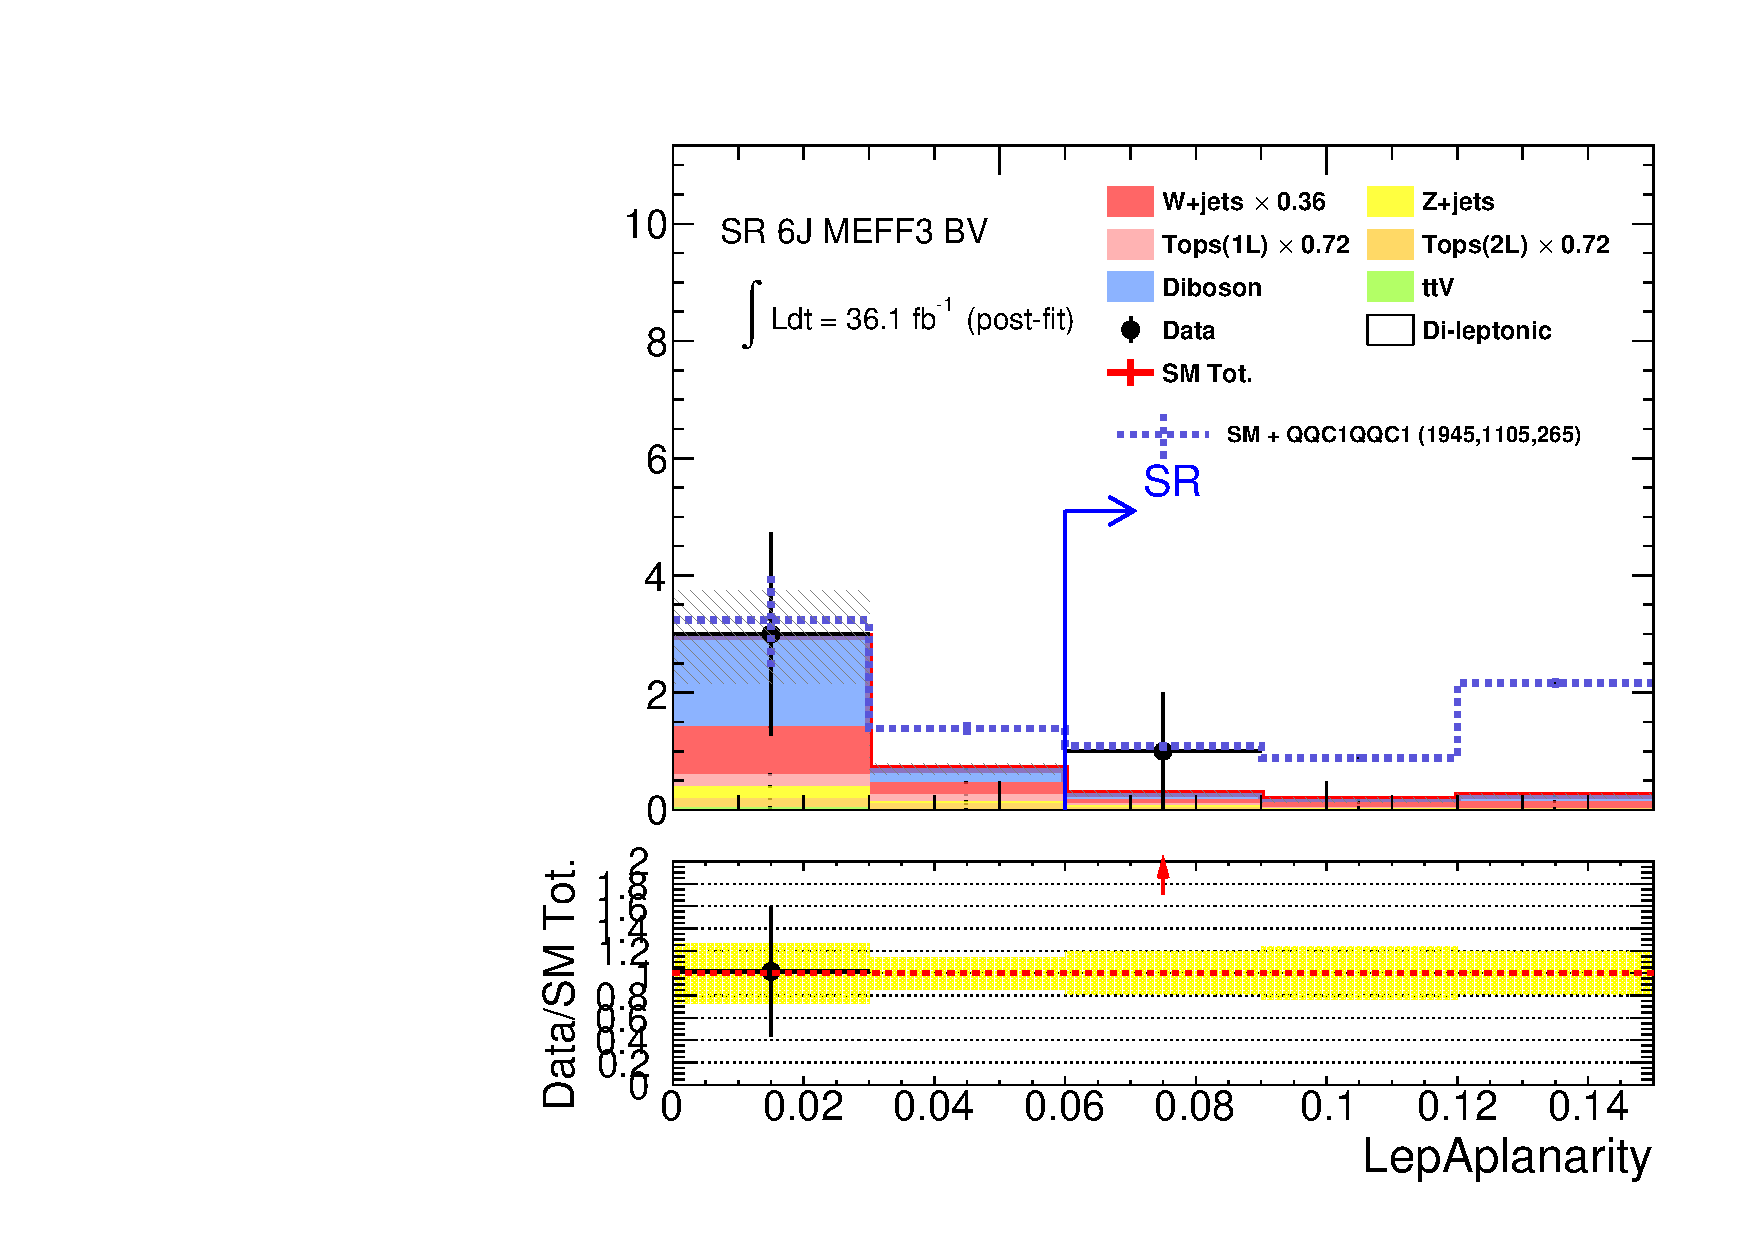
\includegraphics[width=0.41\textwidth]{figures/BGestimation/SRVRpostFit/LepAplanarity__SR6JMEFF3BV_no_LepAplanarity_postFit_2SFconfig_noYields_objRep.pdf}}
    \caption{
      Post-fit distruibution of (left) $\mt$, and (right) $\apl$.
      (a,b) SR 6J-$\meffIncFirst$ BV.
      (c,d) SR 6J-$\meffIncSecond$ BV.
      (e,f) SR 6J-$\meffIncThird$ BV.
      The yellow band in the bottom panel represents only statistical error. The overflow is included in the highest bin.  
      \label{fig::BGestimation::SRVRpostFit::SR6JBV}
    }
\end{figure}
%----------------------------------


\clearpage
% -------------- varx ---------
\begin{figure}[h]
  \centering
    \subfigure[]{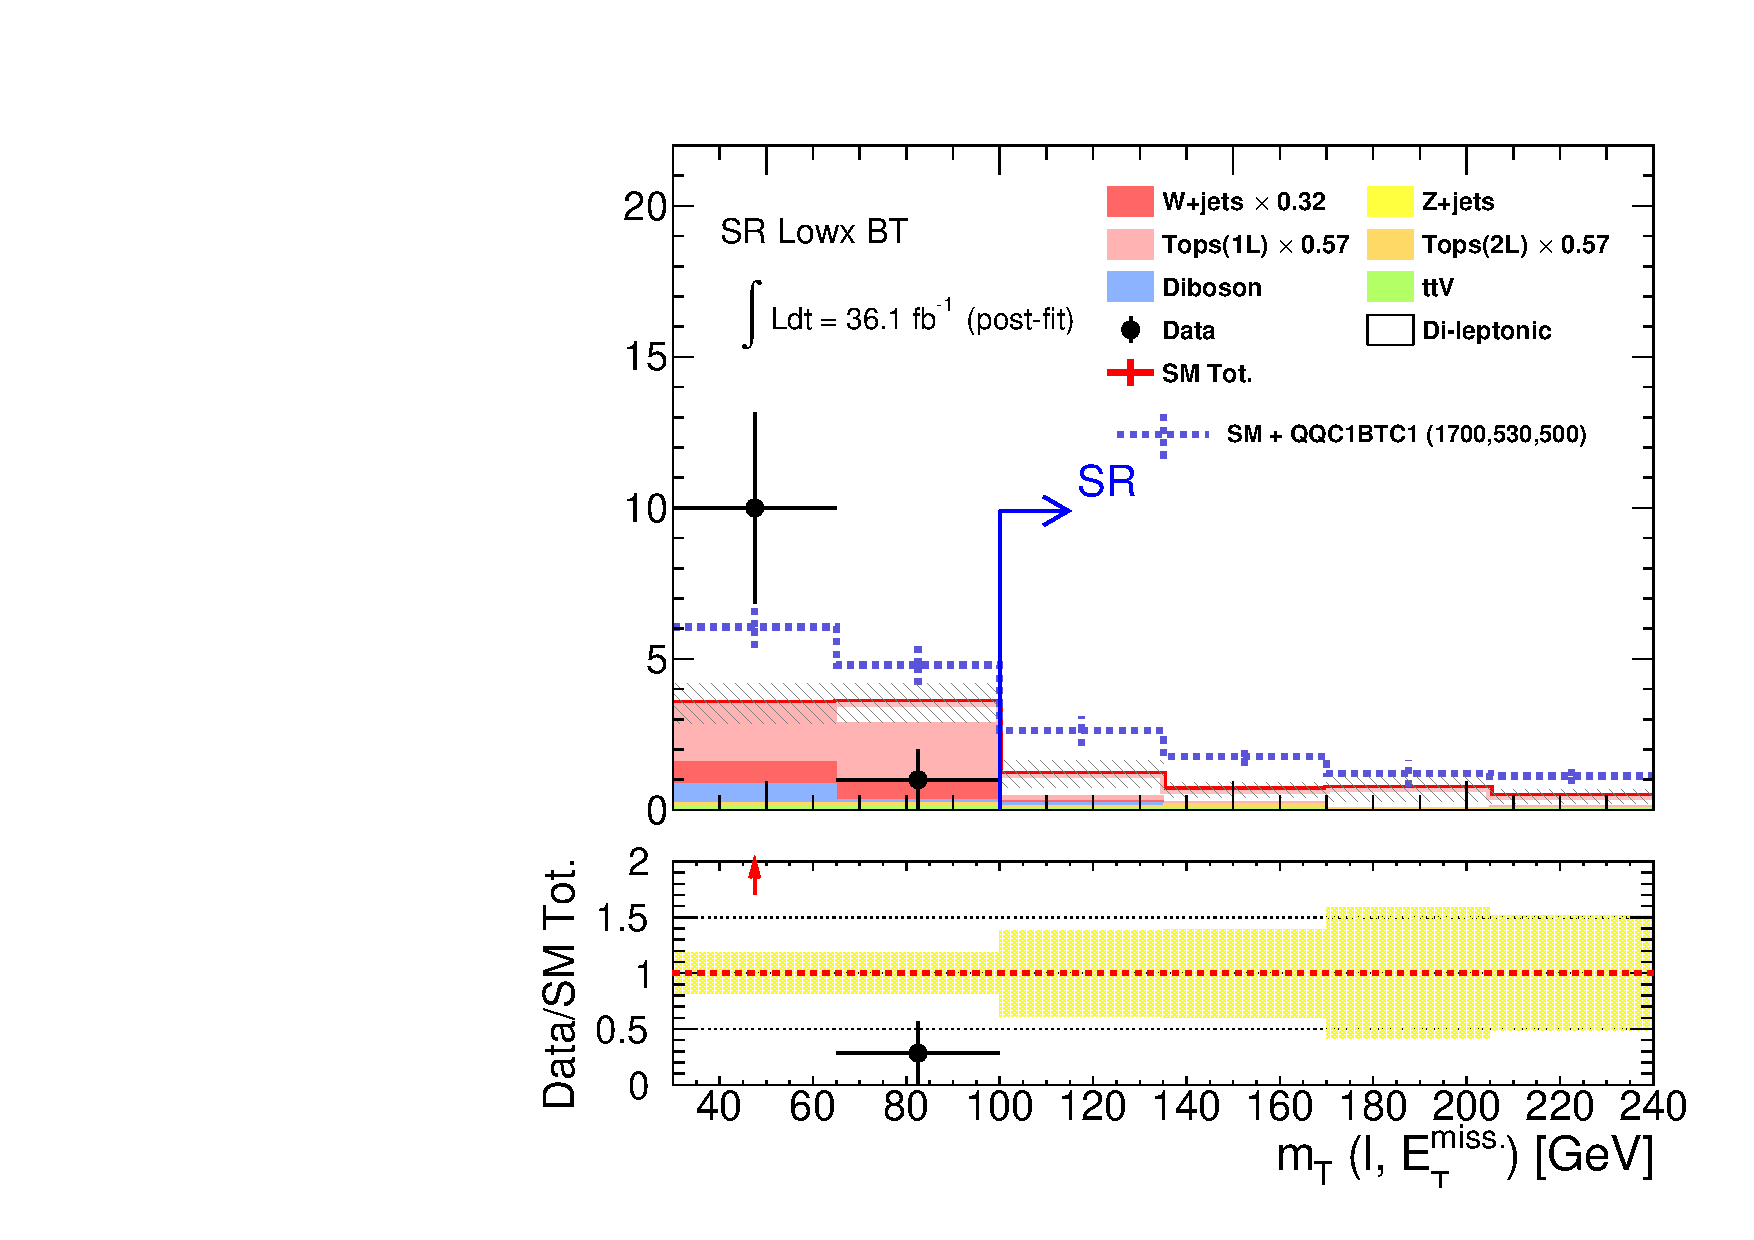
\includegraphics[width=0.41\textwidth]{figures/BGestimation/SRVRpostFit/mt__SRLowxBT_no_mt_postFit_2SFconfig_noYields_objRep.pdf}}
    \subfigure[]{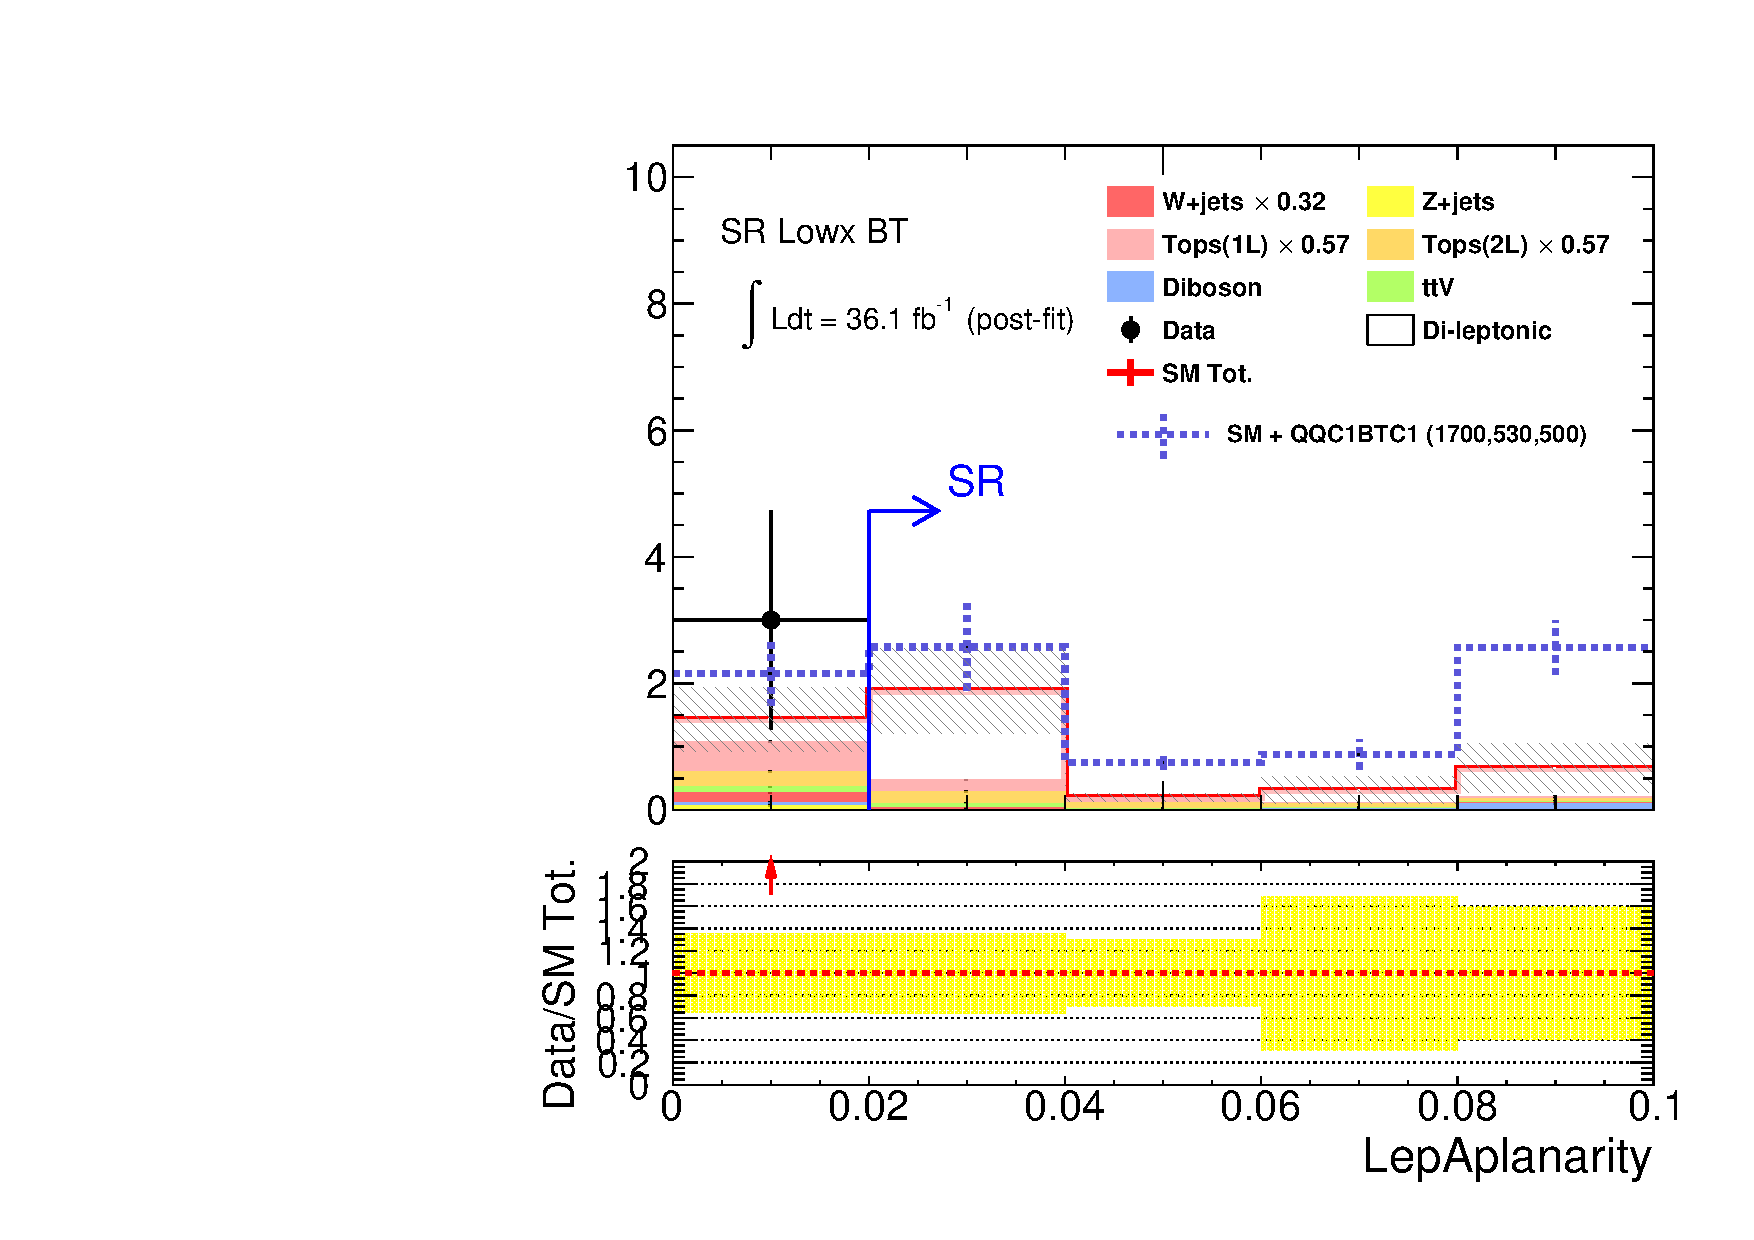
\includegraphics[width=0.41\textwidth]{figures/BGestimation/SRVRpostFit/LepAplanarity__SRLowxBT_no_LepAplanarity_postFit_2SFconfig_noYields_objRep.pdf}}
    \subfigure[]{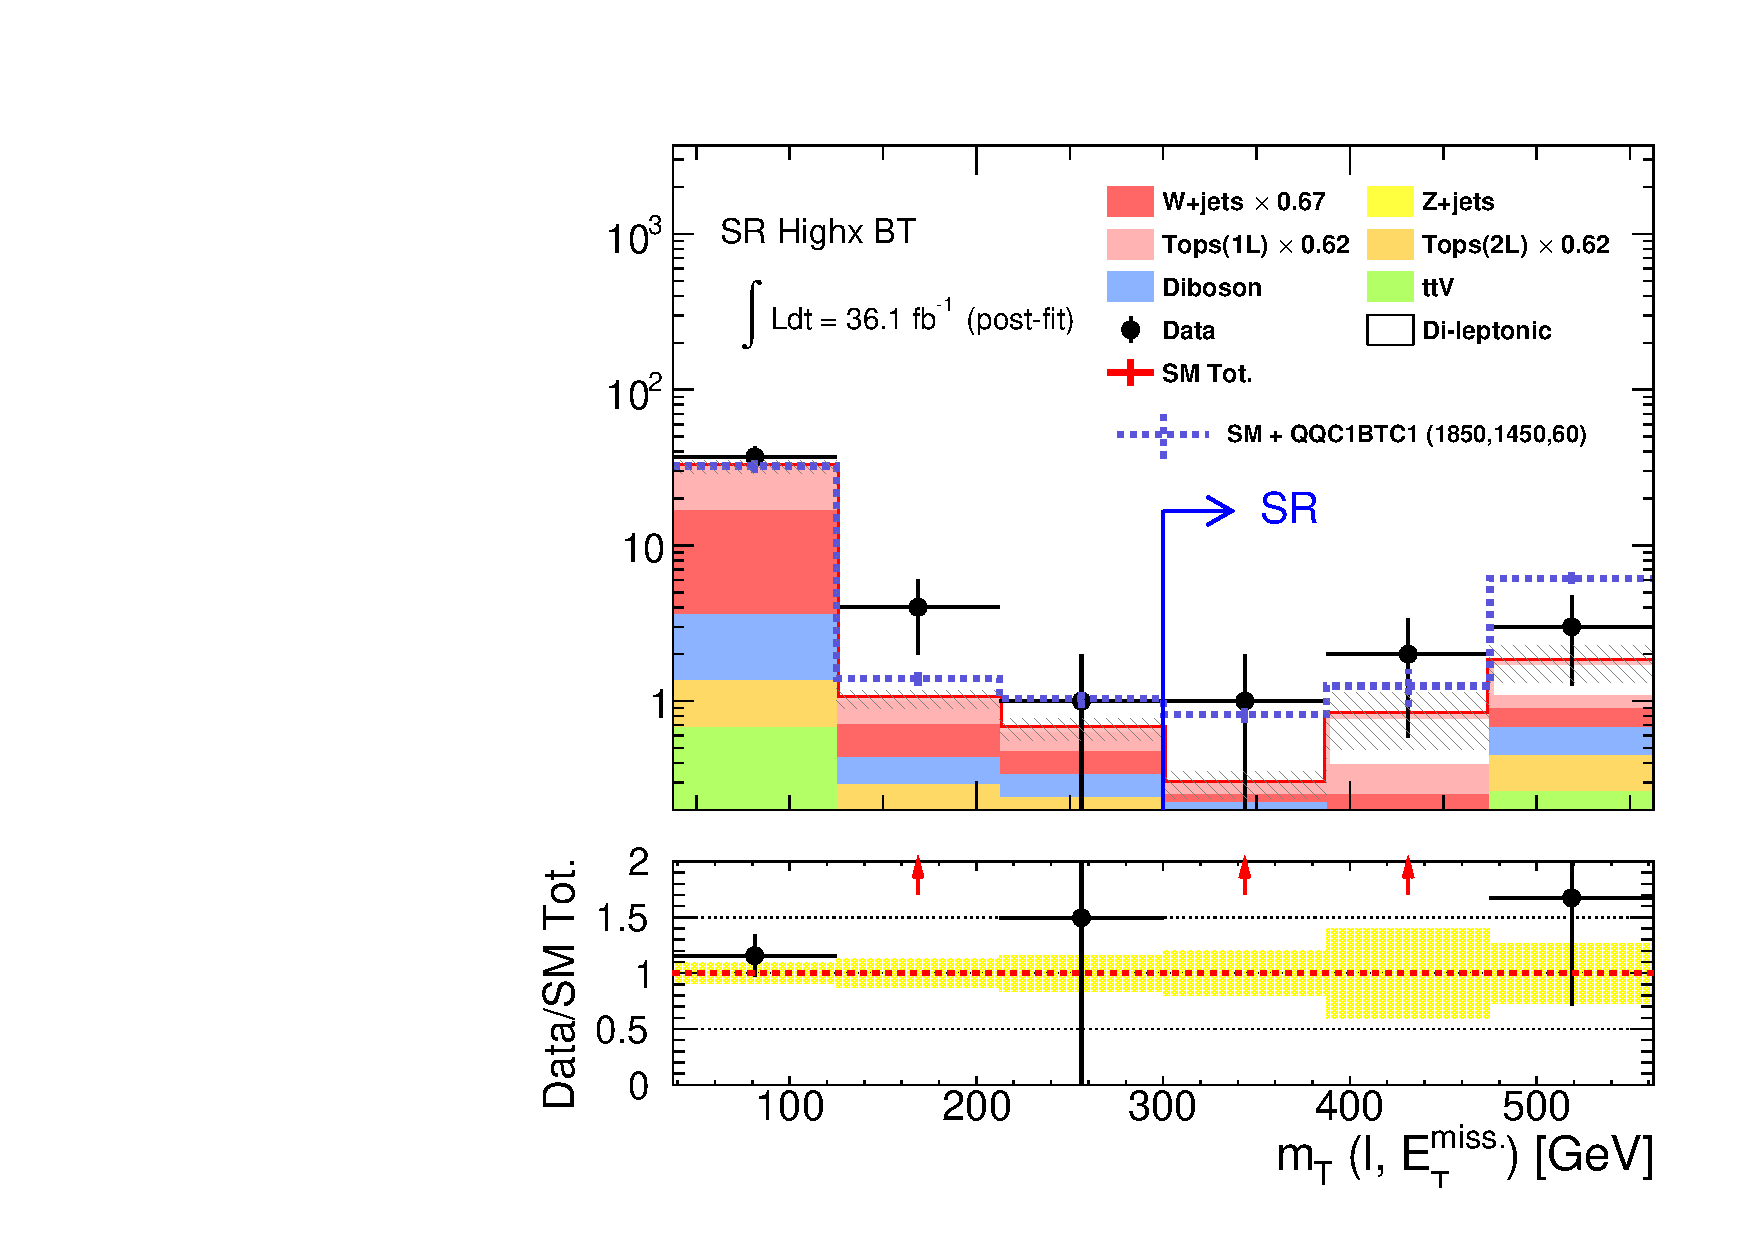
\includegraphics[width=0.41\textwidth]{figures/BGestimation/SRVRpostFit/mt__SRHighxBT_no_mt_postFit_2SFconfig_noYields_objRep.pdf}}
    \subfigure[]{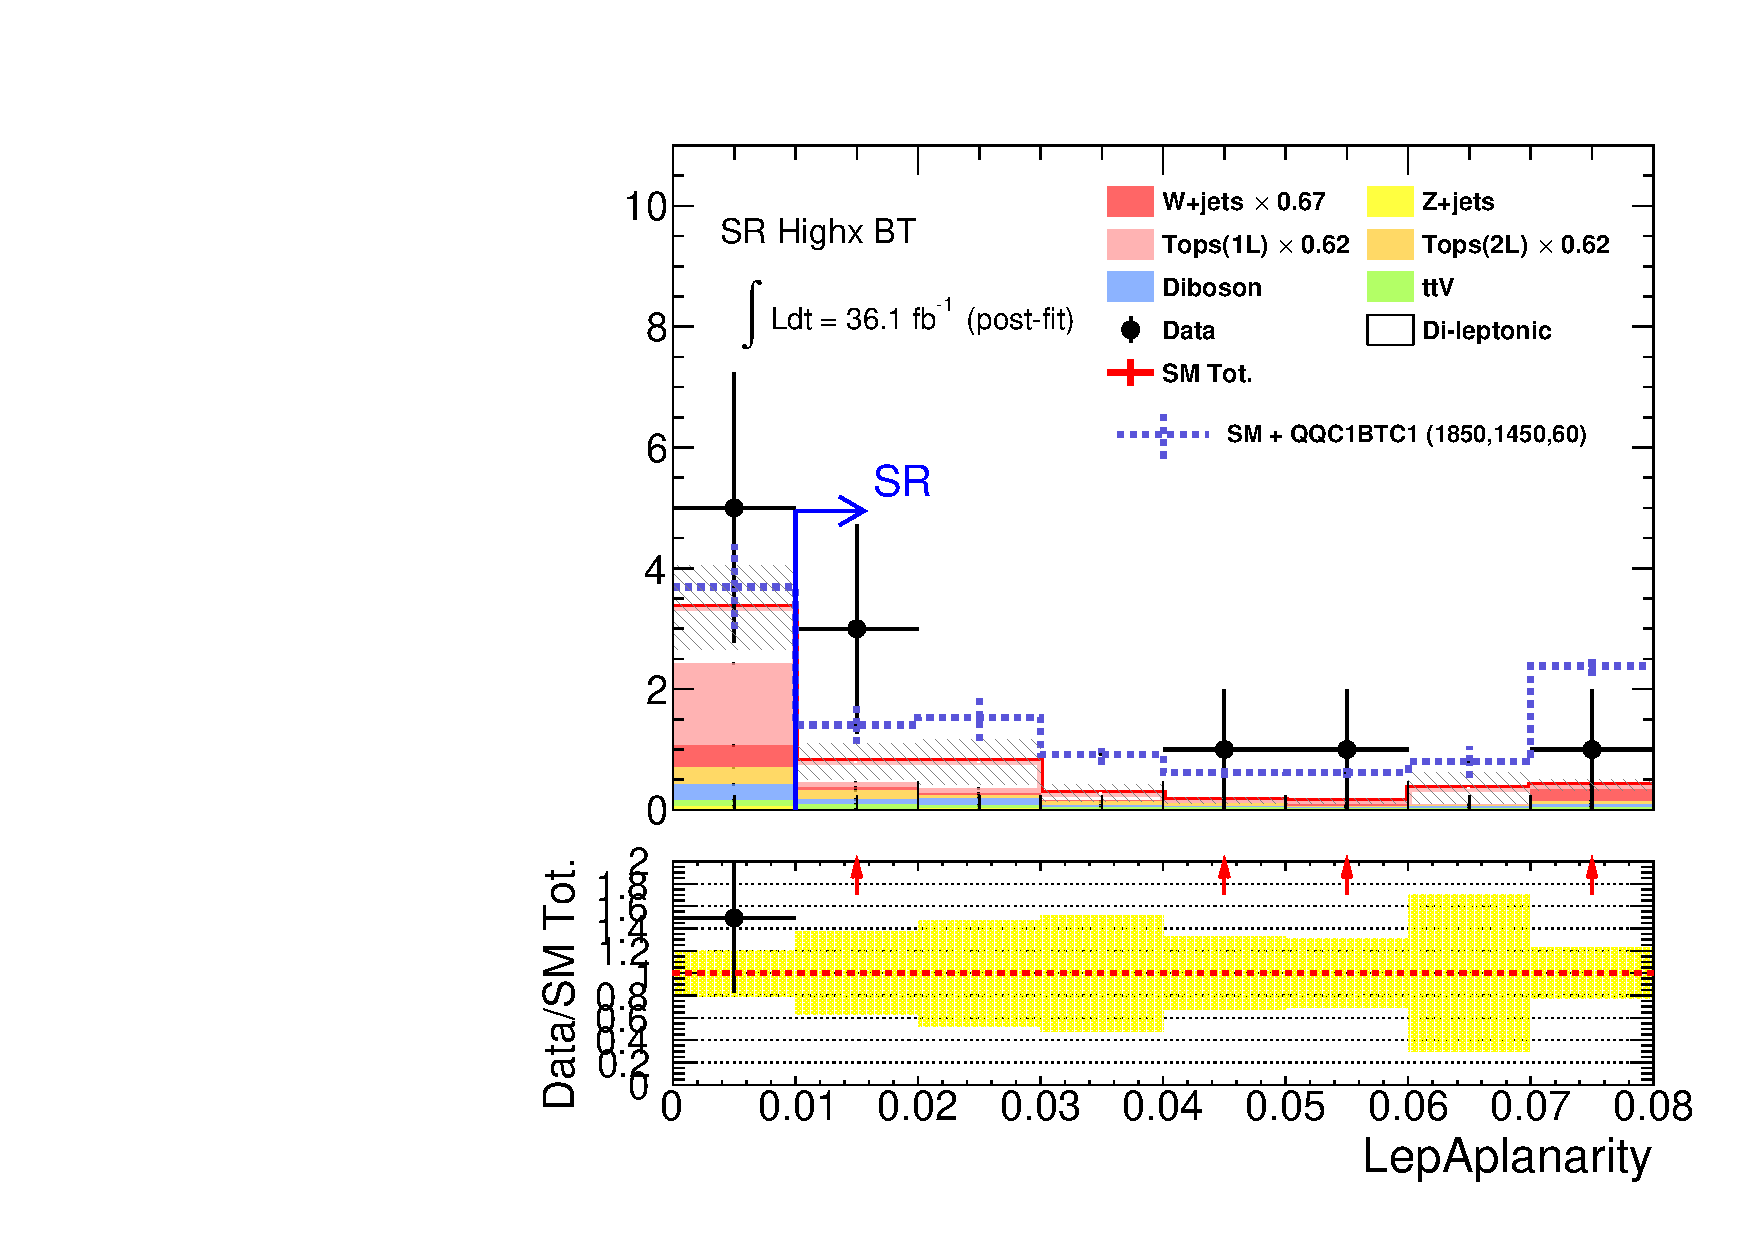
\includegraphics[width=0.41\textwidth]{figures/BGestimation/SRVRpostFit/LepAplanarity__SRHighxBT_no_LepAplanarity_postFit_2SFconfig_noYields_objRep.pdf}}
   \caption{   
     Post-fit distruibution of (left) $\mt$ and (right) $\apl$.
     (a,b) SR Low-x BT.
     (c,d) SR High-x BT.
     The yellow band in the bottom panel represents only statistical error. The overflow is included in the highest bin.  
     \label{fig::BGestimation::SRVRpostFit::SRVarxBT}
   }
\end{figure}

\clearpage
\begin{figure}[h]
  \centering
    \subfigure[]{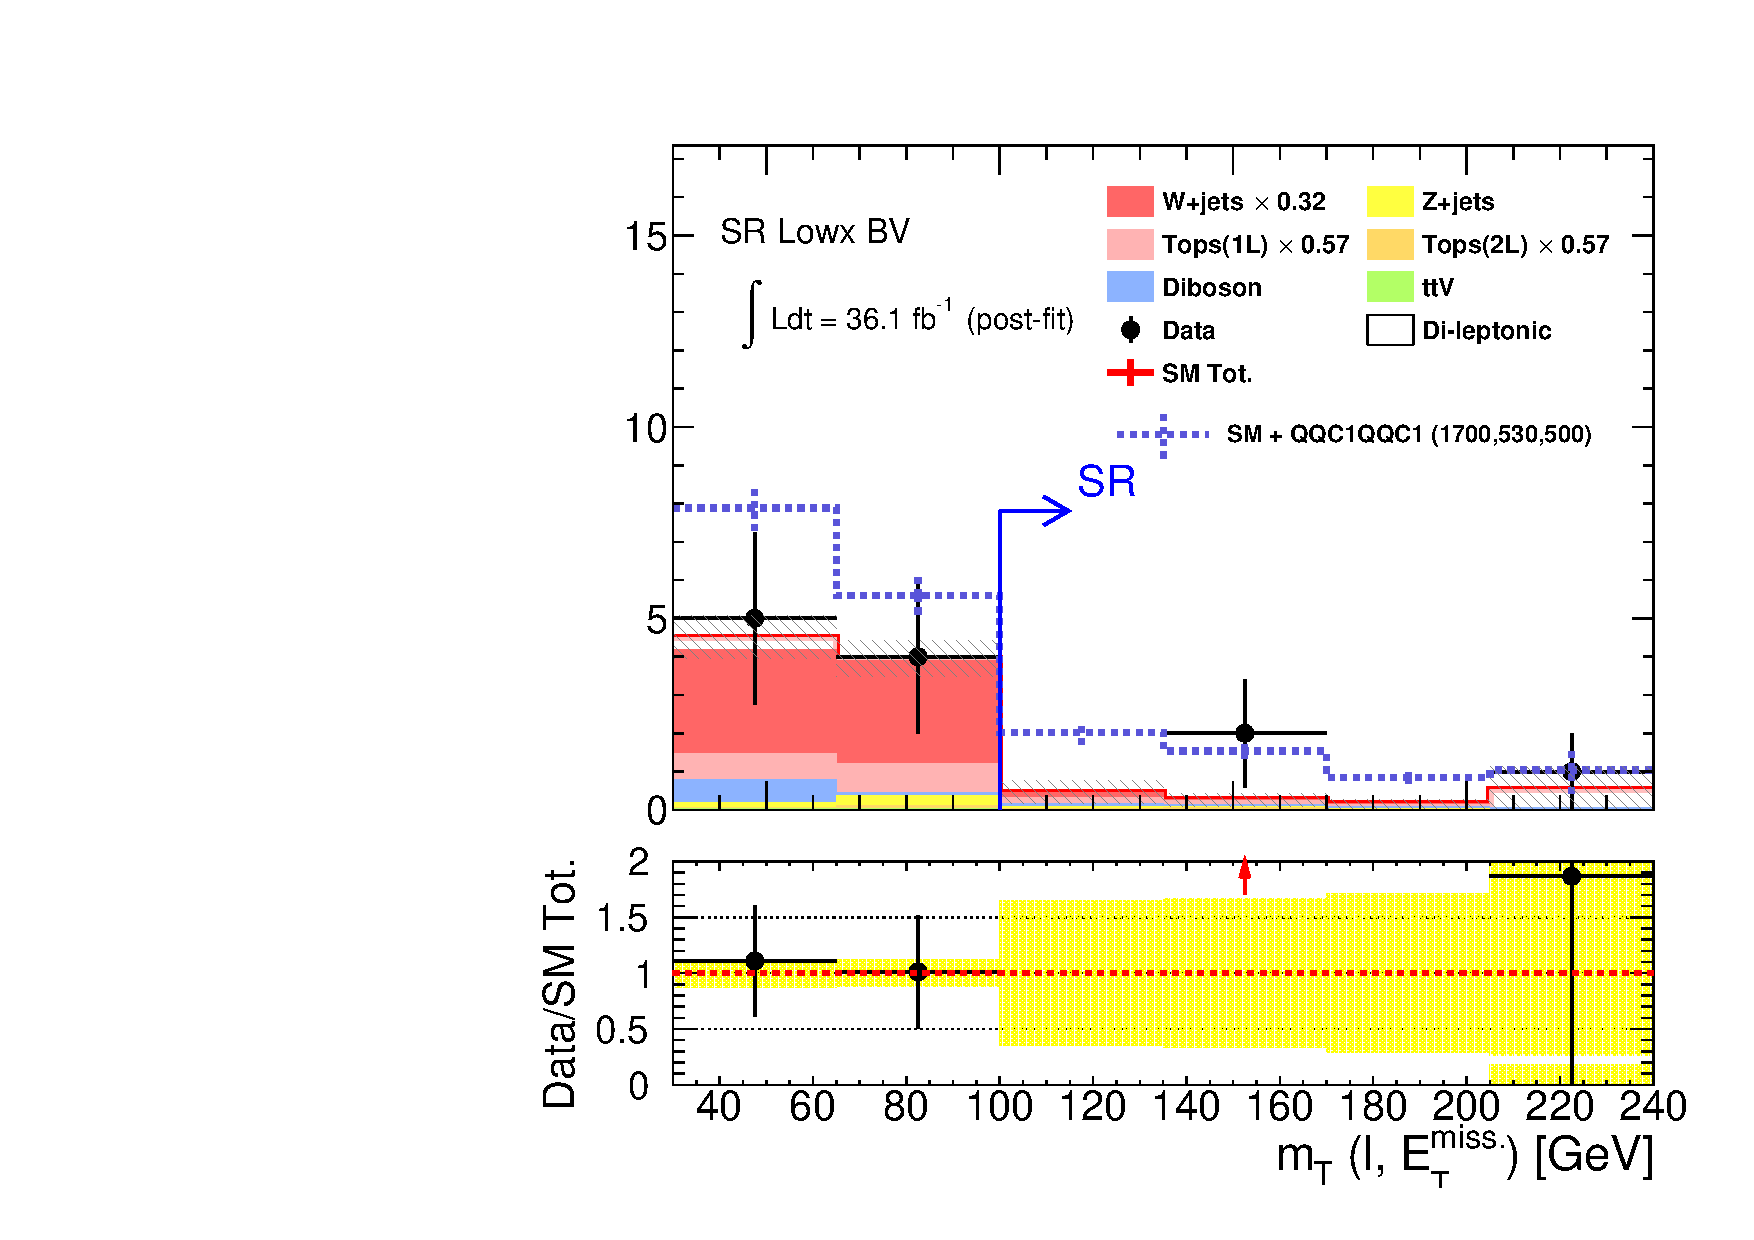
\includegraphics[width=0.41\textwidth]{figures/BGestimation/SRVRpostFit/mt__SRLowxBV_no_mt_postFit_2SFconfig_noYields_objRep.pdf}}
    \subfigure[]{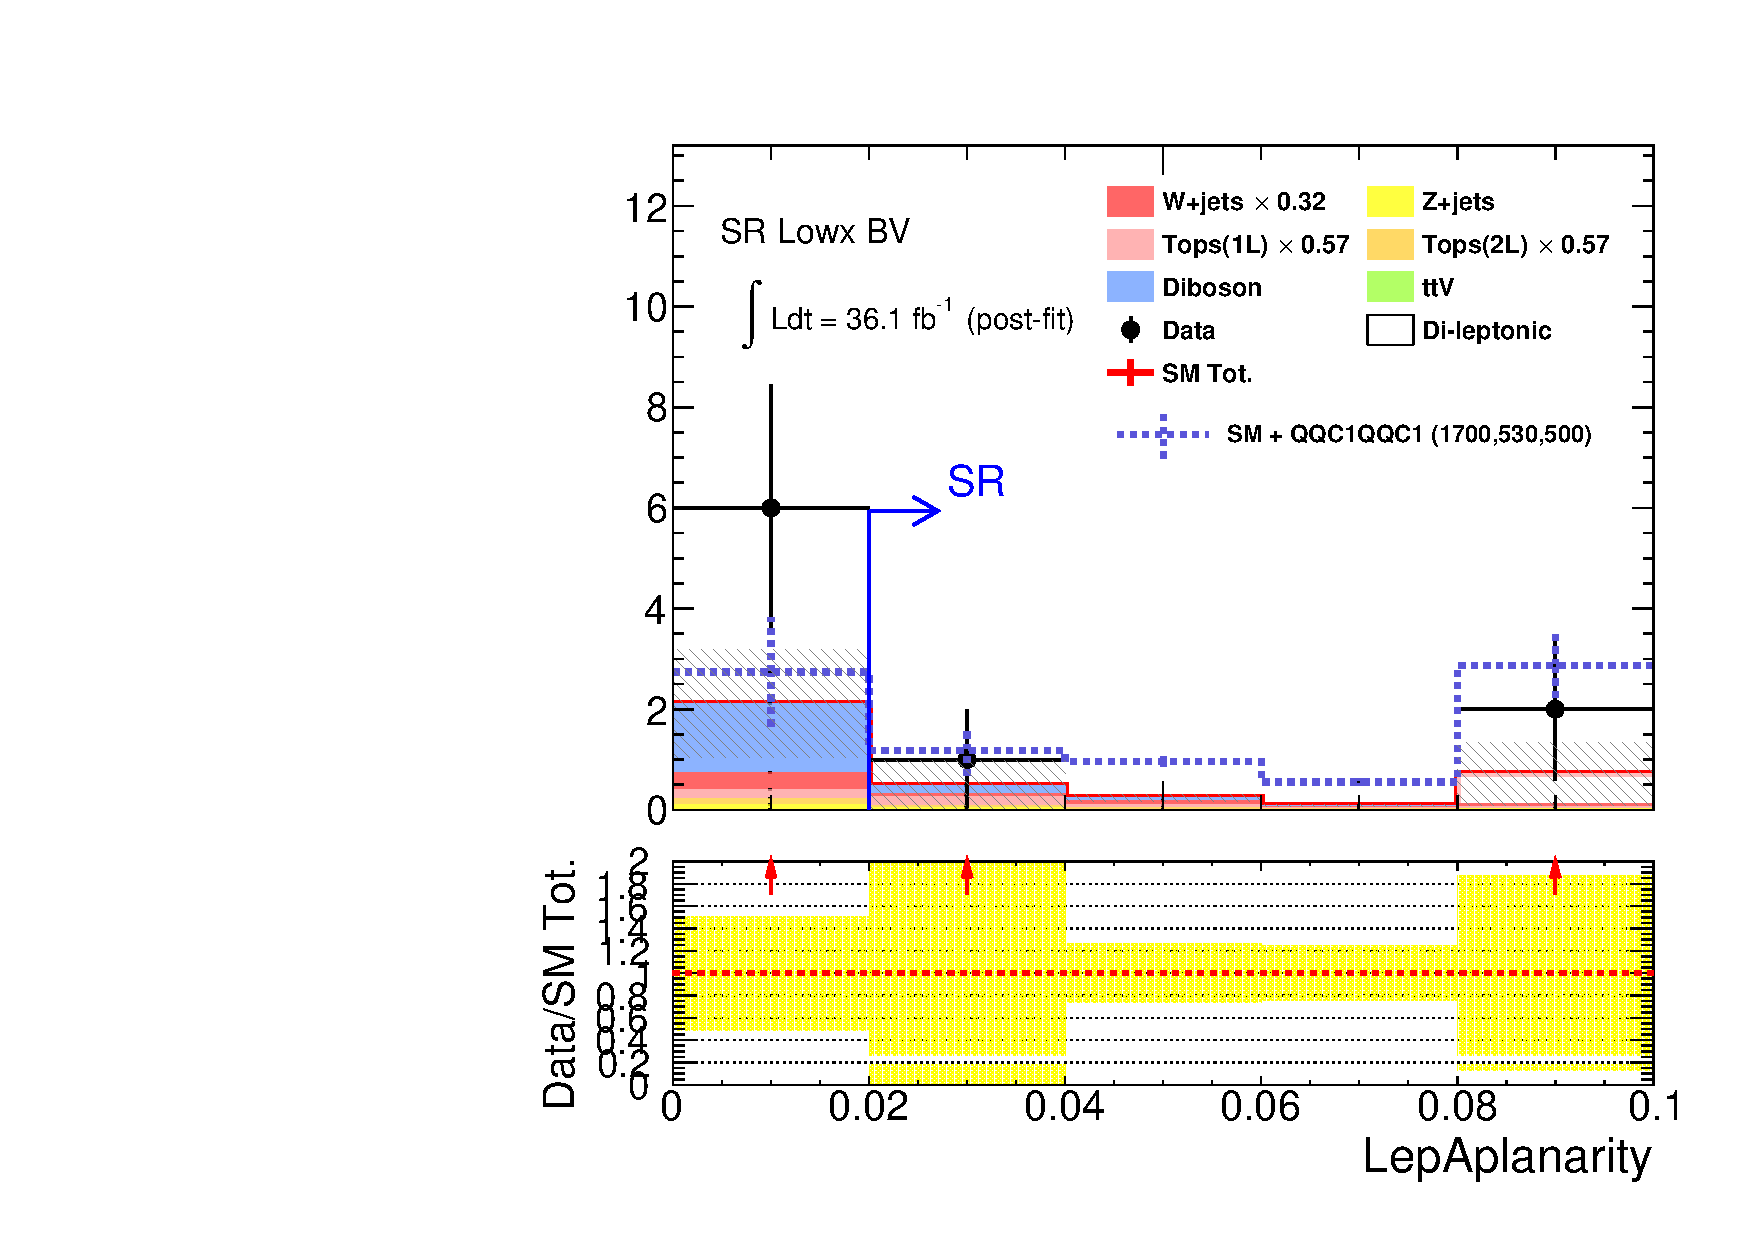
\includegraphics[width=0.41\textwidth]{figures/BGestimation/SRVRpostFit/LepAplanarity__SRLowxBV_no_LepAplanarity_postFit_2SFconfig_noYields_objRep.pdf}}
    \subfigure[]{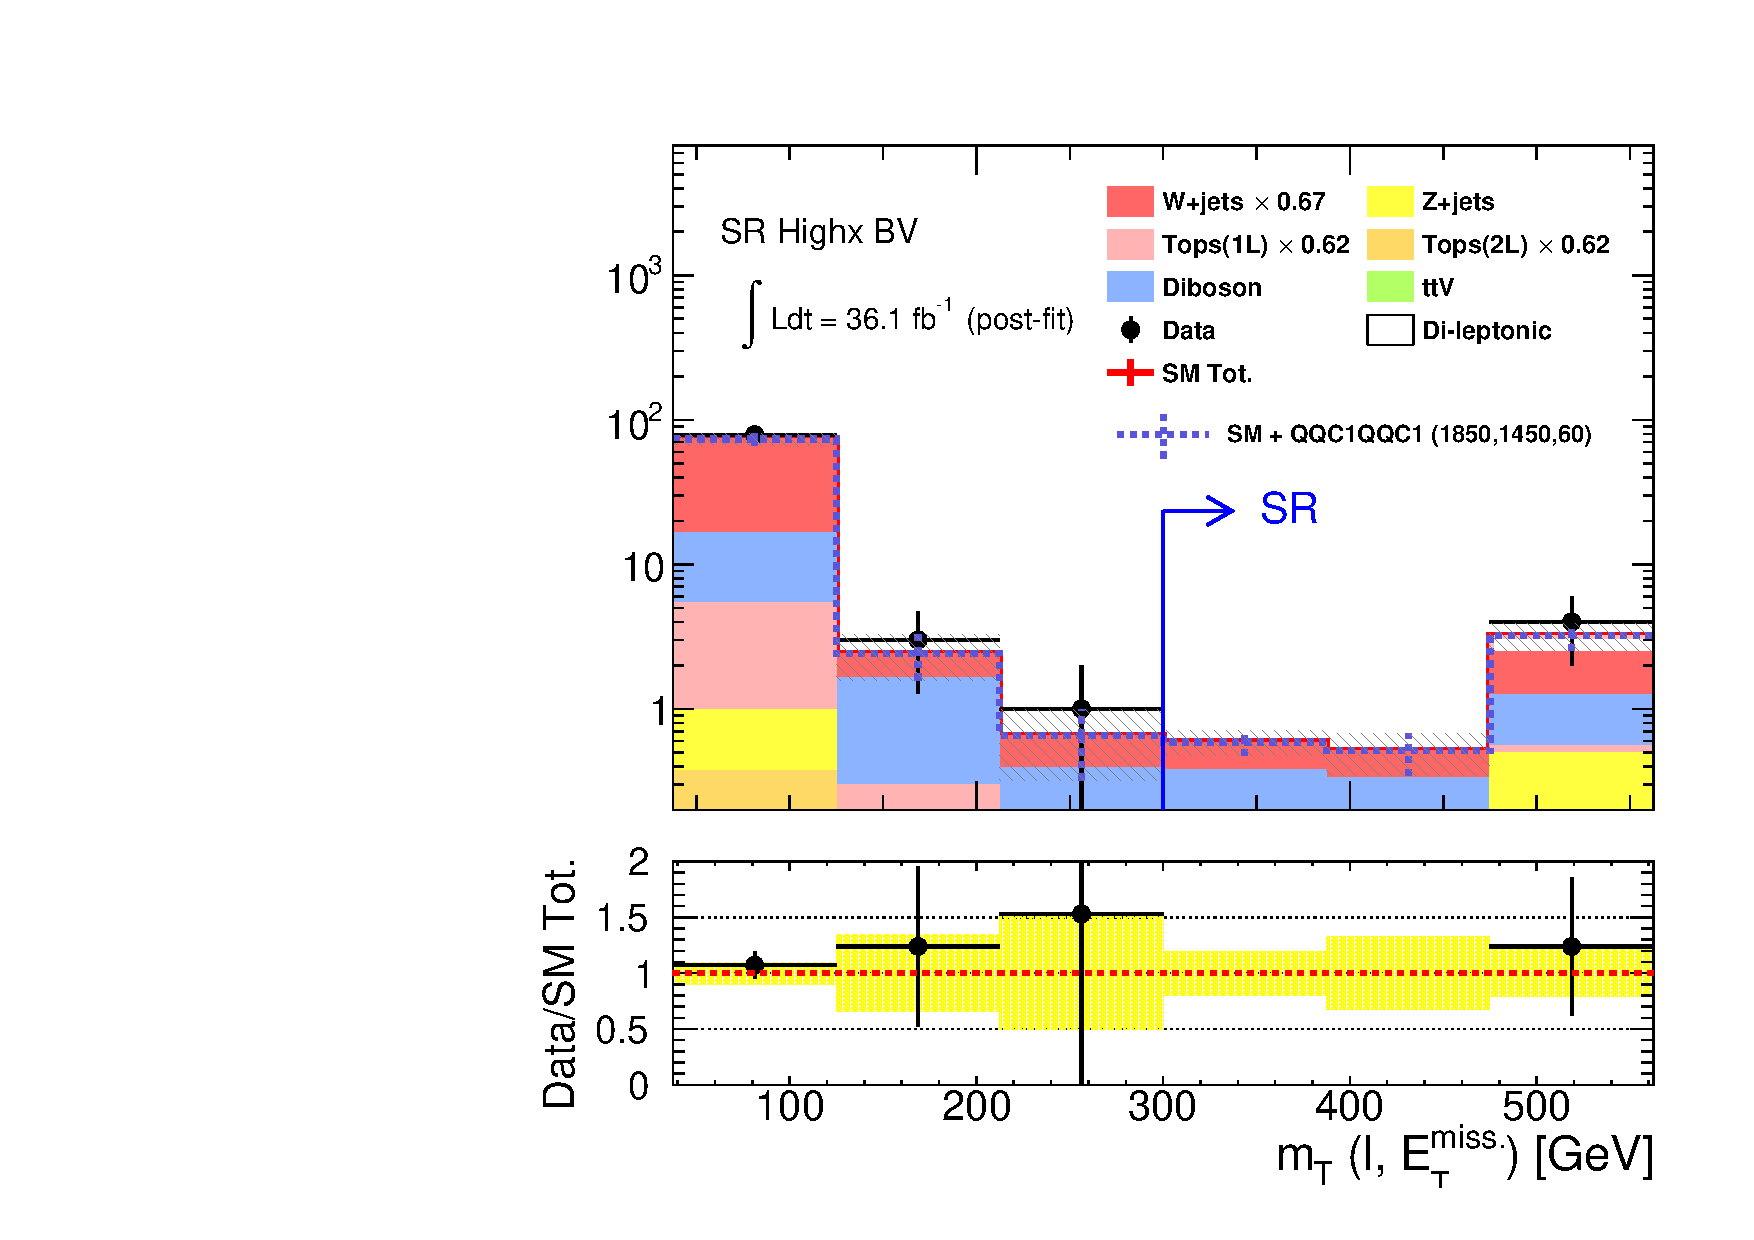
\includegraphics[width=0.41\textwidth]{figures/BGestimation/SRVRpostFit/mt__SRHighxBV_no_mt_postFit_2SFconfig_noYields_objRep.pdf}}
    \subfigure[]{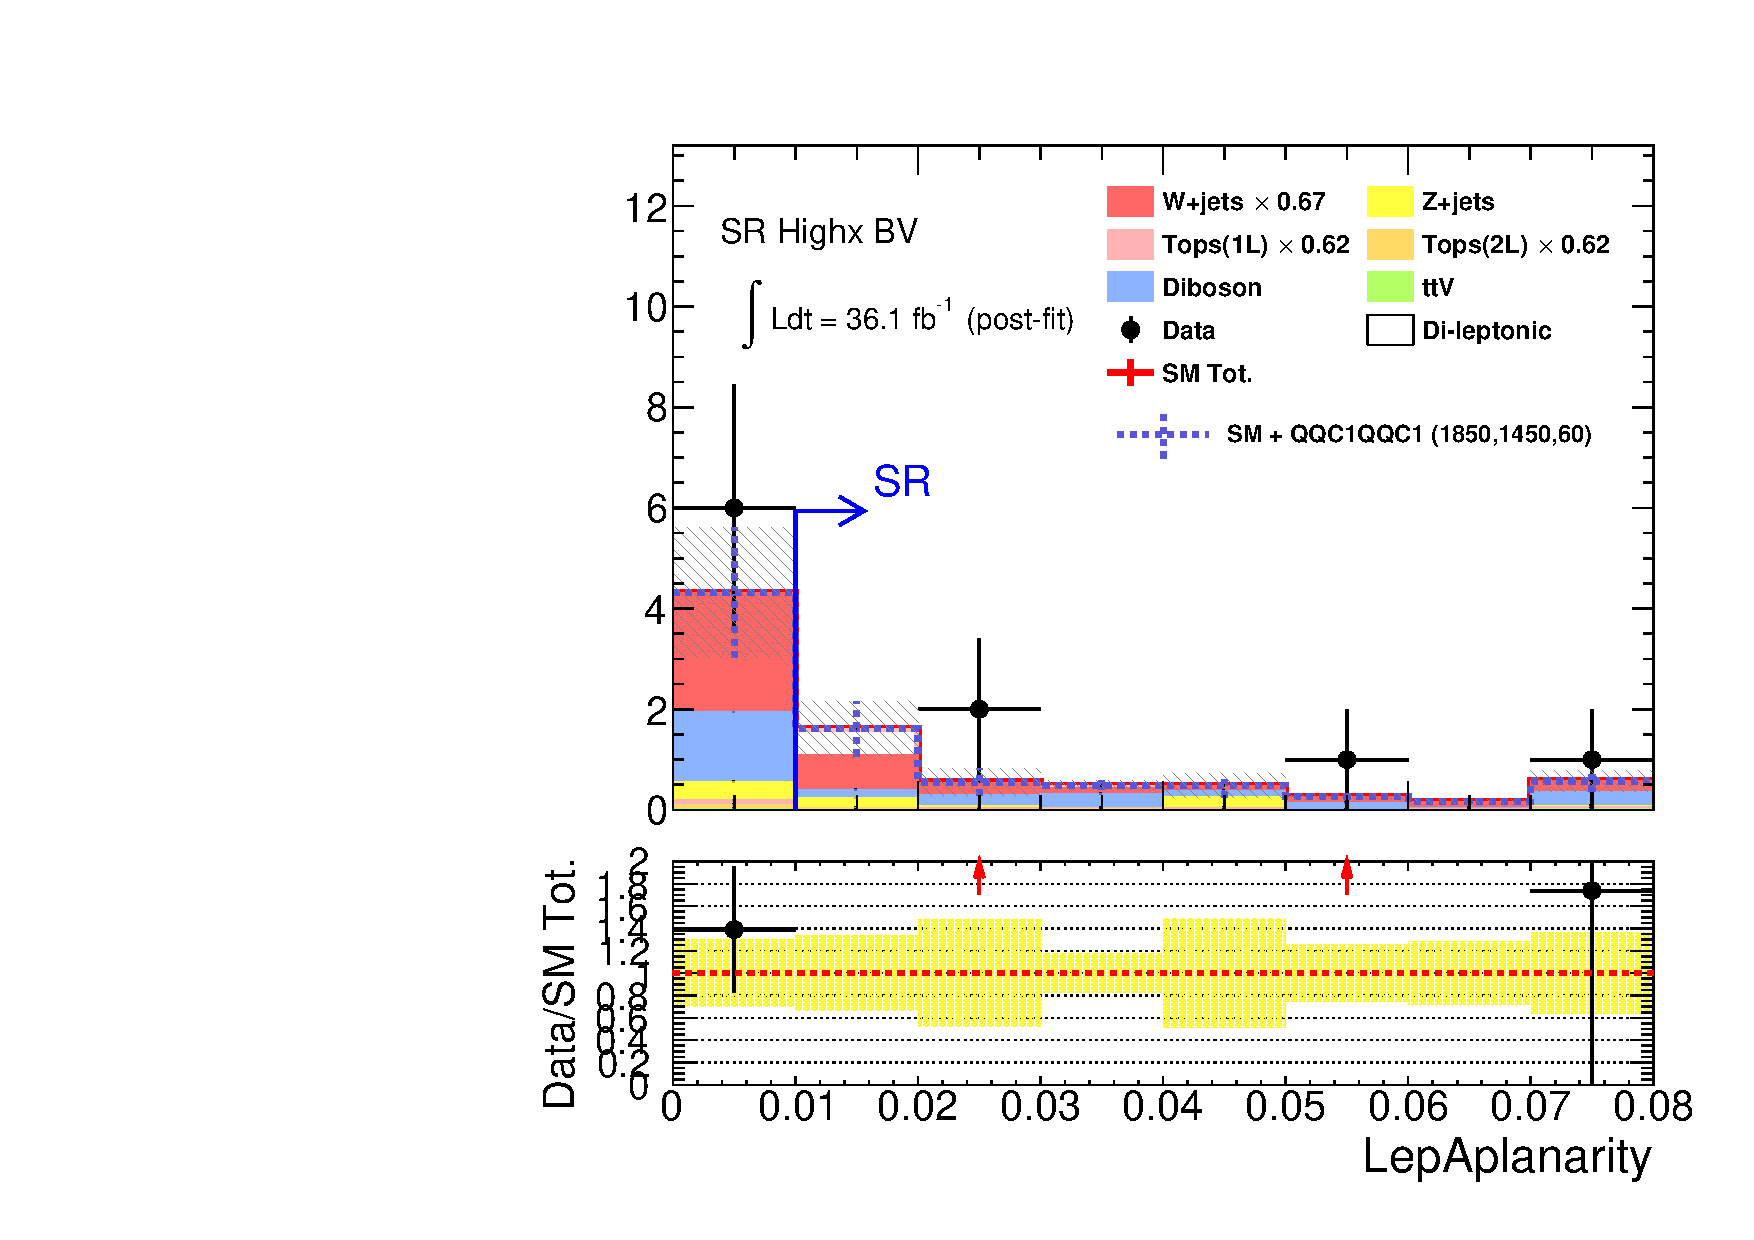
\includegraphics[width=0.41\textwidth]{figures/BGestimation/SRVRpostFit/LepAplanarity__SRHighxBV_no_LepAplanarity_postFit_2SFconfig_noYields_objRep.pdf}}
   \caption{   
     Post-fit distruibution of (left) $\mt$ and (right) $\apl$.
     (a,b) SR Low-x BV.
     (c,d) SR High-x BV.
     The yellow band in the bottom panel represents only statistical error. The overflow is included in the highest bin.  
     \label{fig::BGestimation::SRVRpostFit::SRVarxBV}
   }
\end{figure}

% ----------------------------------------------

\clearpage
% -------------- 3B ---------
\begin{figure}[h]
  \centering
    \subfigure[]{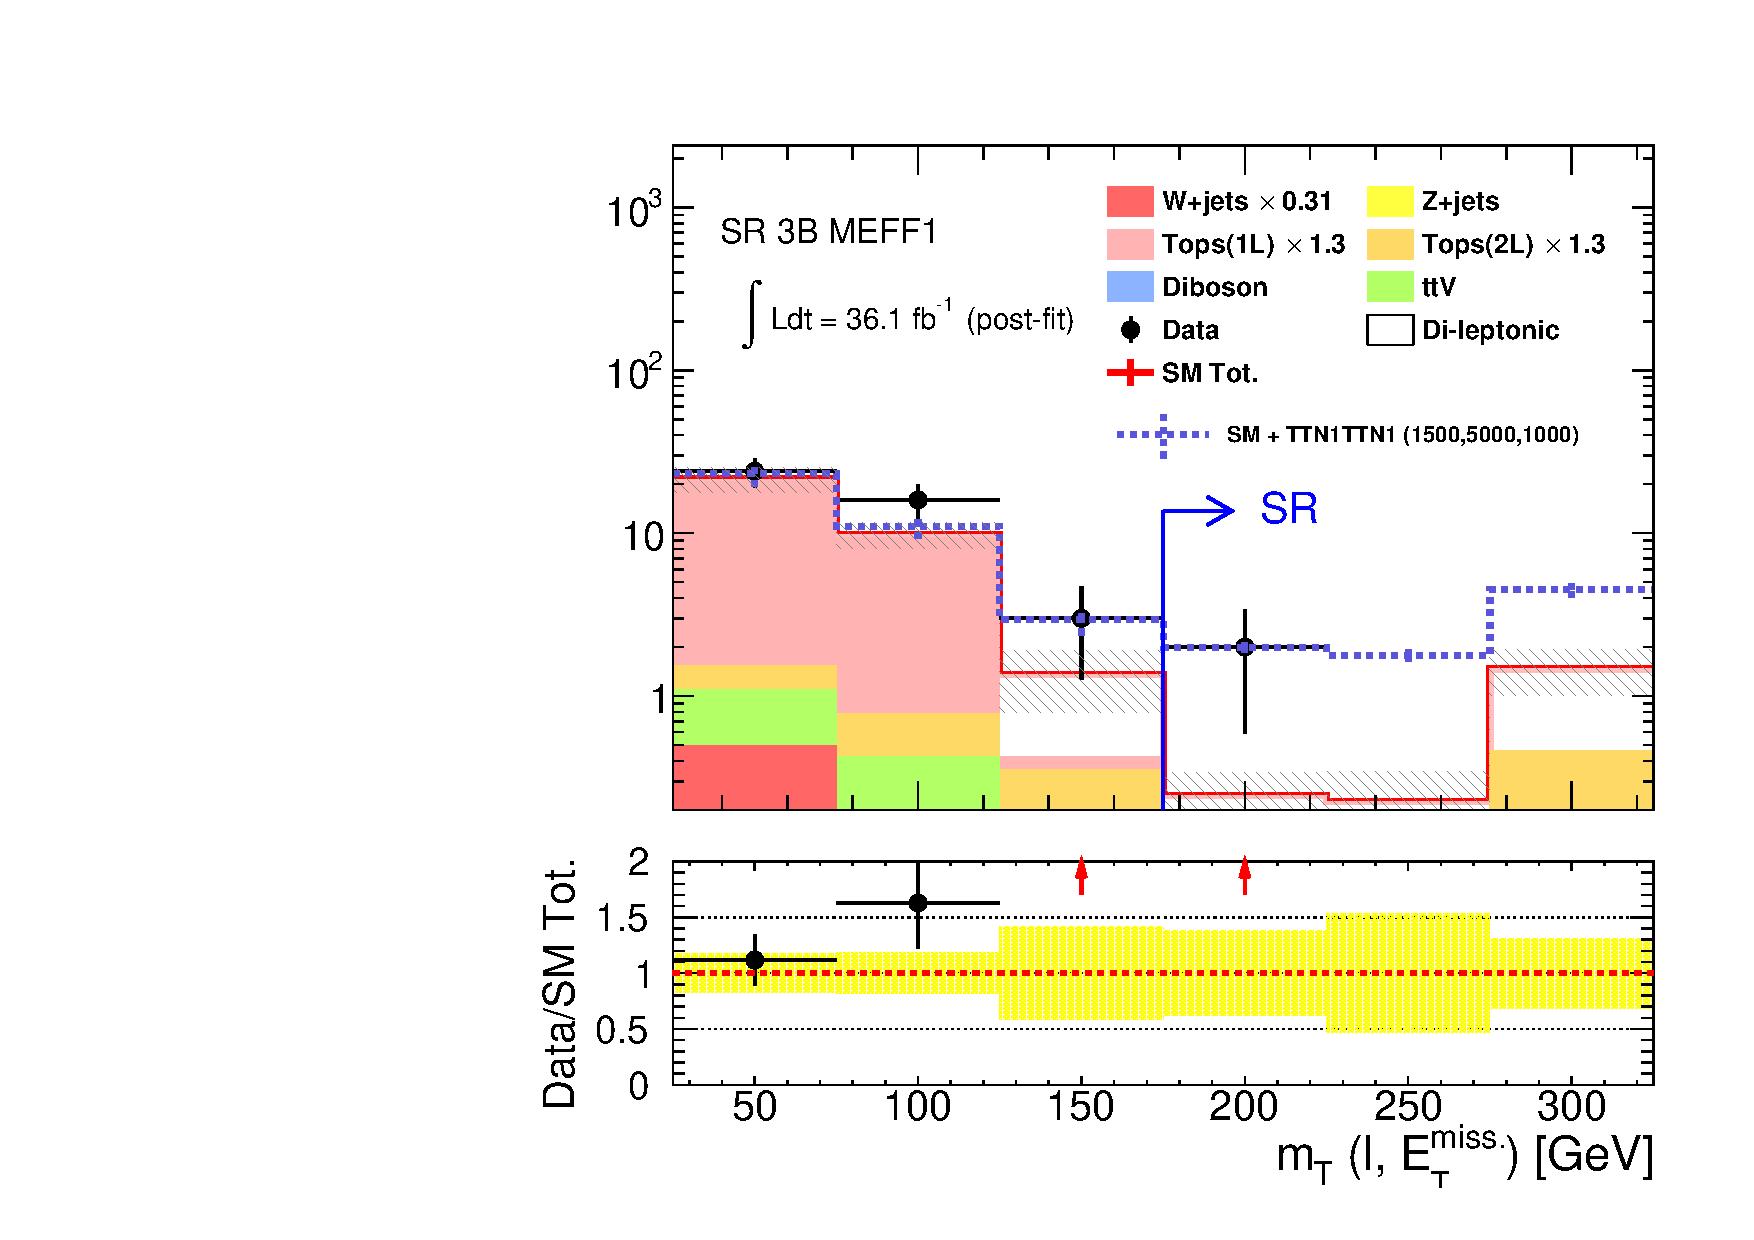
\includegraphics[width=0.41\textwidth]{figures/BGestimation/SRVRpostFit/mt__SR3BMEFF1_no_mt_postFit_2SFconfig_noYields_objRep.pdf}}
    \subfigure[]{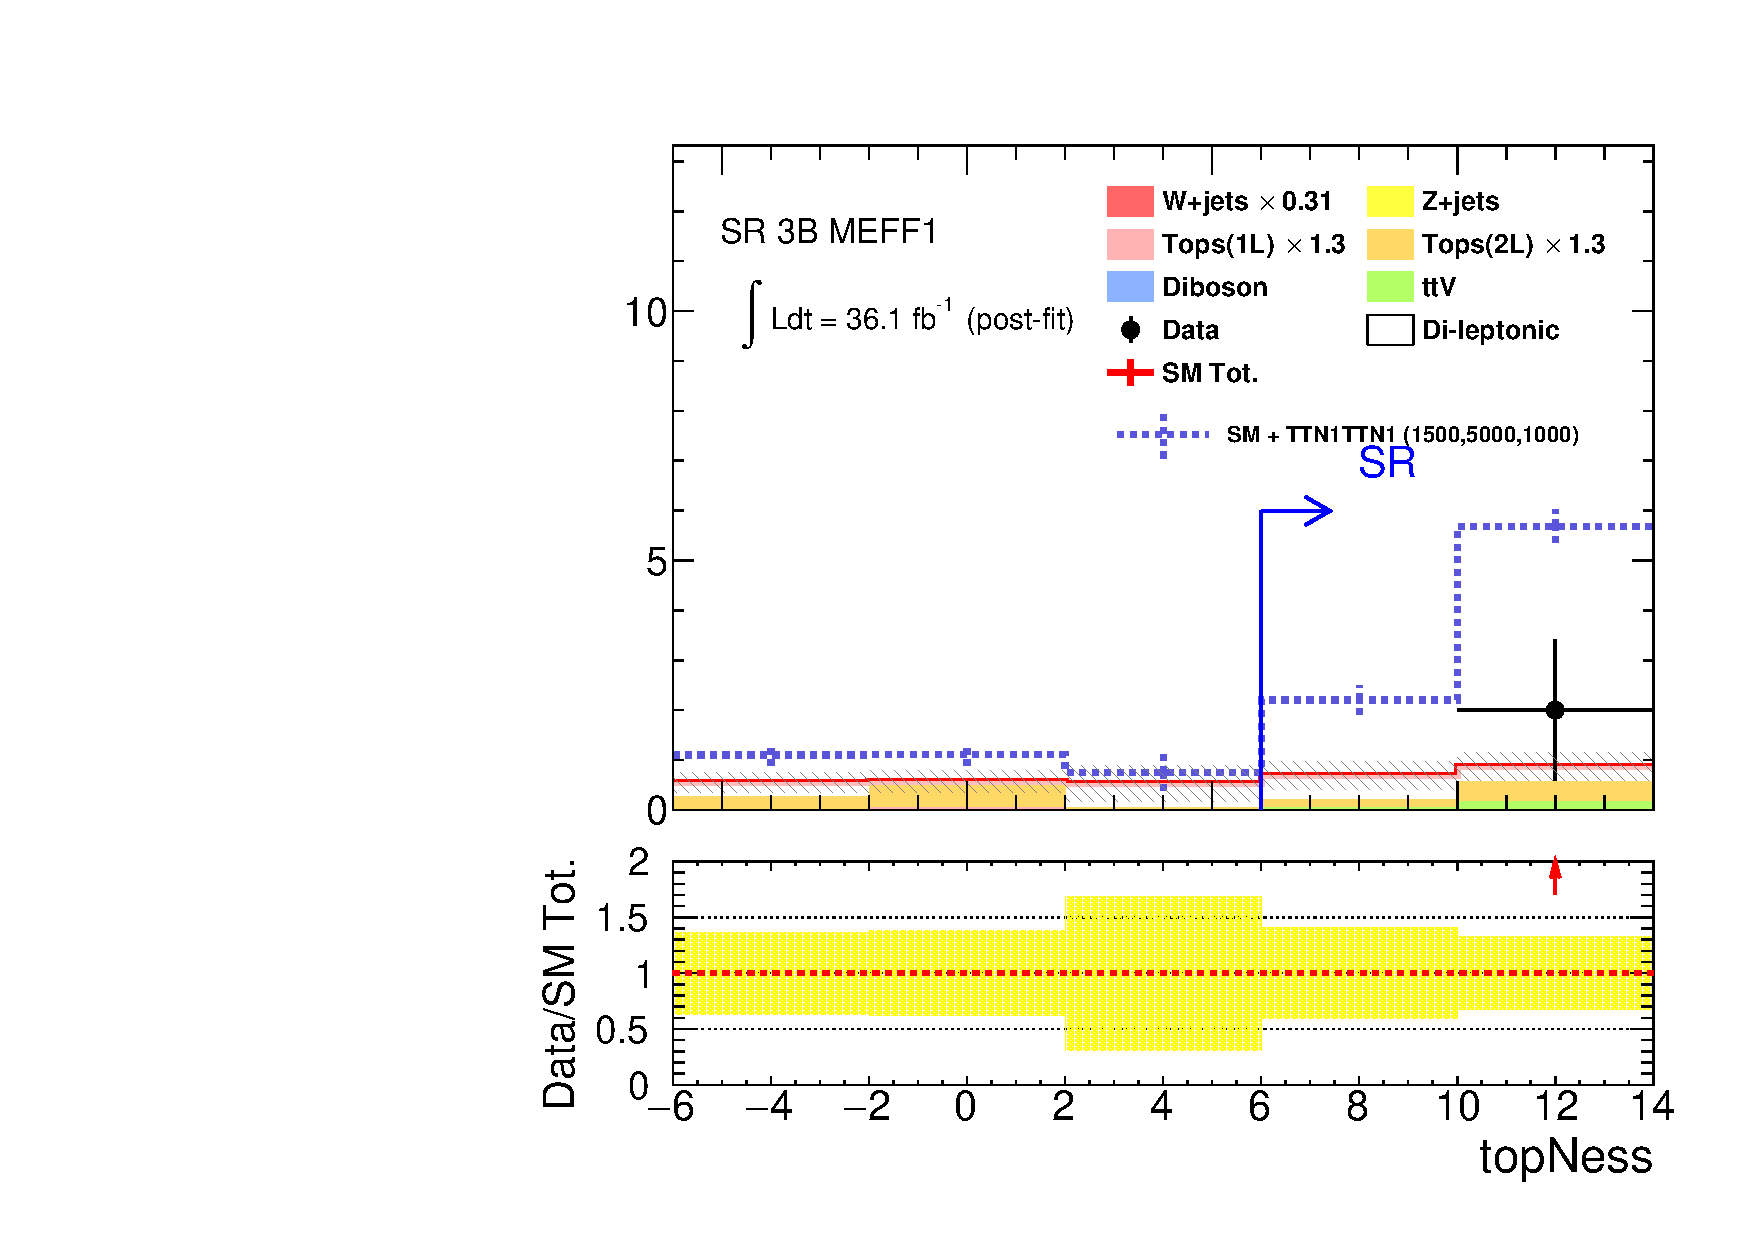
\includegraphics[width=0.41\textwidth]{figures/BGestimation/SRVRpostFit/topNess__SR3BMEFF1_no_topNess_postFit_2SFconfig_noYields_objRep.pdf}}
    \subfigure[]{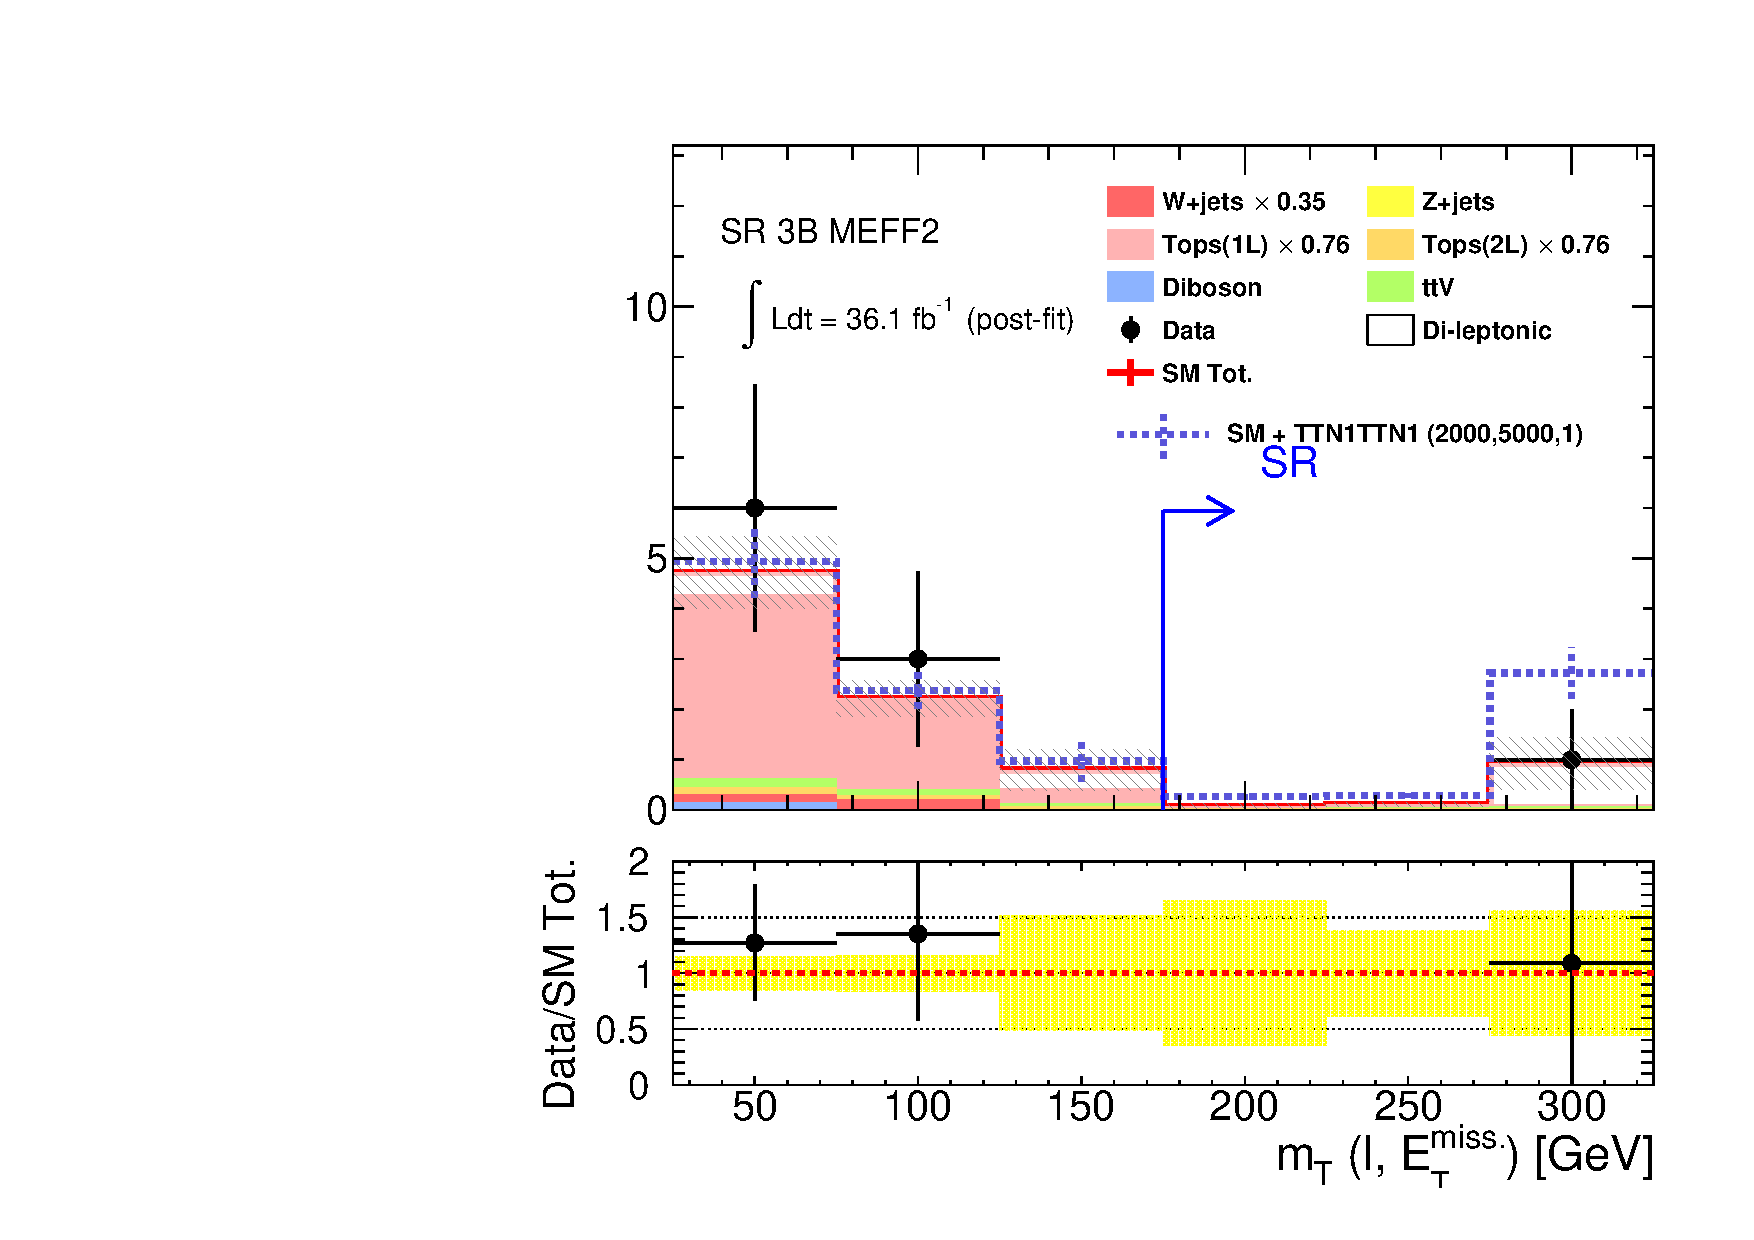
\includegraphics[width=0.41\textwidth]{figures/BGestimation/SRVRpostFit/mt__SR3BMEFF2_no_mt_postFit_2SFconfig_noYields_objRep.pdf}}
    \subfigure[]{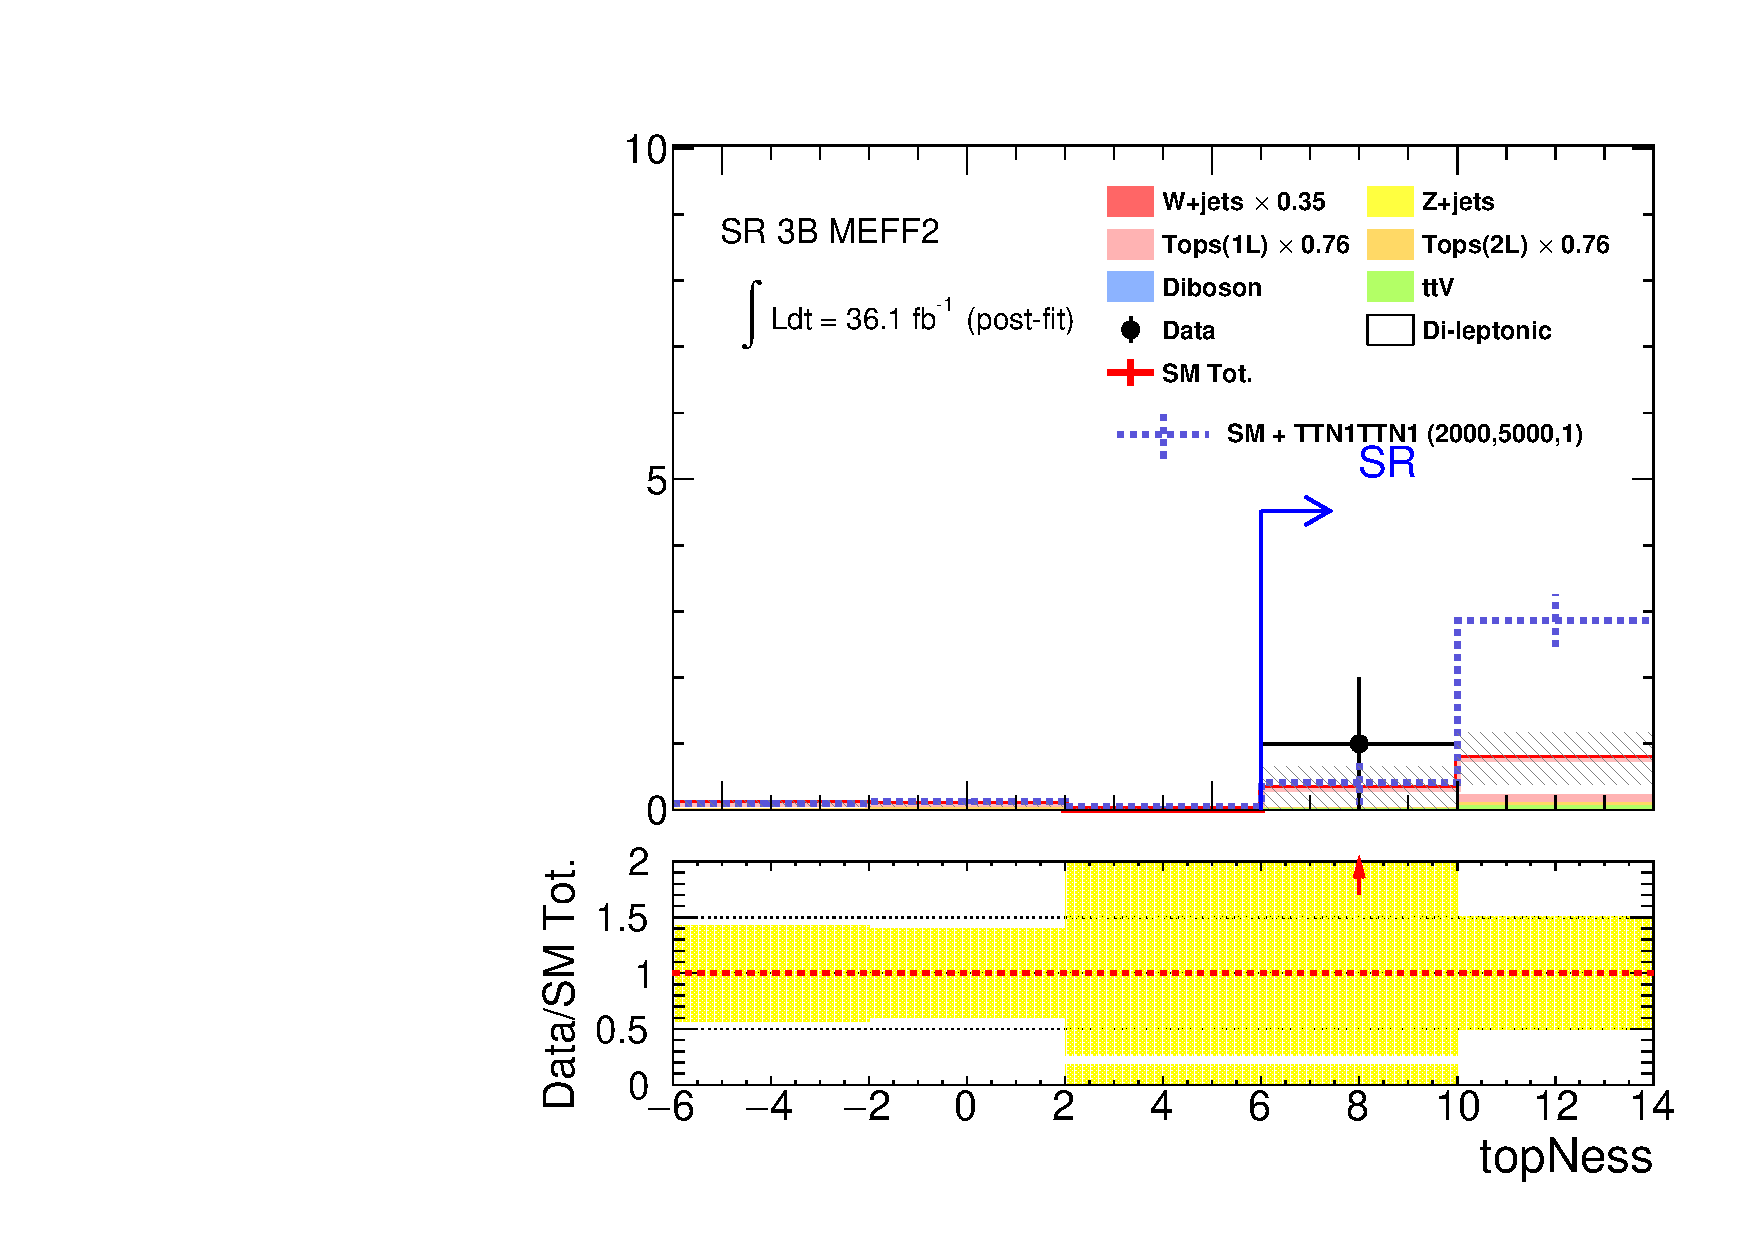
\includegraphics[width=0.41\textwidth]{figures/BGestimation/SRVRpostFit/topNess__SR3BMEFF2_no_topNess_postFit_2SFconfig_noYields_objRep.pdf}}
    \caption{   
      Post-fit distruibution of (left) $\mt$, and (right) topness.
      (a,b) SR 3B-$\meffIncFirst$.
      (c,d) SR 3B-$\meffIncSecond$.
      The yellow band in the bottom panel represents only statistical error. The overflow is included in the highest bin.  
      \label{fig::BGestimation::SRVRpostFit::SR3B}
    }
\end{figure}

